\PassOptionsToPackage{quiet}{fontspec}
\documentclass[12pt,a4paper]{article}
\usepackage{thesis} % 格式控制
\usepackage{indentfirst}
\usepackage{enumitem}
\usepackage{amsmath} % 数学公式支持
\usepackage{amsfonts} % 数学字体支持
\usepackage{amssymb} % 数学符号支持
\usepackage{graphicx} % 图片插入支持
\usepackage{float} % 浮动体位置控制，支持 [H] 选项
\usepackage{caption} % 图表标题格式控制
\usepackage{geometry} % 页面布局控制
\usepackage{setspace} % 行距控制
\usepackage{xeCJK} % 中文字体支持
\usepackage{fontspec} % 字体设置
\usepackage[most]{tcolorbox} % 高亮按键命令
\usepackage{colortbl} % 表格颜色支持
\setlength{\parindent}{2em} % 控制首行缩进  
\addtolength{\parskip}{3pt} % 控制段落距离  
\onehalfspacing % 1.5倍行距  
\graphicspath{{./figures/}} % 指定图片所在文件夹  
\setCJKmainfont{SimSun}

\classname{\heiti\bfseries 计算机组成与设计}  % 设置课程名称
\makepagestyle{}{}

\newtcbox{\keyblue}{on line,
  colframe=blue!60!black, colback=blue!10,
  boxrule=0.8pt, arc=2pt, boxsep=0pt, left=2pt, right=2pt, top=1pt, bottom=1pt,
  tcbox raise base, fontupper=\color{blue}\bfseries}

\begin{document}
\maketitlepage{Lab30 RISC-V微处理器设计}{玉泉高分子楼-201}{郑智瑄}{3230103913}{\today}{唐奕/屈民军} %封面页 

\maketoc

\section{实验目的}
\begin{enumerate}
    \item 熟悉 RISC-V 指令系统。
    \item 了解提高 CPU 性能的方法。
    \item 掌握流水线 RISC-V 微处理器的工作原理。
    \item 理解数据冒险、控制冒险的概念以及流水线冲突的解决方法。
    \item 掌握流水线 RISC-V 微处理器的测试方法。
    \item 了解用软件实现数字系统的方法。
\end{enumerate}

\section{实验任务}
\subsection{基本要求}
    设计一个流水线 RISC-V 微处理器，具体要求如下:
    \begin{enumerate}
        \item 至少运行下列 RV32I 核心指令。
        \begin{enumerate}[label=\arabic*)]
            \item 算术运算指令： add、sub、addi
            \item 逻辑运算指令： and、or、xor、slt、sltu、andi、ori、xori、slti、sltiu
            \item 移位指令： sll、srl、sra、slli、srli、srai
            \item 条件分支指令： beq、bne、blt、bge、bltu、bgeu
            \item 无条件跳转指令： jal、jalr
            \item 数据传送指令： lw、sw、lui、auipc
            \item 空指令： nop
        \end{enumerate}
        \item 采用 5 级流水线技术，对数据冒险实现转发或阻塞功能。
        \item 在 Nexys Video 开发系统中实现 RISC-V 微处理器，要求 CPU 的运行速度大于 25MHz。
    \end{enumerate}
\subsection{扩展要求}
    \begin{enumerate}
        \item 要求设计的微处理器还能运行 lb、lh、ld、lbu、lhu、lwu、sb、sh 或 sd 等字节、半字和双字数据传送指令。
        \item 要求设计的 CPU 增加异常（exception）、自陷（trap）、中断（interrupt）等处理方案。
    \end{enumerate}

\section{实验设备}
\begin{enumerate}
    \item 装有 Vivado 和 ModelSim SE 软件的计算机。
    \item Nexys Video 开发板一套。
    \item 带有 HDMI 接口的显示器一台。
\end{enumerate}

\section{提供的文件}
\begin{enumerate}
    \item 指令译码模块（decode）的测试代码 Decode\_tb.v、ALU 测试代码 ALU\_tb.v、取指令级模块（IF）的测试代码 IF\_tb.v 和 CPU 的顶层测试代码 Risc5CPU\_tb.v。
    \item 指令存储器（InstructionROM）的 Verilog HDL 代码 InstructionROM.v。
    \item 硬件测试 CPU 的 Vivado 架构。在该架构中，用带有 HDMI 接口的显示器显示 CPU 运行的内部重要变量。测试架构将程序指针的低 8 位 PC[7:0]、指令机器码 Instruction\_id、流水线气泡插入标志 Stall、跳转标记 JumpFlag、ALU 操作数 A 及 B、ALU 结果 ALUResult 和数据存储输出 MemDout\_mem 等送入带有 HDMI 接口的显示器，显示格式如图 Figure1 所示。
    
    \begin{figure}[H]
        \centering
        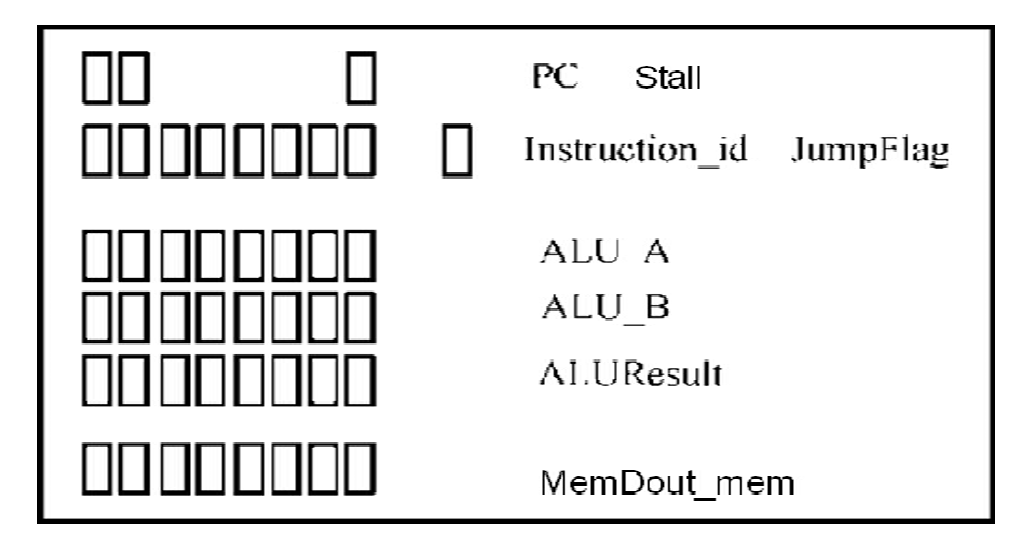
\includegraphics[width=0.6\textwidth]{e1.png}
        \caption{VGA 显示格式}

    \end{figure}
    
    当完成整个流水线 CPU 的设计与仿真测试，打开 Vivado 文件夹下的 Risc5CPU.xpr 工程，添加流水线 CPU 设计代码（包括子模块代码），然后综合、实现和下载至开发板，连接带有 HDMI 接口的显示器就可进行测试。
\end{enumerate}

\clearpage
\section{实验内容}
\begin{enumerate}
    \item 从网络下载相关文件。
    \item 编写指令译码单元 Decode 模块的 Verilog HDL 代码，并用 ModelSim 进行功能仿真。
    \item 编写寄存器堆 Register 模块的 Verilog HDL 代码。
    \item 编写 ID 模块 Verilog HDL 代码，ID.v 文件已给端口列表。
    \item 编写 ALU 模块的 Verilog HDL 代码并用 ModelSim 进行功能仿真。
    \item 编写执行单元 EX 模块的 Verilog HDL 代码，EX.v 文件已给端口列表。
    \item 编写 IF 模块的 Verilog HDL 代码并用 ModelSim 进行功能仿真。
    \item 打开 Vivado 文件夹下的 Risc5CPU.xpr 工程，生成符合 CPU 要求的数据存储器 IP 内核。
    \item 编写 CPU 顶层的 Verilog HDL 代码，并用 ModelSim 进行功能仿真。注意：由于存在 IP 内核，仿真时，需加仿真库，方法参考实验 3。
    \item 再次打开 Vivado 文件夹下的 Risc5CPU.xpr 工程；添加流水线 CPU 设计的全部代码，然后综合、实现和下载至 Nexys Video 开发板。
    \item 连接带有 HDMI 接口的显示器，进行测试。首先将 SW0 置于低电平，使 RISC-V CPU 工作在“单步”运行模式。复位后，每按一下上边按键，RISC-V CPU 运行一步，记录下显示器上的结果，对照Figure2验证设计是否正确。
\end{enumerate}

\begin{figure}[H]
    \centering
    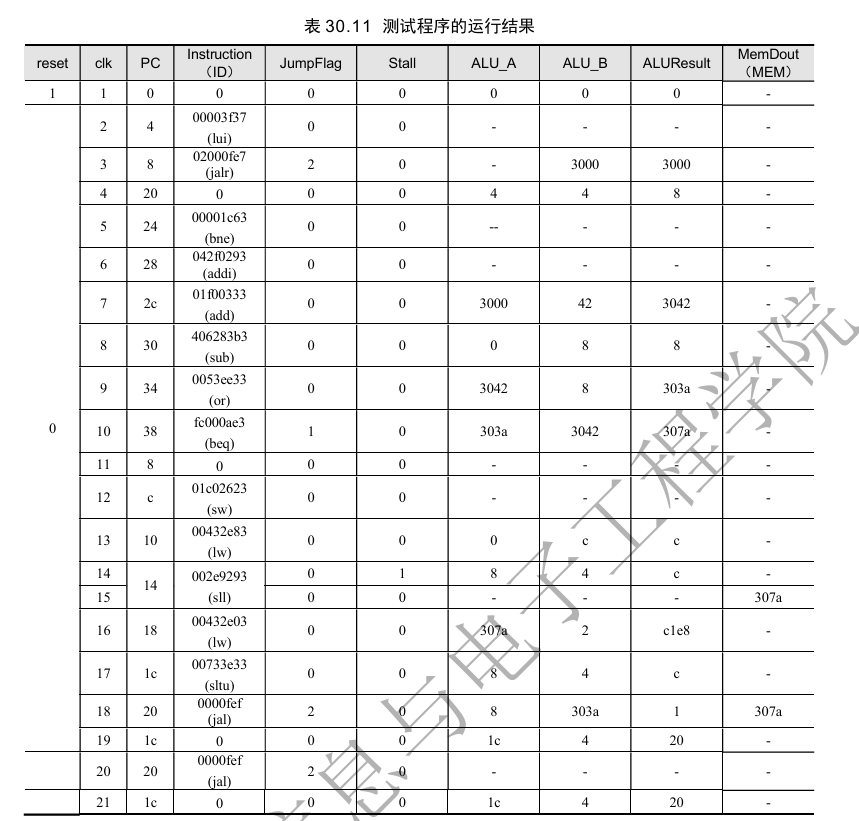
\includegraphics[width=1\textwidth]{e2.png}
    \caption{测试程序运行结果}
\end{figure}
\clearpage
\section{实验过程}
\subsection{Decode模块设计}
\subsubsection{设计原理}

该子模块主要作用是根据指令确定各个控制信号的值，同时产生立即数 Imm 和偏移量 offset。该模块是一个组合电路。

RISC-V 将指令分为 R、I、S、SB、U、UJ 等六类。仔细分析表 30.2 指令表，从电路设计角度看，根据操作数的来源和立即数构成方式不同，再次细分指令。具体做法：

\begin{itemize}
    \item R\_type 类：操作码（opcode，简称 op）为 7'h33，R 类的所有指令，两个操作数分别为 rs1 和 rs2；
    \item I\_type 类：操作码 7'h13，I 类的算术逻辑运算指令和移位指令，两个操作数分别为 rs1 和立即数 imm；
    \item LW 指令：操作码 7'h03，I 类的数据传送指令 lw，两个操作数分别为 rs1 和立即数 imm；
    \item JALR 指令：操作码 7'h67，I 类的无条件分支指令 jalr，两个操作数分别为 PC 和常数 4；
    \item SW 指令：操作码 7'h23，S 类的数据传送指令 sw，两个操作数分别为 rs1 和立即数 imm；
    \item SB\_type 类：操作码 7'h63，SB 类的所有指令，两个操作数分别为 PC 和立即数 imm；
    \item LUI 指令：操作码 7'h37，U 类的数据传送指令 lui，只有一个操作数（立即数 imm）；
    \item AUIPC 指令：操作码 7'h17，U 类的数据传送指令 auipc，两个操作数分别为 PC 和立即数 imm；
    \item JAL 指令：操作码 7'h6F，UJ 类的无条件分支指令 jal，两个操作数分别为 PC 和常数 4。
\end{itemize}

因此，设置 R\_type、I\_type、SB\_type、LW、JALR、SW、LUI、AUIPC 和 JAL 等变量来表示指令类型，各变量的值由式(6.1.1)决定。

\begin{equation}
\begin{cases}
\text{R\_type} = (\text{op} == \text{R\_type\_op}) \\
\text{I\_type} = (\text{op} == \text{I\_type\_op}) \\
\text{SB\_type} = (\text{op} == \text{SB\_type\_op}) \\
\text{LW} = (\text{op} == \text{LW\_op}) \\
\text{JALR} = (\text{op} == \text{JALR\_op}) \\
\text{SW} = (\text{op} == \text{SW\_op}) \\
\text{LUI} = (\text{op} == \text{LUI\_op}) \\
\text{AUIPC} = (\text{op} == \text{AUIPC\_op}) \\
\text{JAL} = (\text{op} == \text{JAL\_op})
\end{cases}
\tag{6.1.1}
\end{equation}

(1)只有 LW 指令读取存储器且回写数据取自存储器，所以有

\begin{equation}
\text{MemtoReg}=\text{LW}
\tag{6.1.2}
\end{equation}

\begin{equation}
\text{MemRead}=\text{LW}
\tag{6.1.3}
\end{equation}

(2)只有 SW 指令会对存储器写数据，所以有

\begin{equation}
\text{MemWrite}=\text{SW}
\tag{6.1.4}
\end{equation}

(3)需要进行回写的指令类型有 R\_type、I\_type、LW、JALR、LUI、AUIPC 和 JAL。所以有

\begin{equation}
\text{RegWrite}=\text{R\_type} \parallel \text{I\_type} \parallel \text{LW} \parallel \text{JALR} \parallel \text{LUI} \parallel \text{AUIPC} \parallel \text{JAL}
\tag{6.1.5}
\end{equation}

(4)只有 JALR 和 JAL 两条无条件分支指令，所以有

\begin{equation}
\text{Jump}=\text{JALR} \parallel \text{JAL}
\tag{6.1.6}
\end{equation}

(5)操作数 A 和 B 的选择信号的确定

分析各类指令，可得到Figure 3操作数选择的功能表。

\begin{figure}[H]
    \centering
    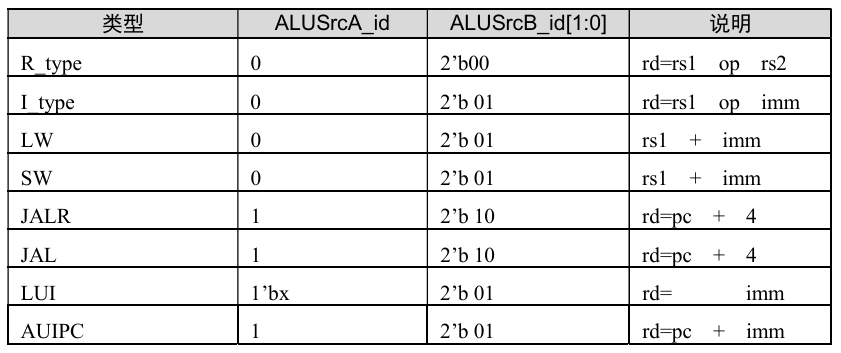
\includegraphics[width=0.8\textwidth]{e3.png}
    \caption{操作数选择信号的功能表}
\end{figure}

从Figure 3可获得 ALUSrcA\_id 和 ALUSrcB\_id[1:0]表达式。

\begin{equation}
\text{ALUSrcA} = \text{JALR} \parallel \text{JAL} \parallel \text{AUIPC}
\tag{6.1.7}
\end{equation}

\begin{align}
\text{ALUSrcB}[1] &= \text{JAL} \parallel \text{JALR} \tag{6.1.8a} \\
\text{ALUSrcB}[0] &= \sim (\text{R\_type} \parallel \text{JAL} \parallel \text{JALR}) \tag{6.1.8b}
\end{align}

(6)ALUCode 的确定

除了条件分支指令，其它指令都需要 ALU 执行运算，共有 11 种不同运算，ALUCode 信号需用 4 位二进制表示。最主要为加法运算，设为默认算法，ALUCode 的功能表如Figure 4所示。注意：表中 funct7[6] 与 funct6[5] 在指令中为同一位置，即 instruction[30]。

\begin{figure}[H]
    \centering
    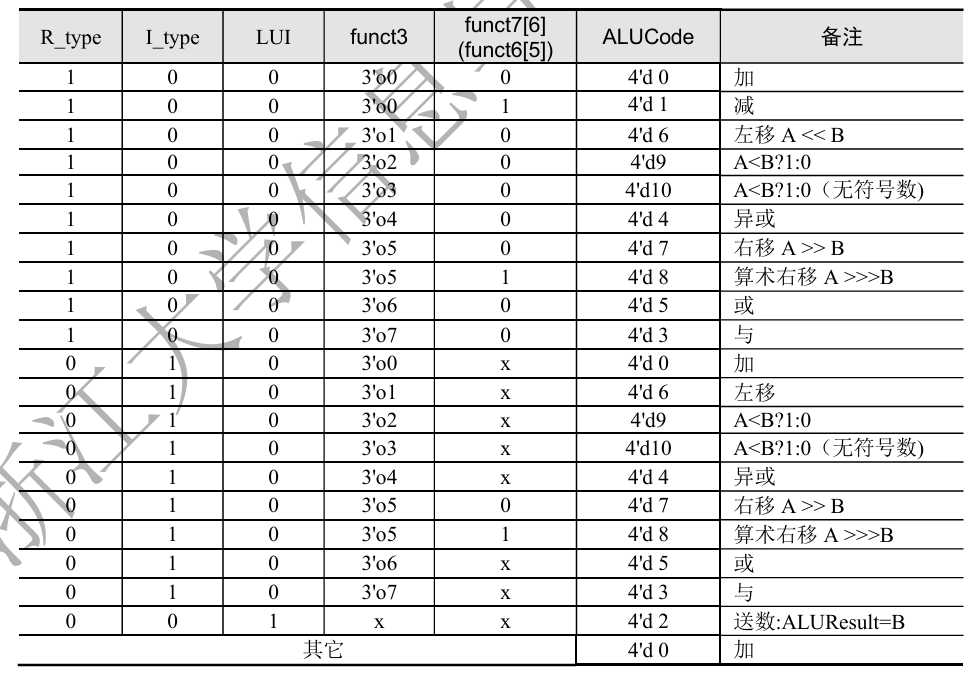
\includegraphics[width=0.9\textwidth]{e4.png}
    \caption{ALUCode 的功能表}
\end{figure}

(7)立即数产生电路（ImmGen）设计

I\_type、SB\_type、LW、JALR、SW、LUI、AUIPC 和 JAL 这几类指令均用到立即数。由于 I\_type 的算术逻辑运算与移位运算指令的立即数构成方法不同，这里再设定一个变量 Shift 来区分两者。Shift=1 表示移位运算，否为则算术逻辑运算。Shift 值由式(6.1.9)计算。

\begin{equation}
\text{Shift}= (\text{funct3}==1) \parallel (\text{funct3}==5)
\tag{6.1.9}
\end{equation}

立即数构成和扩展方法如Figure 5，Figure 6所示，表中的 inst 即 instruction。

\begin{figure}[H]
    \centering
    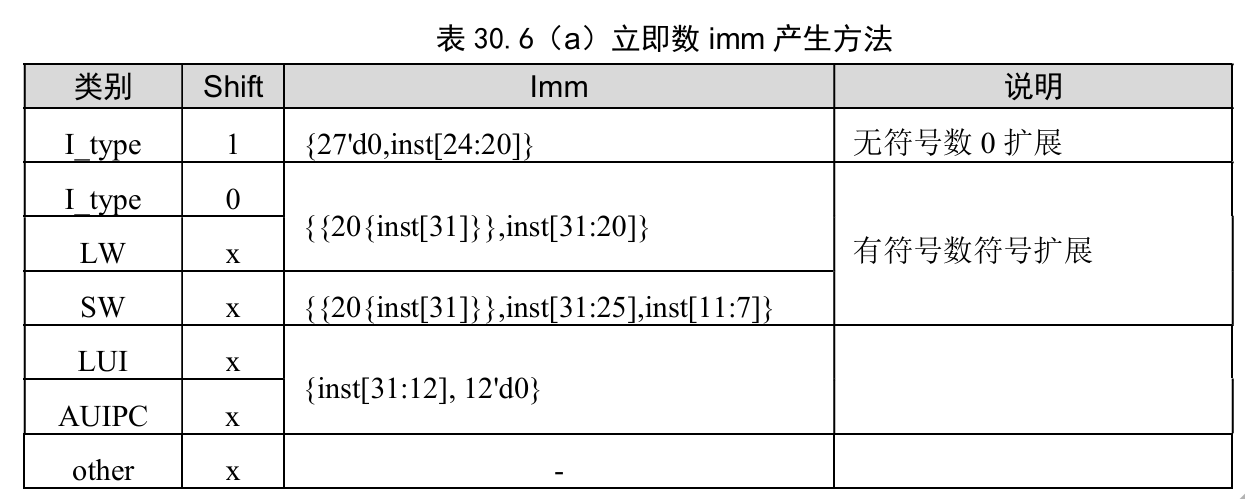
\includegraphics[width=0.8\textwidth]{e5a.png}
    \caption{立即数 imm 产生方法}
\end{figure}

\begin{figure}[H]
    \centering
    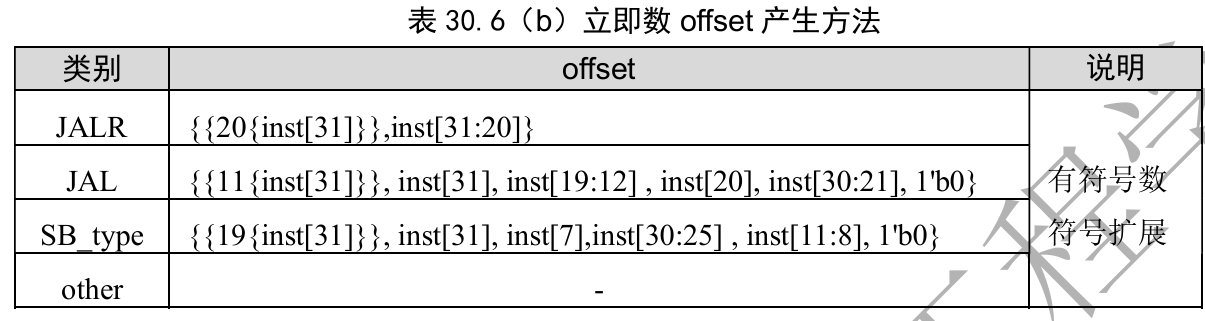
\includegraphics[width=0.8\textwidth]{e5b.png}
    \caption{立即数 offset 产生方法}
\end{figure}

\subsubsection{Verilog HDL代码与设计分析}

\textbf{(1) 指令类型识别}

根据操作码（opcode）定义各类指令类型信号，用于后续控制逻辑的判断。

\begin{lstlisting}[language=verilog]
//Define instruction types	
	wire R_type = (op == R_type_op);
	wire I_type = (op == I_type_op);
	wire SB_type = (op == SB_type_op);
	wire LW = (op == LW_op);
	wire JALR_w = (op == JALR_op);
	wire SW = (op == SW_op);
	wire LUI = (op == LUI_op);
	wire AUIPC = (op == AUIPC_op);
	wire JAL_w = (op == JAL_op);
\end{lstlisting}

\textbf{(2) 存储器控制信号生成}

根据指令类型生成存储器读写控制信号和回写数据源选择信号。只有 LW 指令需要读存储器并将存储器数据写回寄存器，只有 SW 指令需要写存储器。

\begin{lstlisting}[language=verilog]
//Control signals for memory operations
	assign MemtoReg = LW;
	assign MemRead = LW;
	assign MemWrite = SW;
\end{lstlisting}

\textbf{(3) 寄存器写控制信号生成}

需要写回寄存器堆的指令包括：R\_type、I\_type、LW、JALR、LUI、AUIPC 和 JAL。使用逻辑或运算组合这些信号。

\begin{lstlisting}[language=verilog]
//Control signal for register write
	assign RegWrite = R_type | I_type | LW | JALR_w | LUI | AUIPC | JAL_w;
\end{lstlisting}

\textbf{(4) 跳转控制信号生成}

JALR 和 JAL 为无条件跳转指令，生成相应的跳转控制信号。

\begin{lstlisting}[language=verilog]
//Jump and JALR control signals
	assign JALR = JALR_w;
	assign Jump = JAL_w;
\end{lstlisting}

\textbf{(5) ALU 操作数选择信号生成}

根据指令类型确定 ALU 的两个操作数来源。ALUSrcA 控制操作数 A 的选择（PC 或 rs1），ALUSrcB 控制操作数 B 的选择（rs2、立即数或常数 4）。

\begin{lstlisting}[language=verilog]
//ALU source A selection
	assign ALUSrcA = JALR_w | JAL_w | AUIPC;

//ALU source B selection
	assign ALUSrcB[1] = JALR_w | JAL_w;
	assign ALUSrcB[0] = ~(R_type | JALR_w | JAL_w);
\end{lstlisting}

\textbf{(6) ALU 操作码生成}

根据指令类型和功能码（funct3、funct7）确定 ALU 执行的具体运算。采用嵌套条件运算符实现多路选择，涵盖加减、逻辑运算、移位和比较等 11 种运算。

\begin{lstlisting}[language=verilog]
//ALU operation code
	assign ALUCode = LUI ? alu_lui :
	                 (R_type | I_type) ?
	                   ( (funct3 == 3'b000) ? (R_type & funct6_7 ? alu_sub : alu_add) :
	                     (funct3 == 3'b001) ? alu_sll :
	                     (funct3 == 3'b010) ? alu_slt :
	                     (funct3 == 3'b011) ? alu_sltu :
	                     (funct3 == 3'b100) ? alu_xor :
	                     (funct3 == 3'b101) ? (funct6_7 ? alu_sra : alu_srl) :
	                     (funct3 == 3'b110) ? alu_or :
	                     (funct3 == 3'b111) ? alu_and :
	                     alu_add
	                   ) :
	                 alu_add;
\end{lstlisting}

\textbf{(7) 立即数和偏移量生成}

根据不同指令类型，从指令的不同位域提取并扩展立即数（Imm）和偏移量（offset）。移位指令的立即数仅取低 5 位，其他指令需进行符号扩展。

\begin{lstlisting}[language=verilog]
//Generate immediate and offset values
	wire Shift = I_type & ((funct3 == 3'b001) | (funct3 == 3'b101));

	assign Imm = Shift ? {27'd0, Instruction[24:20]} :
	             (I_type | LW) ? {{20{Instruction[31]}}, Instruction[31:20]} :
	             SW ? {{20{Instruction[31]}}, Instruction[31:25], Instruction[11:7]} :
	             (LUI | AUIPC) ? {Instruction[31:12], 12'b0} :
	             32'd0;

	assign offset = JALR_w ? {{20{Instruction[31]}}, Instruction[31:20]} :
	                JAL_w ? {{11{Instruction[31]}}, Instruction[31], Instruction[19:12], Instruction[20], Instruction[30:21], 1'b0} :
	                SB_type ? {{19{Instruction[31]}}, Instruction[31], Instruction[7], Instruction[30:25], Instruction[11:8], 1'b0} :
	                32'd0;
\end{lstlisting}

\subsubsection{ModelSim仿真波形}

\begin{figure}[H]
    \centering
    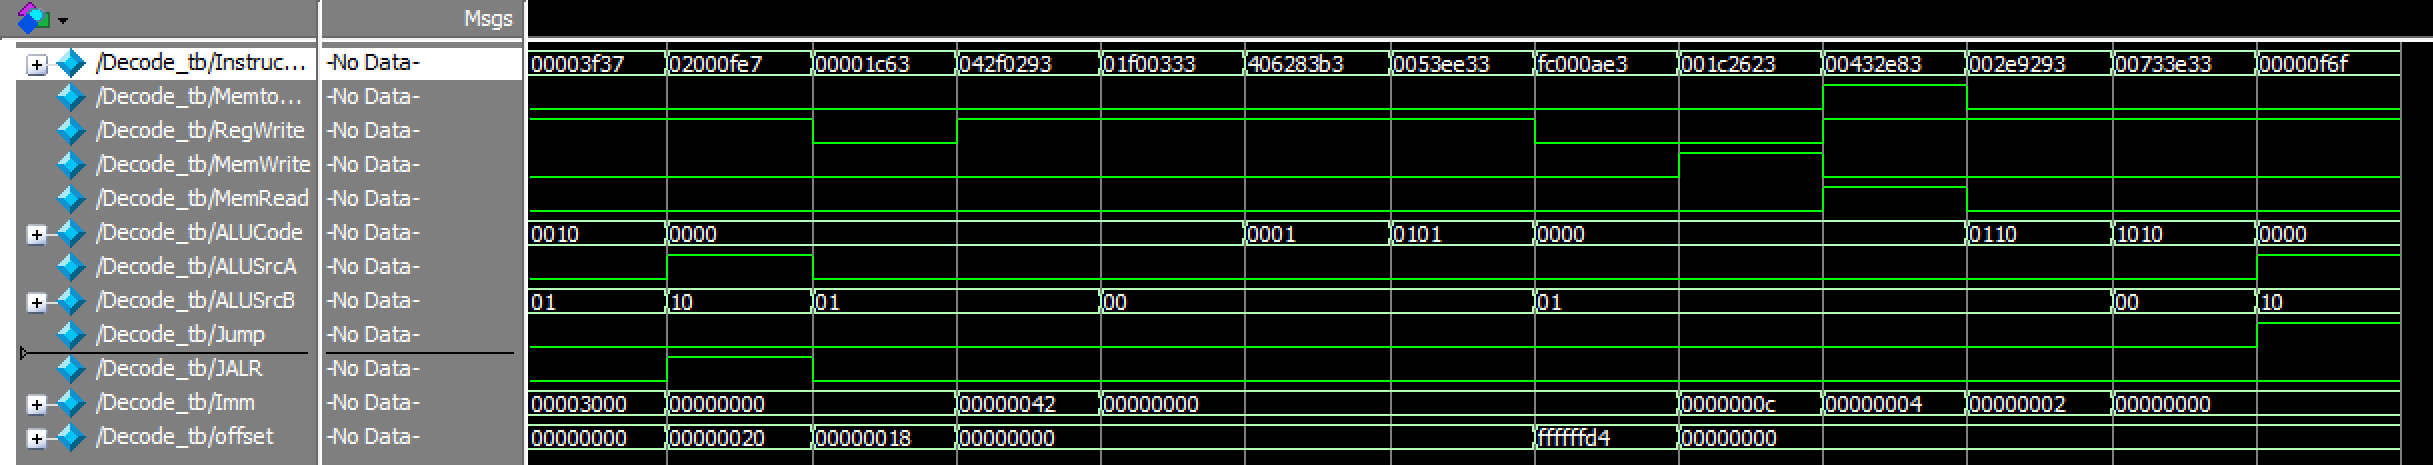
\includegraphics[width=1\textwidth]{p1.png}
    \caption{Decode模块仿真波形}
\end{figure}

\subsubsection{实验结果分析}

通过 ModelSim 对 Decode 模块进行功能仿真，测试了 13 条不同类型的 RISC-V 指令，验证译码模块各控制信号的正确性。主要测试指令及预期结果如下：

\textbf{(1) LUI 指令（lui X30, 0x3000）- 指令码：32'h00003f37}

\begin{table}[H]
\centering
\begin{tabular}{|c|c|c|c|c|c|c|c|}
\hline
MemtoReg & RegWrite & MemWrite & MemRead & ALUCode & ALUSrcA & ALUSrcB & Imm \\ \hline
0 & 1 & 0 & 0 & alu\_lui & 0 & 2'b10 & 32'h00003000 \\ \hline
\end{tabular}
\end{table}

\textbf{(2) JALR 指令（jalr X31, later(X0)）- 指令码：32'h02000fe7}

\begin{table}[H]
\centering
\begin{tabular}{|c|c|c|c|c|c|c|c|}
\hline
RegWrite & Jump & JALR & ALUSrcA & ALUSrcB & ALUCode & offset & Imm \\ \hline
1 & 0 & 1 & 1 & 2'b11 & alu\_add & 符号扩展 & - \\ \hline
\end{tabular}
\end{table}

\textbf{(3) BNE 指令（bne X0, X0, end）- 指令码：32'h00001c63}

\begin{table}[H]
\centering
\begin{tabular}{|c|c|c|c|c|c|}
\hline
RegWrite & MemWrite & MemRead & ALUSrcA & ALUSrcB & offset \\ \hline
0 & 0 & 0 & 0 & 2'b01 & 分支偏移量 \\ \hline
\end{tabular}
\end{table}

\textbf{(4) ADDI 指令（addi X5, X30, 42）- 指令码：32'h042f0293}

\begin{table}[H]
\centering
\begin{tabular}{|c|c|c|c|c|c|}
\hline
MemtoReg & RegWrite & ALUCode & ALUSrcA & ALUSrcB & Imm \\ \hline
0 & 1 & alu\_add & 0 & 2'b01 & 32'd42 \\ \hline
\end{tabular}
\end{table}

\textbf{(5) ADD 指令（add X6, X0, X31）- 指令码：32'h01f00333}

\begin{table}[H]
\centering
\begin{tabular}{|c|c|c|c|c|}
\hline
RegWrite & ALUCode & ALUSrcA & ALUSrcB & Imm \\ \hline
1 & alu\_add & 0 & 2'b00 & - \\ \hline
\end{tabular}
\end{table}

\textbf{(6) SUB 指令（sub X7, X5, X6）- 指令码：32'h406283b3}

\begin{table}[H]
\centering
\begin{tabular}{|c|c|c|c|c|}
\hline
RegWrite & ALUCode & ALUSrcA & ALUSrcB & Imm \\ \hline
1 & alu\_sub & 0 & 2'b00 & - \\ \hline
\end{tabular}
\end{table}

\textbf{(7) OR 指令（or X28, X7, X5）- 指令码：32'h0053ee33}

\begin{table}[H]
\centering
\begin{tabular}{|c|c|c|c|c|}
\hline
RegWrite & ALUCode & ALUSrcA & ALUSrcB & Imm \\ \hline
1 & alu\_or & 0 & 2'b00 & - \\ \hline
\end{tabular}
\end{table}

\textbf{(8) BEQ 指令（beq X0, X0, earlier）- 指令码：32'hfc000ae3}

\begin{table}[H]
\centering
\begin{tabular}{|c|c|c|c|c|c|}
\hline
RegWrite & MemWrite & MemRead & ALUSrcA & ALUSrcB & offset \\ \hline
0 & 0 & 0 & 0 & 2'b01 & 分支偏移量 \\ \hline
\end{tabular}
\end{table}

\textbf{(9) SW 指令（sw X28, 0C(X0)）- 指令码：32'h001c2623}

\begin{table}[H]
\centering
\begin{tabular}{|c|c|c|c|c|c|c|}
\hline
MemtoReg & RegWrite & MemWrite & MemRead & ALUSrcA & ALUSrcB & Imm \\ \hline
0 & 0 & 1 & 0 & 0 & 2'b01 & 偏移量 \\ \hline
\end{tabular}
\end{table}

\textbf{(10) LW 指令（lw X29, 04(X6)）- 指令码：32'h00432e83}

\begin{table}[H]
\centering
\begin{tabular}{|c|c|c|c|c|c|c|}
\hline
MemtoReg & RegWrite & MemWrite & MemRead & ALUSrcA & ALUSrcB & Imm \\ \hline
1 & 1 & 0 & 1 & 0 & 2'b01 & 偏移量 \\ \hline
\end{tabular}
\end{table}

\textbf{(11) SLL 指令（sll X5, X29, 2）- 指令码：32'h002e9293}

\begin{table}[H]
\centering
\begin{tabular}{|c|c|c|c|c|}
\hline
RegWrite & ALUCode & ALUSrcA & ALUSrcB & Imm \\ \hline
1 & alu\_sll & 0 & 2'b01 & 5'd2 \\ \hline
\end{tabular}
\end{table}

\textbf{(12) SLTU 指令（sltu X28, X6, X7）- 指令码：32'h00733e33}

\begin{table}[H]
\centering
\begin{tabular}{|c|c|c|c|c|}
\hline
RegWrite & ALUCode & ALUSrcA & ALUSrcB & Imm \\ \hline
1 & alu\_sltu & 0 & 2'b00 & - \\ \hline
\end{tabular}
\end{table}

\textbf{(13) JAL 指令（jal X31, done）- 指令码：32'h0000f6f}

\begin{table}[H]
\centering
\begin{tabular}{|c|c|c|c|c|c|c|}
\hline
RegWrite & Jump & JALR & ALUSrcA & ALUSrcB & ALUCode & offset \\ \hline
1 & 1 & 0 & 1 & 2'b11 & alu\_add & 跳转偏移 \\ \hline
\end{tabular}
\end{table}

仿真结果显示，所有指令的控制信号（MemtoReg、RegWrite、MemWrite、MemRead、ALUCode、ALUSrcA、ALUSrcB、Jump、JALR）及立即数（Imm、offset）均与预期一致，验证了 Decode 模块设计的正确性。

\clearpage
\subsection{Register模块设计}
\subsubsection{设计原理}

（1）寄存器堆（Registers）子模块的设计

寄存器堆由 32 个 32 位寄存器组成，这些寄存器通过寄存器号进行读写存取。寄存器堆的原理框图如Figure 7所示。因为读取寄存器不会更改其内容，故只需提供寄存器号即可读出该寄存器内容。读取端口采用数据选择器即可实现读取功能。应注意的是，"0" 号寄存器为常数 0。

\begin{figure}[H]
    \centering
    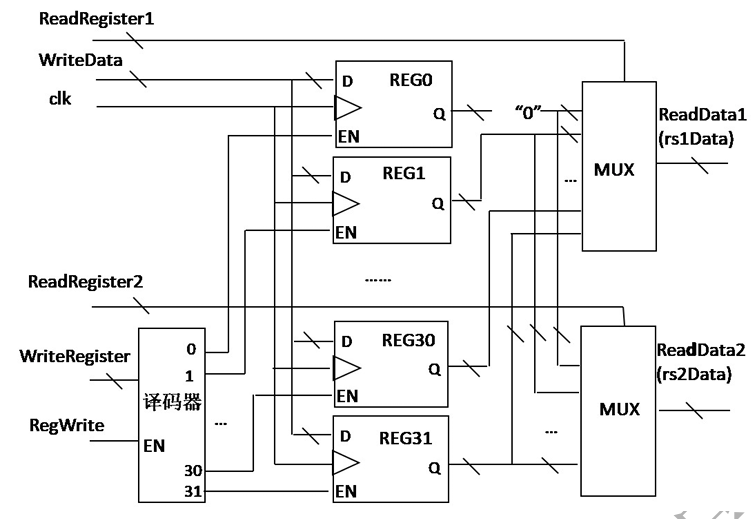
\includegraphics[width=0.8\textwidth]{e6.png}
    \caption{寄存器堆的原理框图}
\end{figure}

对于往寄存器里写数据，需要目标寄存器号（WriteRegister）、待写入数据（WriteData）、写允许信号（RegWrite）三个变量。图 30.8 中 5 位二进制译码器完成地址译码，其输出控制目标寄存器的写使能信号 EN，决定将数据 WriteData 写入哪个寄存器。

注意：用 Verilog HDL 设计描述寄存器堆时，用存储器变量定义 32 个 32 位寄存器更为方便。下面为描述寄存器堆核心语句。

\begin{lstlisting}[language=verilog]
reg [31:0]regs [31:0];//定义 32*32 存储器变量
assign ReadData1= (ReadRegister1 == 5'b0) ? 32'b0 : regs[ReadRegister1];//端口 1 数据读出
assign ReadData2= (ReadRegister2 == 5'b0) ? 32'b0 : regs[ReadRegister2];//端口 2 数据读出
always @ (posedge clk) if (RegWrite)regs[WriteRegister] <= WriteData; //数据写入
\end{lstlisting}

在流水线型 CPU 设计中，寄存器堆设计还应解决数据相关问题。当需三阶数据相关条件时，寄存器具有 Read After Write 特性：设计时，只需要在Figure 7
设计寄存器堆的基础上添加少量电路就可实现 Read After Write 特性，如图Figure 8所示。图中的 RBW\_Registers 模块就是实现图 30.8 的 Read Before Write 寄存器堆。图中转发检测电路的输出表达式为

\begin{align}
\text{rs1Sel} &= \text{RegWrite}\&\&(\text{WriteAddr}!=0)\&\&(\text{WriteAddr} ==\text{rs1Addr}) \tag{6.2.1} \\
\text{rs2Sel} &= \text{RegWrite}\&\&(\text{WriteAddr}!=0)\&\&(\text{WriteAddr} ==\text{rs2Addr}) \tag{6.2.2}
\end{align}

\begin{figure}[H]
    \centering
    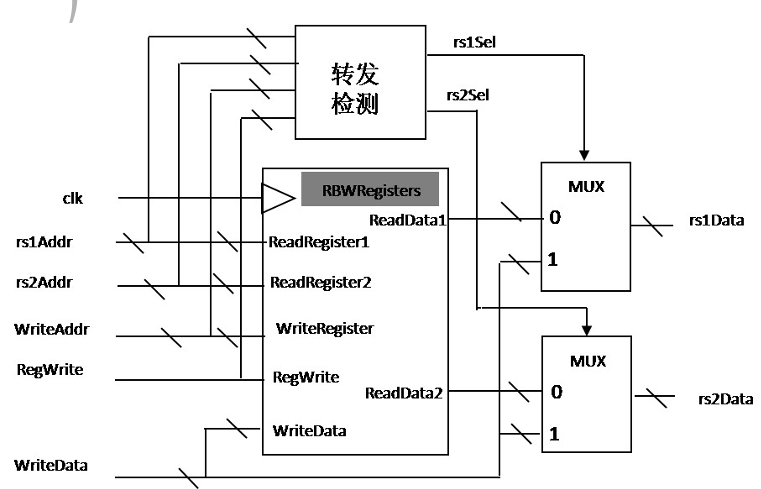
\includegraphics[width=0.9\textwidth]{e7.png}
    \caption{具有 Read After Write 特性寄存器堆的原理框图}
\end{figure}

\subsubsection{Verilog HDL代码与设计分析}

\textbf{(1) 寄存器阵列定义}

使用 32×32 位的存储器变量定义寄存器堆，简化设计实现。

\begin{lstlisting}[language=verilog]
//Register array definition
reg [31:0] regs [31:0];
\end{lstlisting}

\textbf{(2) 读端口逻辑}

读取端口通过多路选择器实现，特别处理 x0 寄存器，确保其值始终为 0。

\begin{lstlisting}[language=verilog]
//Read port logic with register 0 hardwired to zero
wire [31:0] ReadData1 = (rs1Addr_id == 5'b0) ? 32'b0 : regs[rs1Addr_id];
wire [31:0] ReadData2 = (rs2Addr_id == 5'b0) ? 32'b0 : regs[rs2Addr_id];
\end{lstlisting}

\textbf{(3) 写端口逻辑}

在时钟上升沿检测写使能信号，将数据写入目标寄存器。注意：即使写入 x0，硬件层面也会执行，但读取时 x0 始终返回 0。

\begin{lstlisting}[language=verilog]
//Write port logic on clock rising edge
always @(posedge clk) begin
    if (RegWrite_wb) begin
        regs[rdAddr_wb] <= RegWriteData_wb;
    end
end
\end{lstlisting}

\textbf{(4) RAW 冒险检测}

根据式 (6.2.1) 和式 (6.2.2)，检测读后写（Read After Write）数据冒险。当写使能有效、目标寄存器非 x0 且与读取地址相同时，触发转发。

\begin{lstlisting}[language=verilog]
//RAW hazard forwarding detection
wire rs1Sel = RegWrite_wb && (rdAddr_wb != 0) && (rdAddr_wb == rs1Addr_id);
wire rs2Sel = RegWrite_wb && (rdAddr_wb != 0) && (rdAddr_wb == rs2Addr_id);
\end{lstlisting}

\textbf{(5) 数据转发多路选择器}

根据冒险检测结果，选择输出数据源：若检测到 RAW 冒险，直接转发写入数据；否则输出寄存器读取值。

\begin{lstlisting}[language=verilog]
//Output MUX for Read After Write forwarding
assign rs1Data_id = rs1Sel ? RegWriteData_wb : ReadData1;
assign rs2Data_id = rs2Sel ? RegWriteData_wb : ReadData2;
\end{lstlisting}

\subsubsection{ModelSim仿真波形}
\begin{figure}[H]
    \centering
    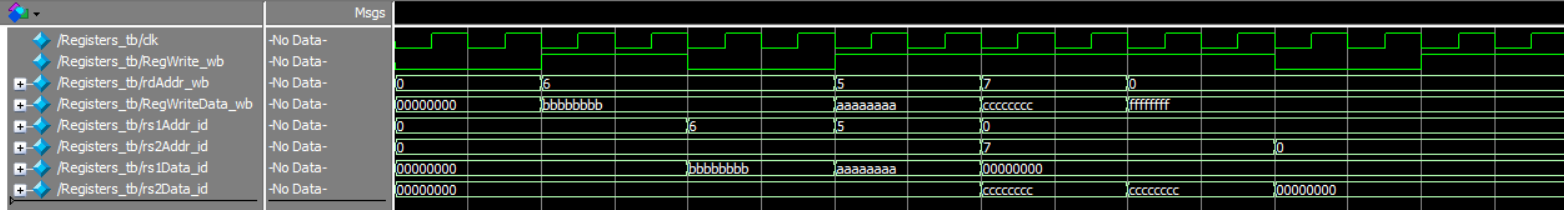
\includegraphics[width=1\textwidth]{Registers.png}
    \caption{Registers模块仿真波形}
\end{figure}

\subsubsection{实验结果分析}

通过 ModelSim 对 Registers 模块进行功能仿真，测试了寄存器读写和 RAW 转发功能。测试用例及预期结果如下：

\textbf{Test 1: 写入 x6 寄存器}

\begin{table}[H]
\centering
\begin{tabular}{|c|c|c|c|}
\hline
时间 & RegWrite\_wb & rdAddr\_wb & RegWriteData\_wb \\ \hline
20ns & 1 & 6 & 32'hBBBBBBBB \\ \hline
\end{tabular}
\caption{预期：x6 = 32'hBBBBBBBB}
\end{table}

\textbf{Test 2: 读取 x6 寄存器}

\begin{table}[H]
\centering
\begin{tabular}{|c|c|c|}
\hline
时间 & rs1Addr\_id & rs1Data\_id（预期） \\ \hline
40ns & 6 & 32'hBBBBBBBB \\ \hline
\end{tabular}
\caption{验证写入数据已正确存储}
\end{table}

\textbf{Test 3: RAW 转发测试 - rs1 端口}

\begin{table}[H]
\centering
\begin{tabular}{|c|c|c|c|c|}
\hline
时间 & RegWrite\_wb & rdAddr\_wb & rs1Addr\_id & rs1Data\_id（预期） \\ \hline
60ns & 1 & 5 & 5 & 32'hAAAAAAAA \\ \hline
\end{tabular}
\caption{同时写入和读取 x5，预期立即转发写入数据}
\end{table}

\textbf{Test 4: RAW 转发测试 - rs2 端口}

\begin{table}[H]
\centering
\begin{tabular}{|c|c|c|c|c|}
\hline
时间 & RegWrite\_wb & rdAddr\_wb & rs2Addr\_id & rs2Data\_id（预期） \\ \hline
80ns & 1 & 7 & 7 & 32'hCCCCCCCC \\ \hline
\end{tabular}
\caption{同时写入和读取 x7，预期立即转发写入数据}
\end{table}

\textbf{Test 5: 写入 x0 寄存器（应忽略）}

\begin{table}[H]
\centering
\begin{tabular}{|c|c|c|c|}
\hline
时间 & RegWrite\_wb & rdAddr\_wb & RegWriteData\_wb \\ \hline
100ns & 1 & 0 & 32'hFFFFFFFF \\ \hline
\end{tabular}
\caption{预期：x0 保持为 0（写入被忽略）}
\end{table}

\textbf{Test 6: 读取 x0 寄存器}

\begin{table}[H]
\centering
\begin{tabular}{|c|c|c|c|c|}
\hline
时间 & rs1Addr\_id & rs2Addr\_id & rs1Data\_id（预期） & rs2Data\_id（预期） \\ \hline
120ns & 0 & 0 & 32'h00000000 & 32'h00000000 \\ \hline
\end{tabular}
\caption{验证 x0 始终为 0}
\end{table}

\textbf{Test 7: x0 的 RAW 转发阻止}

\begin{table}[H]
\centering
\begin{tabular}{|c|c|c|c|c|}
\hline
时间 & RegWrite\_wb & rdAddr\_wb & rs1Addr\_id & rs1Data\_id（预期） \\ \hline
140ns & 1 & 0 & 0 & 32'h00000000 \\ \hline
\end{tabular}
\caption{同时写入和读取 x0，预期不转发，输出仍为 0}
\end{table}

仿真结果验证了以下功能：
\begin{enumerate}
    \item 寄存器读写功能正常，写入数据能正确存储并读出。
    \item RAW（Read After Write）转发机制有效，当同时读写同一寄存器时，能立即转发写入数据，避免数据冒险。
    \item x0 寄存器特殊处理正确，无论是否写入，读取时始终返回 0。
    \item 对 x0 的 RAW 转发被正确阻止（通过 rdAddr\_wb != 0 条件），保证 x0 的常量特性。
\end{enumerate}

\clearpage
\subsection{ID模块设计}
\subsubsection{设计原理}

指令译码模块的主要作用是从机器码中解析出指令，并根据解析结果输出各种控制信号。ID 模块主要由指令译码（Decode）、寄存器堆（Registers）、冒险检测、分支检测和加法器等组成。
其中，Decode 模块和 Registers 模块的设计已在前文设计完毕。
ID 模块的接口信息如表 30.3 所示。

\begin{figure}[H]
    \centering
    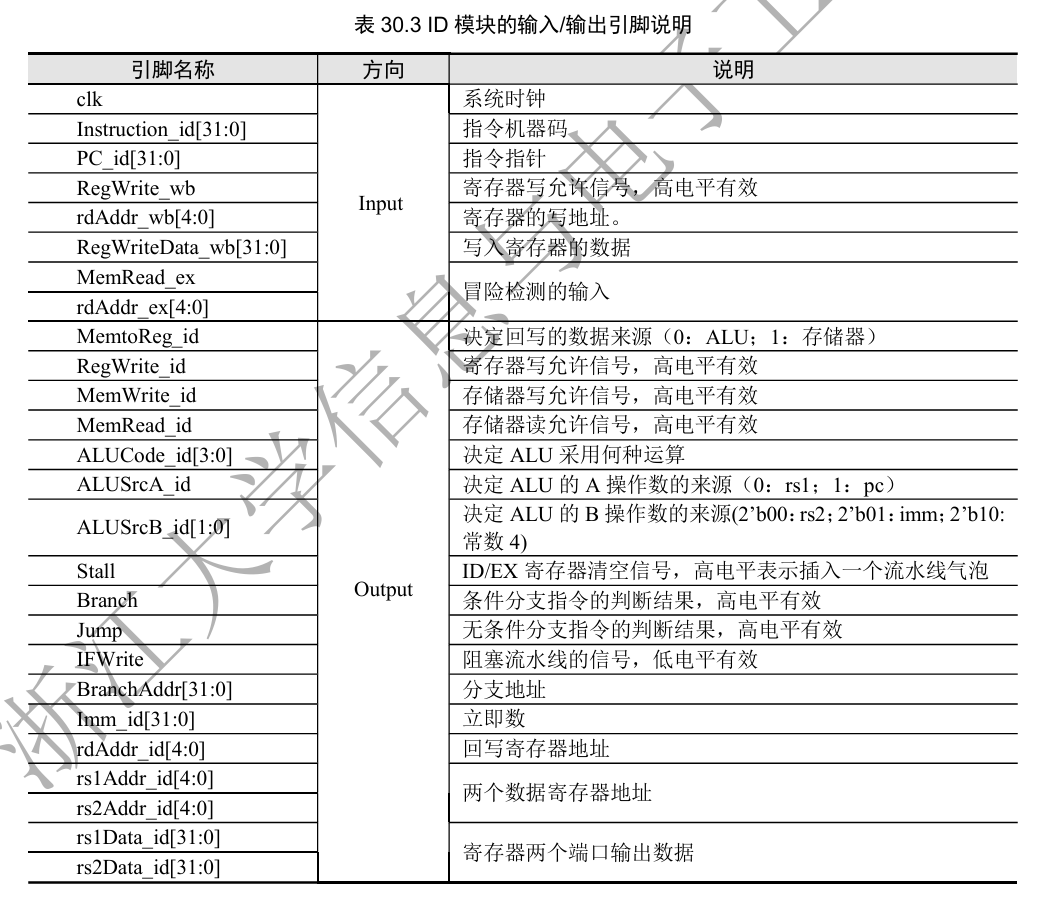
\includegraphics[width=0.9\textwidth]{e8.png}
\end{figure}

\textbf{(3) 分支检测（Branch Test）电路的设计}

分支检测电路主要用于判断分支条件是否成立，在 Verilog HDL 可以用比较运算符号 ">"、"==" 和 "<" 输运，但要注意符号数和无符号数的处理方法不同。在这里，我们用加法器来实现。

(1)用一个 32 位加法器完成 rs1Data+ ($\sim$rs2Data) +1（即 rs1Data-rs2Data），设结果为 sum [31:0]。

(2)确定比较运算的结果。对于比较运算来说，如果最高位不同，即 rs1Data [31]$\neq$rs2Data [31]，可根据 rs1Data [31]，rs2Data [31]决定比较结果，但是应注意符号数、无符号数的最高位 rs1Data [31]、rs2Data [31] 代表意义不同。若两数最高位相同，则两数之差不会溢出，所以比较运算结果可由两个操作数之差的符号位 sum[31]决定。

在符号数比较运算中，rs1Data<rs2Data 有以下两种情况：

a) rs1Data 为负数、rs2Data 为 0 或正数：rs1Data[31]\&\&($\sim$rs2Data[31])

b) rs1Data、rs2Data 符号相同，sum 为负：(rs1Data[31]$\wedge$rs2Data[31]) \&\& sum[31]

因此，符号数 rs1Data<rs2Data 比较运算结果为

\begin{equation}
\text{isLT} = \text{rs1Data[31]} \texttt{\&\&} (\sim \text{rs2Data[31]}) \texttt{||} (\text{rs1Data[31]} \oplus \text{rs2Data[31]}) \texttt{\&\&} \text{sum[31]}
\tag{6.3.3}
\end{equation}

同样地，无符号数比较算中，rs1Data<rs2Data 有以下两种情况：

a) rs1Data 最高位为 0、rs2Data 最高位为 1：($\sim$rs1Data[31] )\&\& rs2Data[31]

b) rs1Data、rs2Data 最高位相同，sum 为负：(rs1Data[31]$\wedge$rs2Data[31]) \&\& sum[31]

因此，无符号数比较运算结果为

\begin{equation}
\text{isLTU} = (\sim \text{rs1Data[31]}) \texttt{\&\&} \text{rs2Data[31]} \texttt{||} (\text{rs1Data[31]} \oplus \text{rs2Data[31]}) \texttt{\&\&} \text{sum[31]}
\tag{6.3.4}
\end{equation}

最后用数据选择器完成式(6.3.5)即可完成分支检测。

\begin{equation}
\text{Branch} = \begin{cases}
\sim (| \text{sum[31 : 0]}); & \text{SB\_type  \& \& (funct3 == beq\_funct3 )} \\
| \text{sum[31 : 0]}; & \text{SB\_type  \& \& (funct3 = bne\_funct3 )} \\
\text{isLT;} & \text{SB\_type  \& \&(funct3 = blt\_funct3 )} \\
\sim \text{ isLT ;} & \text{SB\_type  \& \& (funct3 = bge\_funct3 )} \\
\text{isLTU ;} & \text{SB\_type \& \& (funct3 = blu\_funct 3)} \\
\sim \text{isLTU ;} & \text{SB\_type  \& \& (funct3 = bgeu\_funct 3)} \\
0 & \text{others}
\end{cases}
\tag{6.3.5}
\end{equation}

\textbf{(4) 冒险检测功能电路（Hazard Detector）的设计}

由前面分析可知，冒险成立的条件为：

(1)上一条指令必须是 lw 指令（MemRead\_ex=1）;

(2)两条指令读写同一个寄存器（rdAddr\_ex=rs1Addr\_id 或 rdAddr\_ex=rs2Addr\_id）。

当冒险成立应清空 ID/EX 寄存器并且阻塞流水线 ID 级、IF 级流水线，所以有

\begin{align}
\text{Stall}&=\text{((rdAddr\_ex==rs1Addr\_id) || (rdAddr\_ex==rs2Addr\_id)) \&\&MemRead\_ex} \tag{6.3.6} \\
\text{IFWrite}&= \sim\text{Stall} \tag{6.3.7}
\end{align}

\subsubsection{Verilog HDL代码与设计分析}

\textbf{(1) 寄存器地址提取}

从指令的固定位域提取源寄存器和目标寄存器地址。

\begin{lstlisting}[language=verilog]
//Extract register addresses from instruction
assign rs1Addr_id = Instruction_id[19:15];
assign rs2Addr_id = Instruction_id[24:20];
assign rdAddr_id  = Instruction_id[11:7];
\end{lstlisting}

\textbf{(2) Registers 模块例化}

实例化寄存器堆模块，实现寄存器读写和 RAW 转发功能。接收 WB 阶段的写回信号，输出 ID 阶段的读取数据。

\begin{lstlisting}[language=verilog]
//Registers module: Register file with RAW hazard forwarding
Registers u_Registers (
    .clk(clk),
    .RegWrite_wb(RegWrite_wb),
    .rdAddr_wb(rdAddr_wb),
    .RegWriteData_wb(RegWriteData_wb),
    .rs1Addr_id(rs1Addr_id),
    .rs2Addr_id(rs2Addr_id),
    .rs1Data_id(rs1Data_id),
    .rs2Data_id(rs2Data_id)
);
\end{lstlisting}

\textbf{(3) Decode 模块例化}

实例化译码模块，根据指令生成各类控制信号、立即数和偏移量。

\begin{lstlisting}[language=verilog]
//Decode module: Instruction decode and control signal generation
Decode u_Decode (
    .Instruction(Instruction_id),
    .MemtoReg(MemtoReg_id),
    .RegWrite(RegWrite_id),
    .MemWrite(MemWrite_id),
    .MemRead(MemRead_id),
    .ALUCode(ALUCode_id),
    .ALUSrcA(ALUSrcA_id),
    .ALUSrcB(ALUSrcB_id),
    .Jump(Jump),
    .JALR(JALR_w),
    .Imm(Imm_id),
    .offset(offset_w)
);
\end{lstlisting}

\textbf{(4) Branch\_test 模块例化}

实例化分支测试模块，根据寄存器数据和指令功能码判断分支条件是否成立。

\begin{lstlisting}[language=verilog]
//Branch_test module: Branch condition evaluation
Branch_test u_Branch_test (
    .rs1Data_id(rs1Data_id),
    .rs2Data_id(rs2Data_id),
    .Instruction_id(Instruction_id),
    .Branch(Branch)
);
\end{lstlisting}

\textbf{(5) Hazard\_Detector 模块例化}

实例化冒险检测模块，根据式 (6.3.6) 和 (6.3.7) 检测 Load-Use 冒险，生成流水线阻塞信号。

\begin{lstlisting}[language=verilog]
//Hazard_Detector module: Load-use hazard detection and stall generation
Hazard_Detector u_Hazard_Detector (
    .MemRead_ex(MemRead_ex),
    .rdAddr_ex(rdAddr_ex),
    .rs1Addr_id(rs1Addr_id),
    .rs2Addr_id(rs2Addr_id),
    .Stall(Stall),
    .IFWrite(IFWrite)
);
\end{lstlisting}

\textbf{(6) 跳转地址计算}

根据当前 PC 值和偏移量计算跳转目标地址，用于分支和跳转指令。

\begin{lstlisting}[language=verilog]
//Jump address calculation
assign JumpAddr = PC_id + offset_w;
\end{lstlisting}

\subsubsection{ModelSim仿真波形}
\begin{figure}[H]
    \centering
    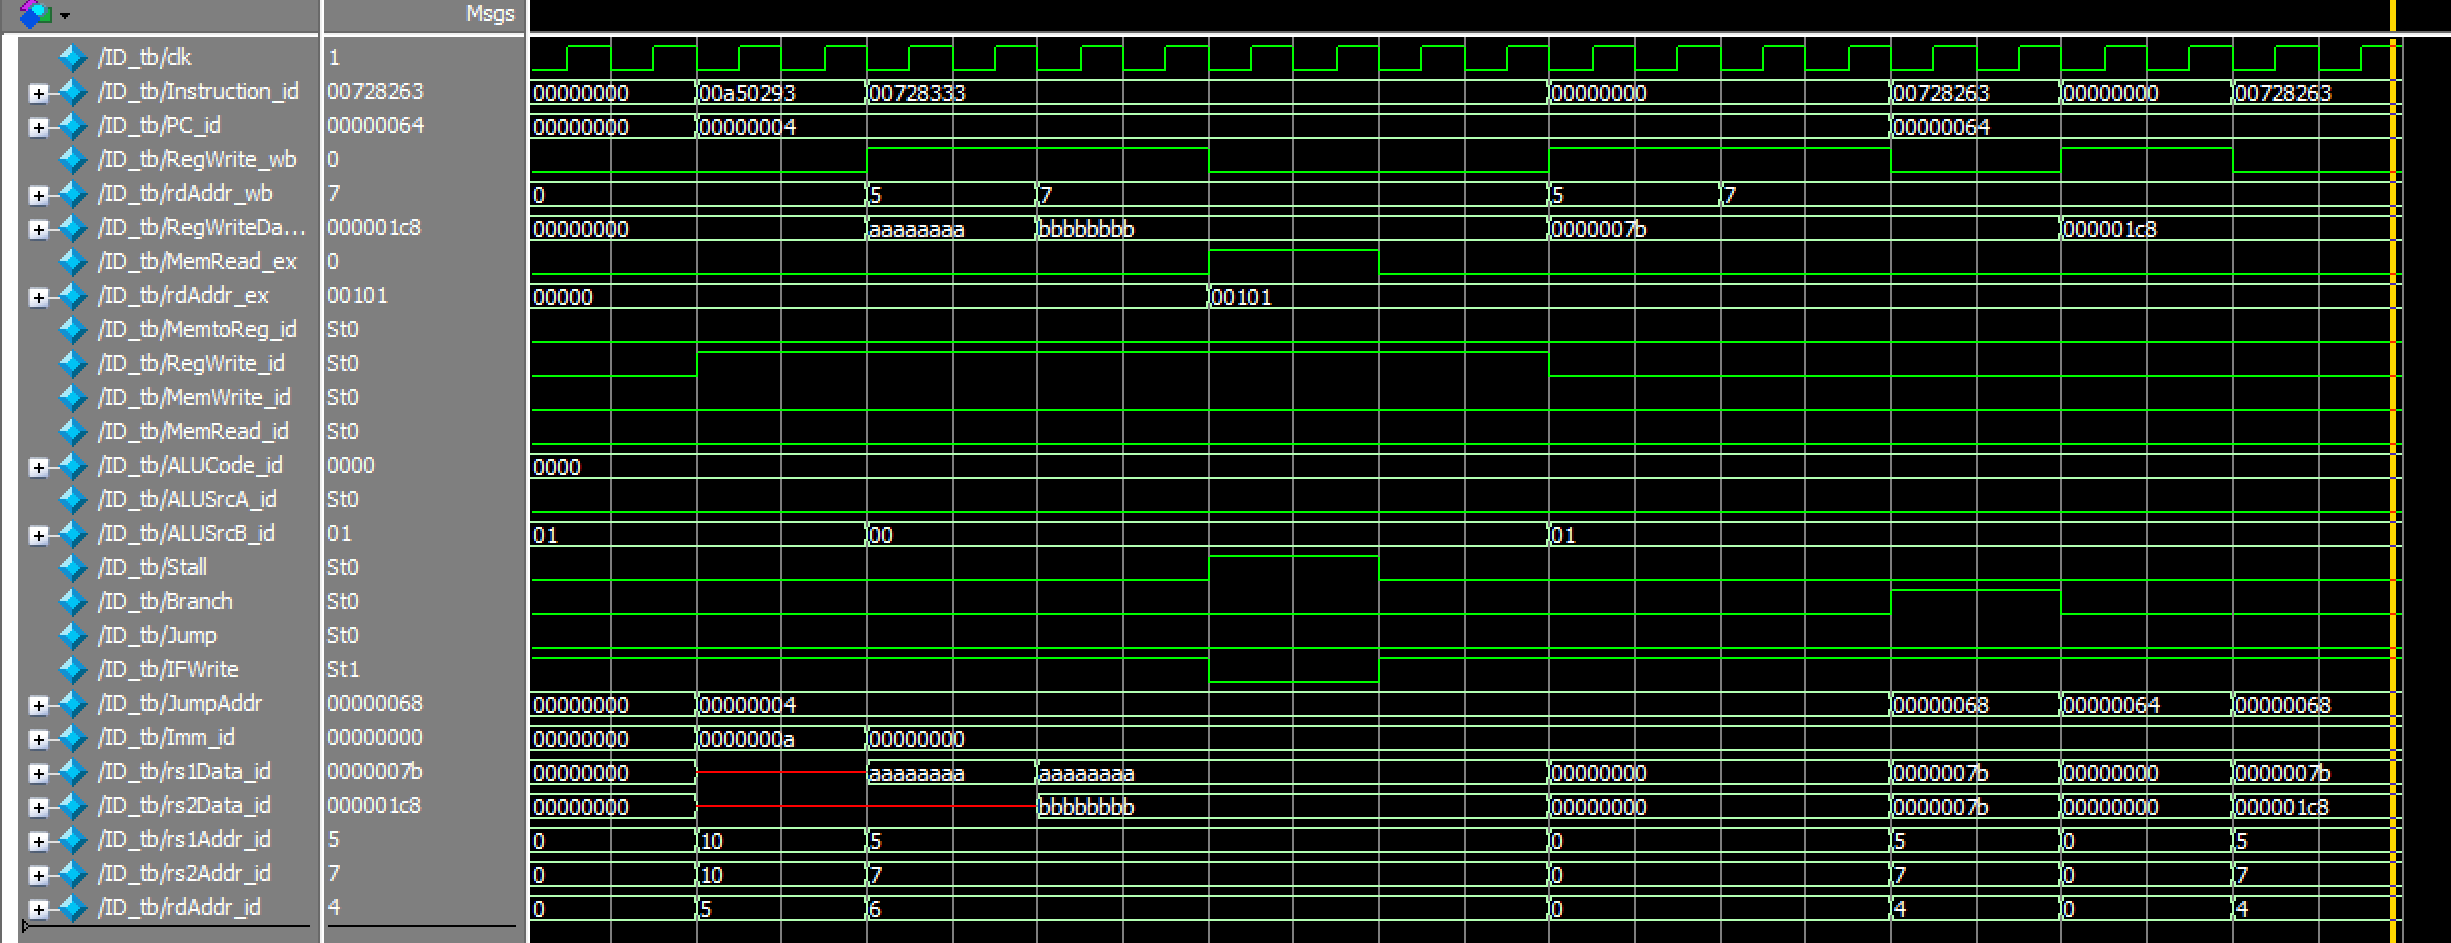
\includegraphics[width=1\textwidth]{ID.png}
    \caption{ID模块仿真波形}
\end{figure}

\subsubsection{实验结果分析}

通过 ModelSim 对 ID 模块进行综合功能仿真，测试了指令译码、寄存器读写、数据转发、冒险检测和分支判断等功能。测试用例及预期结果如下：

\textbf{Test 1: ADDI 指令译码（addi x5, x10, 10）}

\begin{table}[H]
\centering
\begin{tabular}{|c|c|c|c|c|c|c|}
\hline
Instruction & rs1Addr & rdAddr & Imm & RegWrite & MemRead & Stall \\ \hline
32'h00A50293 & 10 & 5 & 32'h0000000A & 1 & 0 & 0 \\ \hline
\end{tabular}
\caption{验证 I 型指令译码和立即数提取}
\end{table}

\textbf{Test 2: WB→ID RAW 转发测试（rs1 端口）}

指令：add x6, x5, x7，WB 阶段写入 x5 = 32'hAAAAAAAA

\begin{table}[H]
\centering
\begin{tabular}{|c|c|c|c|c|}
\hline
rs1Addr & rdAddr\_wb & RegWriteData\_wb & rs1Data\_id（预期） & Stall \\ \hline
5 & 5 & 32'hAAAAAAAA & 32'hAAAAAAAA & 0 \\ \hline
\end{tabular}
\caption{验证 WB 阶段数据立即转发到 ID 阶段 rs1}
\end{table}

\textbf{Test 3: WB→ID RAW 转发测试（rs2 端口）}

指令：add x6, x5, x7，WB 阶段写入 x7 = 32'hBBBBBBBB

\begin{table}[H]
\centering
\begin{tabular}{|c|c|c|c|c|}
\hline
rs2Addr & rdAddr\_wb & RegWriteData\_wb & rs2Data\_id（预期） & Stall \\ \hline
7 & 7 & 32'hBBBBBBBB & 32'hBBBBBBBB & 0 \\ \hline
\end{tabular}
\caption{验证 WB 阶段数据立即转发到 ID 阶段 rs2}
\end{table}

\textbf{Test 4: Load-Use 冒险检测}

EX 阶段：lw x5（MemRead\_ex=1, rdAddr\_ex=5），ID 阶段：add x6, x5, x7（rs1Addr=5）

\begin{table}[H]
\centering
\begin{tabular}{|c|c|c|c|c|}
\hline
MemRead\_ex & rdAddr\_ex & rs1Addr\_id & Stall（预期） & IFWrite（预期） \\ \hline
1 & 5 & 5 & 1 & 0 \\ \hline
\end{tabular}
\caption{检测到 Load-Use 冒险，流水线阻塞}
\end{table}

\textbf{Test 5: 冒险解除}

EX 阶段无 Load 指令（MemRead\_ex=0）

\begin{table}[H]
\centering
\begin{tabular}{|c|c|c|}
\hline
MemRead\_ex & Stall（预期） & IFWrite（预期） \\ \hline
0 & 0 & 1 \\ \hline
\end{tabular}
\caption{无冒险，流水线正常运行}
\end{table}

\textbf{Test 6-7: 分支测试准备}

向 x5 和 x7 分别写入 123（32'd123 = 32'h0000007B）

\begin{table}[H]
\centering
\begin{tabular}{|c|c|c|}
\hline
rdAddr\_wb & RegWriteData\_wb & 说明 \\ \hline
5 & 32'd123 & x5 = 123 \\ \hline
7 & 32'd123 & x7 = 123 \\ \hline
\end{tabular}
\caption{为分支测试准备相等的寄存器值}
\end{table}

\textbf{Test 8: 分支成立（BEQ x5, x7, offset）}

rs1Data = 123，rs2Data = 123，两值相等

\begin{table}[H]
\centering
\begin{tabular}{|c|c|c|c|c|}
\hline
Instruction & rs1Data & rs2Data & Branch（预期） & JumpAddr \\ \hline
32'h00728263 & 32'h7B & 32'h7B & 1 & PC + offset \\ \hline
\end{tabular}
\caption{BEQ 条件成立，分支跳转}
\end{table}

\textbf{Test 9: 分支测试准备（不等值）}

向 x7 写入 456（32'd456 = 32'h000001C8）

\begin{table}[H]
\centering
\begin{tabular}{|c|c|}
\hline
rdAddr\_wb & RegWriteData\_wb \\ \hline
7 & 32'd456 \\ \hline
\end{tabular}
\caption{x7 = 456，与 x5 不等}
\end{table}

\textbf{Test 10: 分支不成立（BEQ x5, x7, offset）}

rs1Data = 123，rs2Data = 456，两值不等

\begin{table}[H]
\centering
\begin{tabular}{|c|c|c|c|}
\hline
Instruction & rs1Data & rs2Data & Branch（预期） \\ \hline
32'h00728263 & 32'h7B & 32'h1C8 & 0 \\ \hline
\end{tabular}
\caption{BEQ 条件不成立，不跳转}
\end{table}

仿真结果验证了以下功能：
\begin{enumerate}
    \item \textbf{指令译码}：正确提取寄存器地址、立即数和偏移量，生成各类控制信号。
    \item \textbf{寄存器读写}：Registers 模块正常工作，支持同时读写操作。
    \item \textbf{WB→ID 数据转发}：当 WB 阶段写入的寄存器与 ID 阶段读取的寄存器相同时，能立即转发数据，避免数据冒险。
    \item \textbf{Load-Use 冒险检测}：正确检测 EX 阶段 Load 指令与 ID 阶段指令的寄存器依赖，及时插入流水线气泡（Stall=1, IFWrite=0）。
    \item \textbf{分支条件判断}：Branch\_test 模块正确比较寄存器值，BEQ 指令在操作数相等时 Branch=1，不等时 Branch=0。
    \item \textbf{跳转地址计算}：JumpAddr 正确计算为 PC + offset。
\end{enumerate}

综合测试表明，ID 模块能够正确完成指令译码阶段的所有功能，包括控制信号生成、数据读取、冒险检测和分支判断，为流水线 CPU 的正常运行提供了保障。

\clearpage
\subsection{ALU模块设计}
\subsubsection{设计原理}

算术逻辑运算单元（ALU）提供 CPU 的基本运算能力，如加、减、与、或、比较、移位等。具体而言，ALU 输入为两个操作数 A、B 和控制信号 ALUCode，由控制信号 ALUCode 决定采用何种运算，运算结果为 ALUResult。整理表 30.5 所示的 ALUCode 的功能表，可得到 ALU 的功能表，如表 30.8 所示。

\begin{figure}[H]
    \centering
    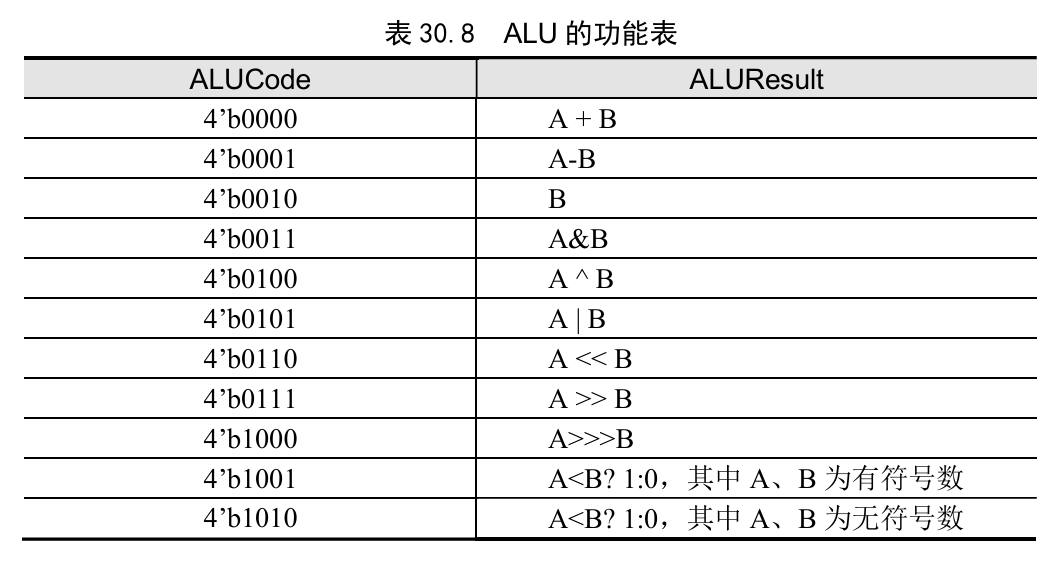
\includegraphics[width=0.9\textwidth]{e9.png}

\end{figure}

如表 30.8 所示，ALU 需执行多种运算。为了提高运算速度，本设计可同时进行各种运算，再根据 ALUCode 信号选出所需结果。ALU 的基本结构如图30.10所示。

\begin{figure}[H]
    \centering
    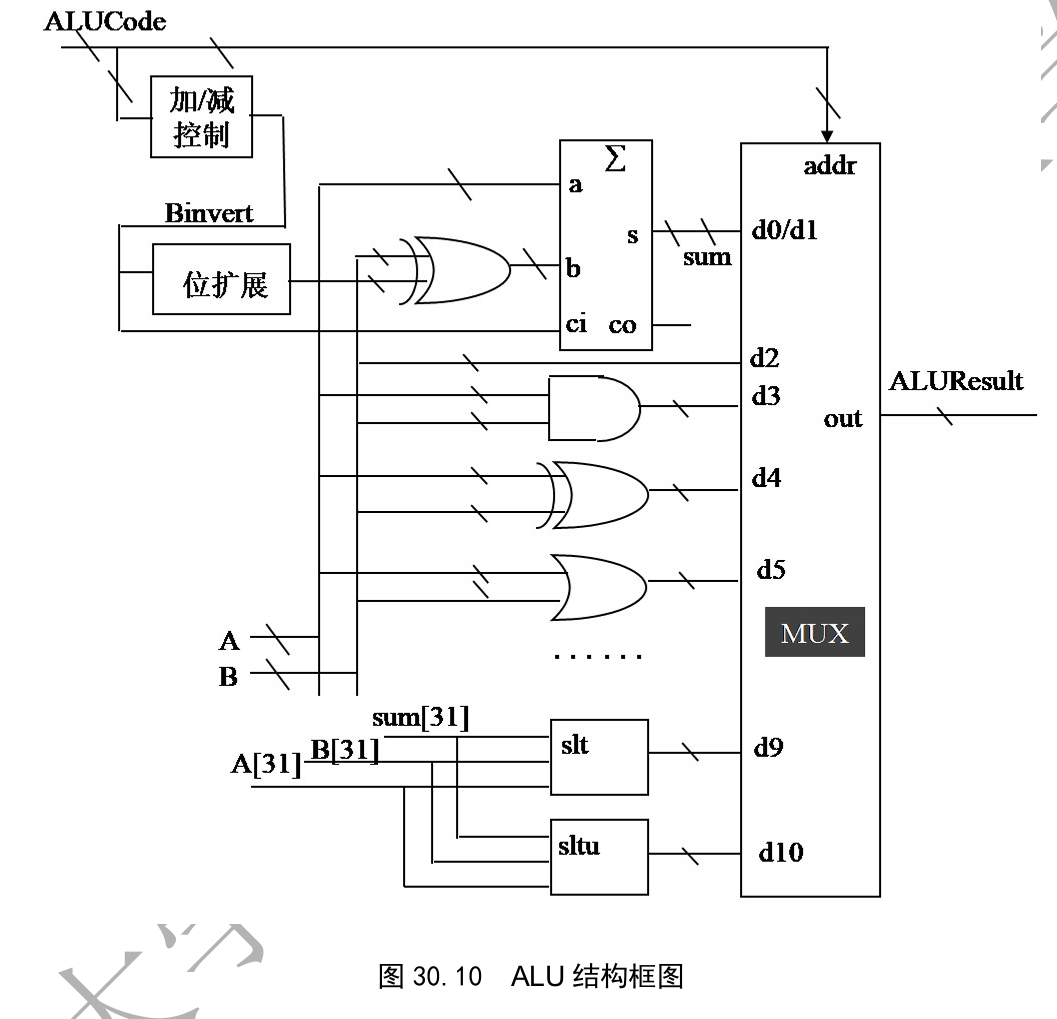
\includegraphics[width=0.9\textwidth]{e10.png}
\end{figure}

\textbf{(1)加、减电路的设计考虑}

减法、比较（slt、slu）均可用加法器和必要辅助电路来实现。图30.10中的 Binvert 信号控制加减运算。若 Binvert 信号为低电平，则实现加法运算 sum=A+B；若 Binvert 信号为高电平，则电路为减法运算 sum=A-B。除此外，减法、比较和分支指令都应使电路工作在减法状态，所以：

\begin{equation}
\text{Binvert}=(\text{ALUCode}==0)
\tag{6.4.1}
\end{equation}

最后要强调的是，32 位加法器的运算速度决定了 RISC-V 微处理器的时钟信号频率的高低，因此设计一个高速的 32 位加法器尤为重要。32 位加法器可采用实验 8 介绍的进位选择加法器。

\textbf{(2)比较电路的设计考虑}

比较电路的设计方法已在分支检测电路介绍，参考式(6.3.3)和式(6.3.4)可确定 slt 和 slu 两条件的比较结果。

\textbf{(3)算术右移运算电路的设计考虑}

算术右移对有符号数而言，移出的高位补符号位而不是 0。每右移一位相当于除以 2。例如，有符号数负数 10100100(-76)算术右移两位结果为 11101001(-19)，正数 01100111(103)算术右移一位结果为 00110011(51)。

Verilog HDL 的算术右移的运算符是 ">>>"。要实现算术右移应注意，被移位的对象必须定义是 reg 类型，但是在 sra 指令，被移位的对象操作数 A 为输入信号，不能定义为 reg 类型。因此，必须引入 reg 类型中间变量 A\_reg，相应的 Verilog HDL 语句为

\begin{lstlisting}[language=verilog]
reg signed[31:0] A_reg;
always @(*) begin A_reg=A; end
\end{lstlisting}

引入 reg 类型的中间变量 A\_reg 后，就可对 A\_reg 进行算术右移操作。

\subsubsection{Verilog HDL代码与设计分析}

\textbf{(1) ALU 操作码参数定义}

定义 11 种 ALU 运算对应的操作码，便于代码可读性和维护。

\begin{lstlisting}[language=verilog]
//Parameters for ALU operations
parameter alu_add  = 4'b0000;
parameter alu_sub  = 4'b0001;
parameter alu_lui  = 4'b0010;
parameter alu_and  = 4'b0011;
parameter alu_xor  = 4'b0100;
parameter alu_or   = 4'b0101;
parameter alu_sll  = 4'b0110;
parameter alu_srl  = 4'b0111;
parameter alu_sra  = 4'b1000;
parameter alu_slt  = 4'b1001;
parameter alu_sltu = 4'b1010;
\end{lstlisting}

\textbf{(2) 加减法控制逻辑}

根据式 (6.4.1)，当 ALUCode 为 sub、slt 或 sltu 时，Binvert=1 实现减法。通过 XOR 门对 B 取反，结合进位输入实现补码减法。

\begin{lstlisting}[language=verilog]
//Add/Sub control: Binvert=1 for sub, slt, sltu
assign Binvert = (ALUCode == alu_sub) || (ALUCode == alu_slt) || (ALUCode == alu_sltu);

//B input XOR gate
assign B_inv = B ^ {32{Binvert}}; 

//32-bit Adder instantiation
adder_32bits u_adder (
    .a(A),
    .b(B_inv),
    .ci(Binvert),
    .s(sum),
    .co(co_unused)
);
\end{lstlisting}

\textbf{(3) 逻辑运算单元}

并行实现与、或、异或运算，为最终多路选择器提供输入。

\begin{lstlisting}[language=verilog]
//Logic operations
assign d3 = A & B;  // AND
assign d4 = A ^ B;  // XOR
assign d5 = A | B;  // OR
\end{lstlisting}

\textbf{(4) 移位运算单元}

实现逻辑左移、逻辑右移和算术右移。算术右移使用有符号类型的中间变量，按式 (6.4.1) 设计考虑实现。

\begin{lstlisting}[language=verilog]
//Shift operations
assign d6 = A << B[4:0];   // SLL
assign d7 = A >> B[4:0];   // SRL

reg signed [31:0] A_signed;
always @(*) A_signed = A;
assign d8 = A_signed >>> B[4:0];  // SRA
\end{lstlisting}

\textbf{(5) 比较运算单元}

根据前文分支检测电路的设计方法，实现有符号比较（slt）和无符号比较（sltu）。比较结果为 1 位，扩展为 32 位输出。

\begin{lstlisting}[language=verilog]
//Comparators
wire slt_bit  = (A[31] & ~B[31]) | ((A[31] ~^ B[31]) & sum[31]);
wire sltu_bit = (~A[31] & B[31]) | ((A[31] ~^ B[31]) & sum[31]);

assign d9  = {31'd0, slt_bit};   // SLT
assign d10 = {31'd0, sltu_bit};  // SLTU
\end{lstlisting}

\textbf{(6) 最终结果选择器}

根据 ALUCode 从 11 个并行运算结果中选择对应的输出，实现多路选择功能。

\begin{lstlisting}[language=verilog]
//Final MUX
always @(*) case (ALUCode)
    alu_add:  ALUResult = d0;
    alu_sub:  ALUResult = d1;
    alu_lui:  ALUResult = d2;
    alu_and:  ALUResult = d3;
    alu_xor:  ALUResult = d4;
    alu_or:   ALUResult = d5;
    alu_sll:  ALUResult = d6;
    alu_srl:  ALUResult = d7;
    alu_sra:  ALUResult = d8;
    alu_slt:  ALUResult = d9;
    alu_sltu: ALUResult = d10;
    default:  ALUResult = 32'hxxxxxxxx;
endcase
\end{lstlisting}

\subsubsection{ModelSim仿真波形}

\begin{figure}[H]
    \centering
    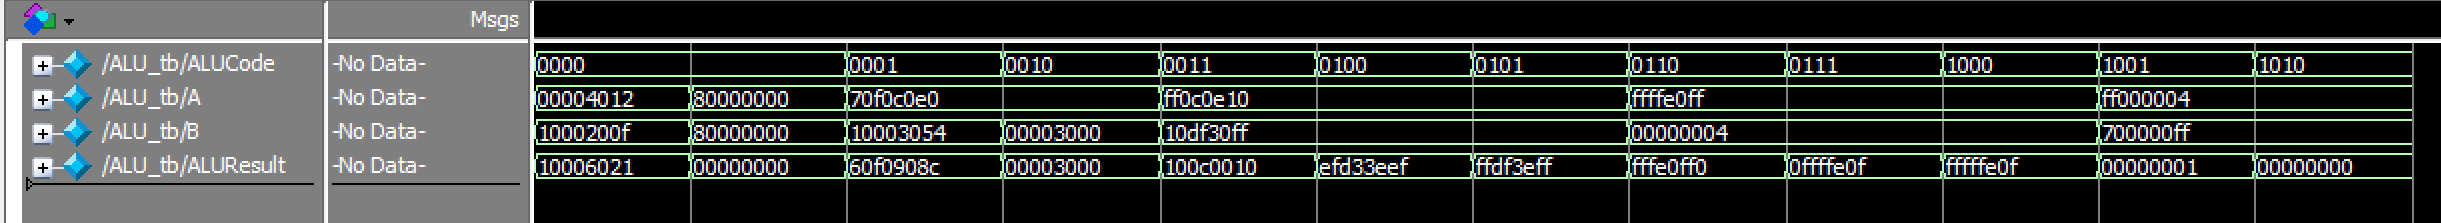
\includegraphics[width=1\textwidth]{ALU.png}
    \caption{ALU模块仿真波形}
\end{figure}

\subsubsection{实验结果分析}

通过 ModelSim 对 ALU 模块进行功能仿真，测试了 11 种算术逻辑运算，验证各运算单元的正确性。测试用例及预期结果如下：

\textbf{Test 1: ADD 运算（正常加法）}

\begin{table}[H]
\centering
\begin{tabular}{|c|c|c|c|}
\hline
ALUCode & A & B & ALUResult（预期） \\ \hline
4'b0000 & 32'h00004012 & 32'h1000200F & 32'h10006021 \\ \hline
\end{tabular}
\caption{验证普通加法运算}
\end{table}

\textbf{Test 2: ADD 运算（溢出测试）}

\begin{table}[H]
\centering
\begin{tabular}{|c|c|c|c|}
\hline
ALUCode & A & B & ALUResult（预期） \\ \hline
4'b0000 & 32'h80000000 & 32'h80000000 & 32'h00000000 \\ \hline
\end{tabular}
\caption{验证加法溢出（有符号负数相加）}
\end{table}

\textbf{Test 3: SUB 运算}

\begin{table}[H]
\centering
\begin{tabular}{|c|c|c|c|}
\hline
ALUCode & A & B & ALUResult（预期） \\ \hline
4'b0001 & 32'h70F0C0E0 & 32'h10003054 & 32'h60ED908C \\ \hline
\end{tabular}
\caption{验证减法运算（A - B）}
\end{table}

\textbf{Test 4: LUI 运算}

\begin{table}[H]
\centering
\begin{tabular}{|c|c|c|c|}
\hline
ALUCode & A & B & ALUResult（预期） \\ \hline
4'b0010 & 32'h70F0C0E0 & 32'h00003000 & 32'h00003000 \\ \hline
\end{tabular}
\caption{验证 LUI 指令（输出 B 值）}
\end{table}

\textbf{Test 5: AND 运算}

\begin{table}[H]
\centering
\begin{tabular}{|c|c|c|c|}
\hline
ALUCode & A & B & ALUResult（预期） \\ \hline
4'b0011 & 32'hFF0C0E10 & 32'h10DF30FF & 32'h100C0010 \\ \hline
\end{tabular}
\caption{验证按位与运算}
\end{table}

\textbf{Test 6: XOR 运算}

\begin{table}[H]
\centering
\begin{tabular}{|c|c|c|c|}
\hline
ALUCode & A & B & ALUResult（预期） \\ \hline
4'b0100 & 32'hFF0C0E10 & 32'h10DF30FF & 32'hEFD33EEF \\ \hline
\end{tabular}
\caption{验证按位异或运算}
\end{table}

\textbf{Test 7: OR 运算}

\begin{table}[H]
\centering
\begin{tabular}{|c|c|c|c|}
\hline
ALUCode & A & B & ALUResult（预期） \\ \hline
4'b0101 & 32'hFF0C0E10 & 32'h10DF30FF & 32'hFFDF3EFF \\ \hline
\end{tabular}
\caption{验证按位或运算}
\end{table}

\textbf{Test 8: SLL 运算（逻辑左移）}

\begin{table}[H]
\centering
\begin{tabular}{|c|c|c|c|}
\hline
ALUCode & A & B & ALUResult（预期） \\ \hline
4'b0110 & 32'hFFFFE0FF & 32'h00000004 & 32'hFFFE0FF0 \\ \hline
\end{tabular}
\caption{验证逻辑左移 4 位}
\end{table}

\textbf{Test 9: SRL 运算（逻辑右移）}

\begin{table}[H]
\centering
\begin{tabular}{|c|c|c|c|}
\hline
ALUCode & A & B & ALUResult（预期） \\ \hline
4'b0111 & 32'hFFFFE0FF & 32'h00000004 & 32'h0FFFFE0F \\ \hline
\end{tabular}
\caption{验证逻辑右移 4 位（高位补 0）}
\end{table}

\textbf{Test 10: SRA 运算（算术右移）}

\begin{table}[H]
\centering
\begin{tabular}{|c|c|c|c|}
\hline
ALUCode & A & B & ALUResult（预期） \\ \hline
4'b1000 & 32'hFFFFE0FF & 32'h00000004 & 32'hFFFFFE0F \\ \hline
\end{tabular}
\caption{验证算术右移 4 位（高位补符号位 1）}
\end{table}

\textbf{Test 11: SLT 运算（有符号比较）}

\begin{table}[H]
\centering
\begin{tabular}{|c|c|c|c|}
\hline
ALUCode & A & B & ALUResult（预期） \\ \hline
4'b1001 & 32'hFF000004 & 32'h700000FF & 32'h00000001 \\ \hline
\end{tabular}
\caption{A 为负数，B 为正数，A < B，结果为 1}
\end{table}

\textbf{Test 12: SLTU 运算（无符号比较）}

\begin{table}[H]
\centering
\begin{tabular}{|c|c|c|c|}
\hline
ALUCode & A & B & ALUResult（预期） \\ \hline
4'b1010 & 32'hFF000004 & 32'h700000FF & 32'h00000000 \\ \hline
\end{tabular}
\caption{无符号比较：A > B，结果为 0}
\end{table}

仿真结果验证了以下功能：
\begin{enumerate}
    \item \textbf{加减法运算}：正确实现加法和减法，包括溢出情况的处理。
    \item \textbf{逻辑运算}：AND、OR、XOR 按位逻辑运算结果正确。
    \item \textbf{移位运算}：逻辑左移（SLL）、逻辑右移（SRL）和算术右移（SRA）功能正确，SRA 正确保持符号位。
    \item \textbf{比较运算}：有符号比较（SLT）和无符号比较（SLTU）能正确判断大小关系，符号位处理正确。
    \item \textbf{LUI 指令}：正确输出 B 操作数（立即数）。
    \item \textbf{并行运算结构}：所有运算单元并行工作，通过多路选择器快速输出结果，提高运算速度。
\end{enumerate}

综合测试表明，ALU 模块能够正确执行 RISC-V 指令集要求的全部算术逻辑运算，为 CPU 提供了可靠的运算支持。

\clearpage
\subsection{EX模块设计}
\subsubsection{设计原理}

执行模块主要由 ALU 子模块、数据前推电路（Forwarding）及旁干数据选择器组成。执行模块的接口信息如表 30.7 所示。
其中，ALU模块已在上文设计完毕

\begin{figure}[H]
    \centering
    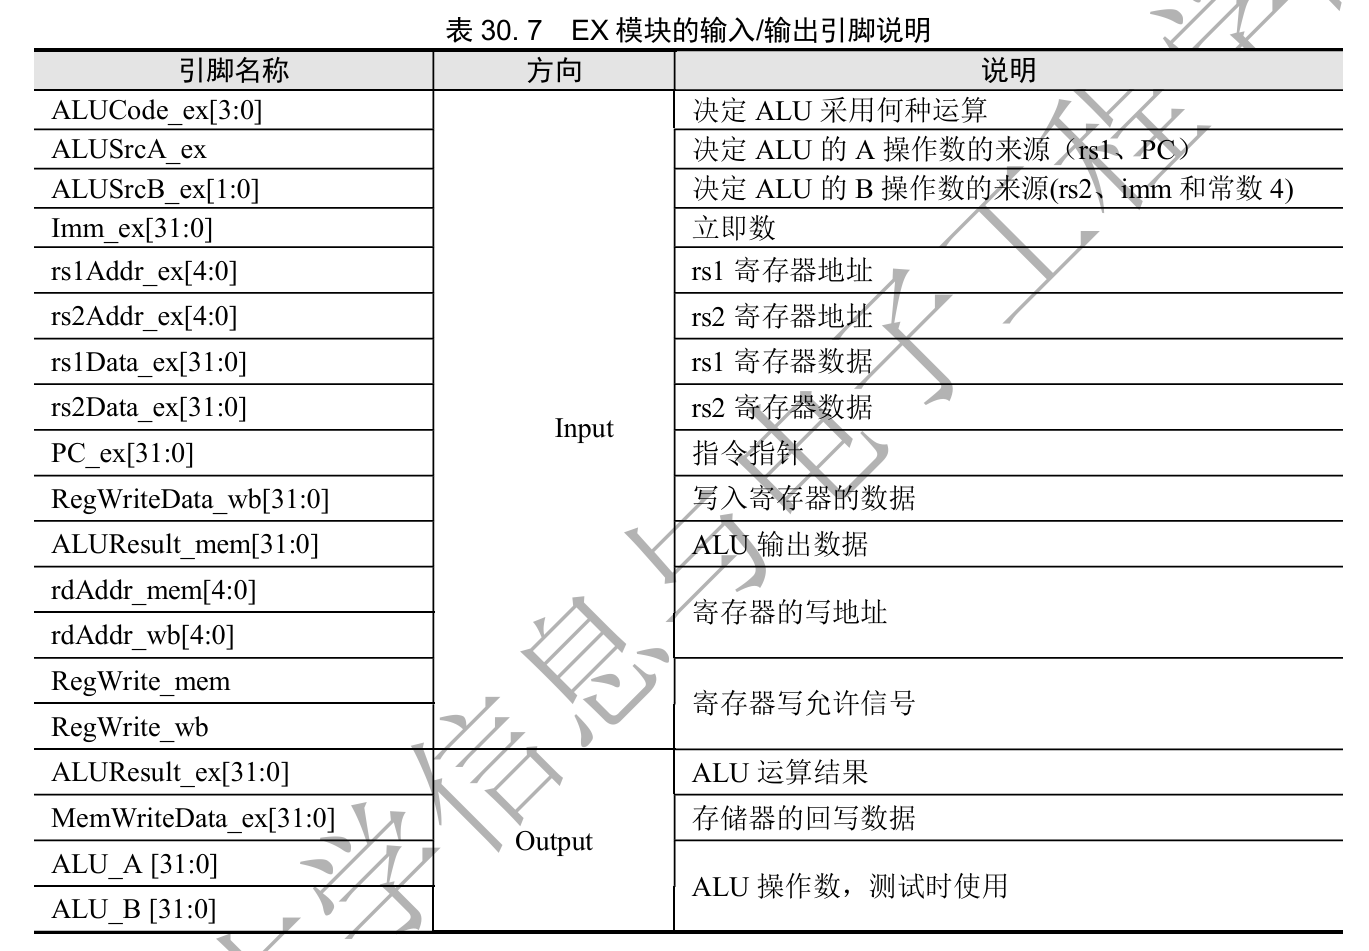
\includegraphics[width=0.9\textwidth]{e11.png}
\end{figure}

\textbf{(2) 数据前推电路的设计}

操作数 A 和 B 分别由数据选择器决定，数据选择器地址信号 ForwardA、ForwardB 的含义如表 30.9 所示。

\begin{figure}[H]
    \centering
    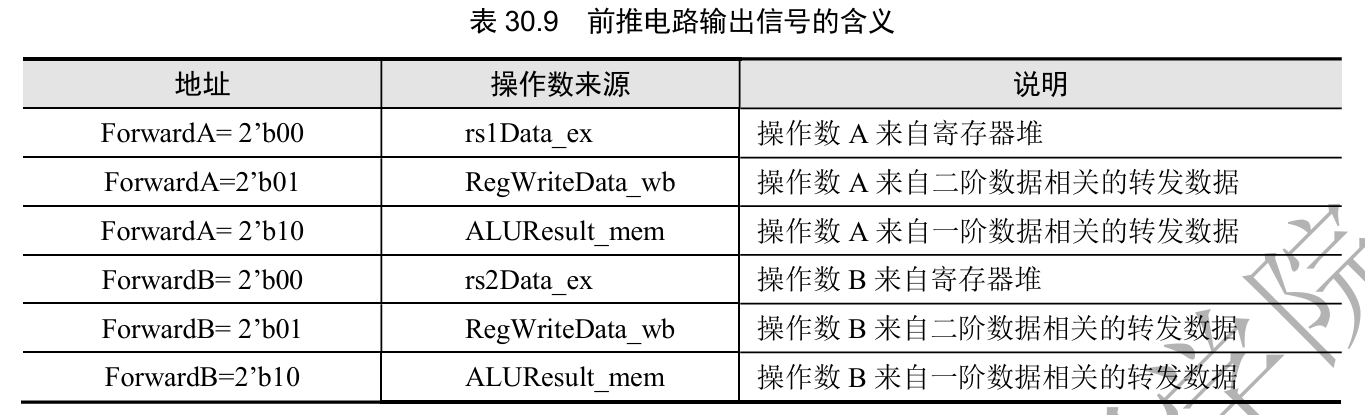
\includegraphics[width=0.9\textwidth]{e12.png}
\end{figure}

由前面介绍的一、二阶数据相关判断条件，不难得到

\begin{equation}
\begin{cases}
\text{ForwardA[0]} = \text{RegWrite\_wb} \texttt{\&\&} (\text{rdAddr\_wb}!= 0) \texttt{\&\&} \\
\qquad\qquad\qquad (\text{rdAddr\_mem}!= \text{rs1Addr\_ex}) \texttt{\&\&} \\
\qquad\qquad\qquad (\text{rdAddr\_wb} == \text{rs1Addr\_ex}) \\
\text{ForwardA[1]} = \text{RegWrite\_mem} \texttt{\&\&} (\text{rdAddr\_mem}!= 0) \texttt{\&\&} \\
\qquad\qquad\qquad (\text{rdAddr\_mem} == \text{rs1Addr\_ex})
\end{cases}
\tag{6.5.1}
\end{equation}

\begin{equation}
\begin{cases}
\text{ForwardB[0]} = \text{RegWrite\_wb} \texttt{\&\&} (\text{rdAddr\_wb}!= 0) \texttt{\&\&} \\
\qquad\qquad\qquad (\text{rd\_mem}!= \text{rs2Addr\_ex}) \texttt{\&\&} \\
\qquad\qquad\qquad (\text{rdAddr\_wb} == \text{rs2Addr\_ex}) \\
\text{ForwardB[1]} = \text{RegWrite\_mem} \texttt{\&\&} (\text{rdAddr\_mem}!= 0) \texttt{\&\&} \\
\qquad\qquad\qquad (\text{rdAddr\_mem} == \text{rs2Addr\_ex})
\end{cases}
\tag{6.5.2}
\end{equation}

\subsubsection{Verilog HDL代码与设计分析}

\textbf{(1) 模块接口定义}

EX 模块集成了 ALU 和 Forwarding 单元，包含来自 ID/EX 寄存器的控制信号、数据通路，以及来自 MEM 和 WB 阶段的前推数据。

\begin{lstlisting}[language=verilog]
module EX(
    // Inputs from ID/EX Register
    input [3:0] ALUCode_ex,
    input ALUSrcA_ex,
    input [1:0] ALUSrcB_ex,
    input [31:0] Imm_ex,
    input [4:0]  rs1Addr_ex,
    input [4:0]  rs2Addr_ex,
    input [31:0] rs1Data_ex,
    input [31:0] rs2Data_ex,
    input [31:0] PC_ex,
    // Inputs from WB Stage (Forwarding)
    input [31:0] RegWriteData_wb,
    input [4:0] rdAddr_wb,
    input RegWrite_wb,
    // Inputs from MEM Stage (Forwarding)
    input [31:0] ALUResult_mem,
    input [4:0] rdAddr_mem,
    input RegWrite_mem,
    // Outputs to EX/MEM Register
    output [31:0] ALUResult_ex,
    output [31:0] MemWriteData_ex,
    // Outputs for Debugging
    output [31:0] ALU_A,
    output [31:0] ALU_B
);
\end{lstlisting}

\textbf{(2) 内部信号定义}

定义前推控制信号和多路选择器输出，用于连接 Forwarding 模块和操作数选择逻辑。

\begin{lstlisting}[language=verilog]
// Internal Wires
wire [1:0] ForwardA_w;
wire [1:0] ForwardB_w;
wire [31:0] ForwardA_mux_out;
wire [31:0] ForwardB_mux_out;
\end{lstlisting}

\textbf{(3) Forwarding 模块例化}

根据式 (6.5.1) 和式 (6.5.2)，Forwarding 模块检测 EX-MEM 和 MEM-WB 数据相关，生成前推控制信号。

\begin{lstlisting}[language=verilog]
// Forwarding module: Detects EX and MEM hazards
Forwarding u_Forwarding (
    .RegWrite_mem(RegWrite_mem),
    .rdAddr_mem(rdAddr_mem),
    .RegWrite_wb(RegWrite_wb),
    .rdAddr_wb(rdAddr_wb),
    .rs1Addr_ex(rs1Addr_ex),
    .rs2Addr_ex(rs2Addr_ex),
    .ForwardA(ForwardA_w),
    .ForwardB(ForwardB_w)
);
\end{lstlisting}

\textbf{(4) ALU 模块例化}

调用前面设计的 ALU 模块执行算术逻辑运算，输入为经过前推和多路选择后的操作数。

\begin{lstlisting}[language=verilog]
// ALU module: Performs the calculation
ALU u_ALU (
    .ALUResult(ALUResult_ex),
    .ALUCode(ALUCode_ex),
    .A(ALU_A),
    .B(ALU_B)
);
\end{lstlisting}

\textbf{(5) ALU 操作数 A 选择逻辑}

第一级多路选择器根据 ForwardA 信号从 rs1Data、WB 前推数据、MEM 前推数据中选择。第二级根据 ALUSrcA 决定使用 PC 还是前推后的 rs1 数据。

\begin{lstlisting}[language=verilog]
// ALU Operand A MUX
// Selects between rs1Data, forwarded WB data, or forwarded MEM data
assign ForwardA_mux_out = (ForwardA_w == 2'b00) ? rs1Data_ex :
                          (ForwardA_w == 2'b01) ? RegWriteData_wb :
                          (ForwardA_w == 2'b10) ? ALUResult_mem :
                          rs1Data_ex;

// Selects final ALU_A input between PC or forwarded rs1Data
assign ALU_A = ALUSrcA_ex ? PC_ex : ForwardA_mux_out;
\end{lstlisting}

\textbf{(6) ALU 操作数 B 选择逻辑}

第一级多路选择器根据 ForwardB 信号从 rs2Data、WB 前推数据、MEM 前推数据中选择。第二级根据 ALUSrcB 决定使用前推后的 rs2 数据、立即数或常数 4。

\begin{lstlisting}[language=verilog]
// ALU Operand B MUX
// Selects between rs2Data, forwarded WB data, or forwarded MEM data
assign ForwardB_mux_out = (ForwardB_w == 2'b00) ? rs2Data_ex :
                          (ForwardB_w == 2'b01) ? RegWriteData_wb :
                          (ForwardB_w == 2'b10) ? ALUResult_mem :
                          rs2Data_ex;

// Selects final ALU_B input between forwarded rs2Data, immediate, or constant 4
assign ALU_B = (ALUSrcB_ex == 2'b00) ? ForwardB_mux_out :
               (ALUSrcB_ex == 2'b01) ? Imm_ex :
               (ALUSrcB_ex == 2'b10) ? 32'd4 :
               Imm_ex;
\end{lstlisting}

\textbf{(7) 存储器写数据输出}

对于 SW 指令，需要将前推后的 rs2 数据传递到 MEM 阶段写入存储器。

\begin{lstlisting}[language=verilog]
// Data to be written to memory (for SW instruction)
// This is the forwarded rs2 data
assign MemWriteData_ex = ForwardB_mux_out;
\end{lstlisting}

\subsubsection{ModelSim仿真波形}
\begin{figure}[H]
    \centering
    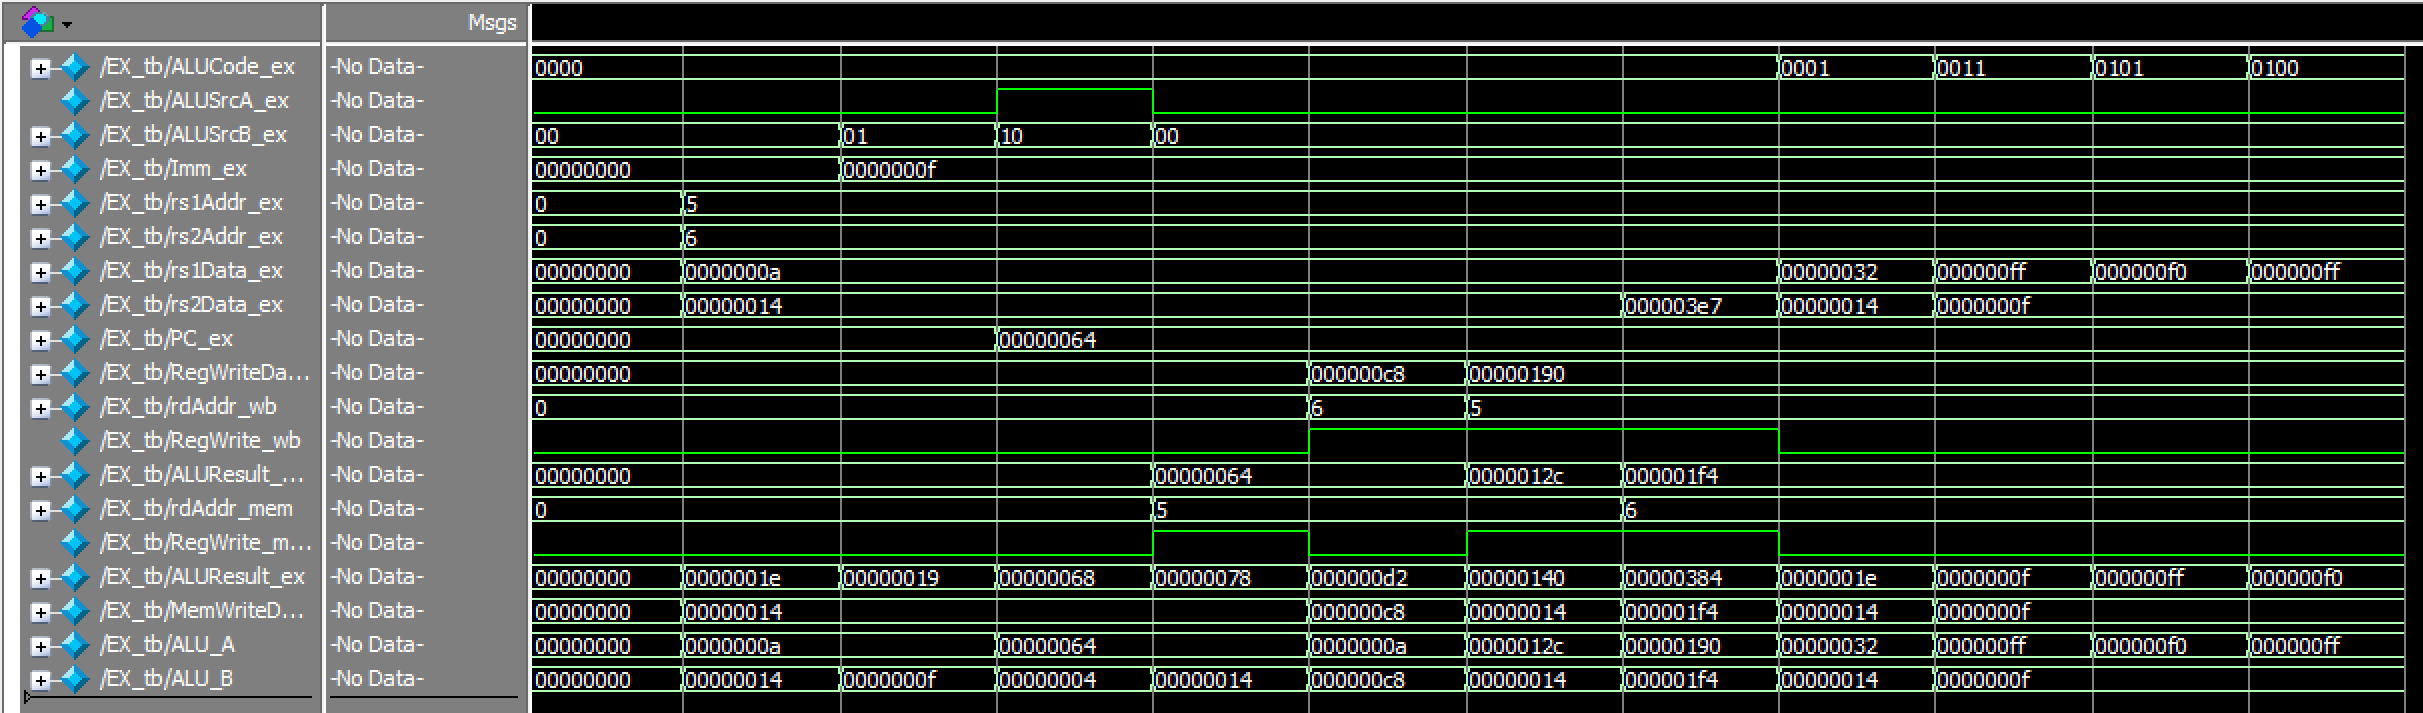
\includegraphics[width=1\textwidth]{EX.png}
    \caption{EX模块仿真波形}
\end{figure}

\subsubsection{实验结果分析}

通过 ModelSim 对 EX 模块进行功能仿真，重点测试数据前推机制、操作数选择逻辑和 ALU 运算功能的集成。测试用例及预期结果如下：

\textbf{Test 1: 简单加法（无前推）}

\begin{table}[H]
\centering
\begin{tabular}{|c|c|c|c|c|c|c|}
\hline
ALUCode & ALUSrcA & ALUSrcB & rs1Data & rs2Data & ALU\_A（预期） & ALU\_B（预期） \\ \hline
alu\_add & 0 & 2'b00 & 32'd10 & 32'd20 & 32'd10 & 32'd20 \\ \hline
\multicolumn{7}{|c|}{ALUResult（预期）：32'd30} \\ \hline
\end{tabular}
\caption{验证基本加法运算，无数据相关}
\end{table}

\textbf{Test 2: 加法与立即数}

\begin{table}[H]
\centering
\begin{tabular}{|c|c|c|c|c|c|c|}
\hline
ALUCode & ALUSrcA & ALUSrcB & rs1Data & Imm & ALU\_A（预期） & ALU\_B（预期） \\ \hline
alu\_add & 0 & 2'b01 & 32'd10 & 32'd15 & 32'd10 & 32'd15 \\ \hline
\multicolumn{7}{|c|}{ALUResult（预期）：32'd25} \\ \hline
\end{tabular}
\caption{验证 I-type 指令立即数操作}
\end{table}

\textbf{Test 3: PC + 4 运算}

\begin{table}[H]
\centering
\begin{tabular}{|c|c|c|c|c|c|}
\hline
ALUCode & ALUSrcA & ALUSrcB & PC & ALU\_A（预期） & ALU\_B（预期） \\ \hline
alu\_add & 1 & 2'b10 & 32'd100 & 32'd100 & 32'd4 \\ \hline
\multicolumn{6}{|c|}{ALUResult（预期）：32'd104} \\ \hline
\end{tabular}
\caption{验证 PC+4 计算（用于顺序执行）}
\end{table}

\textbf{Test 4: MEM 阶段前推到 rs1}

\begin{table}[H]
\centering
\begin{tabular}{|c|c|c|c|c|c|}
\hline
rs1Addr & rdAddr\_mem & ALUResult\_mem & RegWrite\_mem & rs1Data & ForwardA（预期） \\ \hline
5 & 5 & 32'd100 & 1 & 32'd10 & 2'b10 \\ \hline
\multicolumn{6}{|c|}{ALU\_A（预期）：32'd100（来自 MEM 前推），ALU\_B：32'd20，ALUResult：32'd120} \\ \hline
\end{tabular}
\caption{验证 EX-MEM 一阶数据相关的前推}
\end{table}

\textbf{Test 5: WB 阶段前推到 rs2}

\begin{table}[H]
\centering
\begin{tabular}{|c|c|c|c|c|c|}
\hline
rs2Addr & rdAddr\_wb & RegWriteData\_wb & RegWrite\_wb & rs2Data & ForwardB（预期） \\ \hline
6 & 6 & 32'd200 & 1 & 32'd20 & 2'b01 \\ \hline
\multicolumn{6}{|c|}{ALU\_A：32'd10，ALU\_B（预期）：32'd200（来自 WB 前推），ALUResult：32'd210} \\ \hline
\end{tabular}
\caption{验证 MEM-WB 二阶数据相关的前推}
\end{table}

\textbf{Test 6: MEM 前推优先级高于 WB}

\begin{table}[H]
\centering
\begin{tabular}{|c|c|c|c|c|c|}
\hline
rs1Addr & rdAddr\_mem & rdAddr\_wb & ALUResult\_mem & RegWriteData\_wb & ForwardA（预期） \\ \hline
5 & 5 & 5 & 32'd300 & 32'd400 & 2'b10 \\ \hline
\multicolumn{6}{|c|}{ALU\_A（预期）：32'd300（MEM 前推，忽略 WB），ALUResult：32'd320} \\ \hline
\end{tabular}
\caption{验证前推优先级：MEM > WB}
\end{table}

\textbf{Test 7: MemWriteData 前推（SW 指令）}

\begin{table}[H]
\centering
\begin{tabular}{|c|c|c|c|c|c|}
\hline
rs2Addr & rdAddr\_mem & ALUResult\_mem & RegWrite\_mem & rs2Data & ForwardB（预期） \\ \hline
6 & 6 & 32'd500 & 1 & 32'd999 & 2'b10 \\ \hline
\multicolumn{6}{|c|}{MemWriteData\_ex（预期）：32'd500（前推值，用于 SW 指令）} \\ \hline
\end{tabular}
\caption{验证存储器写数据的前推}
\end{table}

\textbf{Test 8: SUB 运算}

\begin{table}[H]
\centering
\begin{tabular}{|c|c|c|c|c|}
\hline
ALUCode & rs1Data & rs2Data & ALU\_A（预期） & ALU\_B（预期） \\ \hline
alu\_sub & 32'd50 & 32'd20 & 32'd50 & 32'd20 \\ \hline
\multicolumn{5}{|c|}{ALUResult（预期）：32'd30} \\ \hline
\end{tabular}
\caption{验证减法运算}
\end{table}

\textbf{Test 9: AND 运算}

\begin{table}[H]
\centering
\begin{tabular}{|c|c|c|c|}
\hline
ALUCode & rs1Data & rs2Data & ALUResult（预期） \\ \hline
alu\_and & 32'h000000FF & 32'h0000000F & 32'h0000000F \\ \hline
\end{tabular}
\caption{验证按位与运算}
\end{table}

\textbf{Test 10: OR 运算}

\begin{table}[H]
\centering
\begin{tabular}{|c|c|c|c|}
\hline
ALUCode & rs1Data & rs2Data & ALUResult（预期） \\ \hline
alu\_or & 32'h000000F0 & 32'h0000000F & 32'h000000FF \\ \hline
\end{tabular}
\caption{验证按位或运算}
\end{table}

\textbf{Test 11: XOR 运算}

\begin{table}[H]
\centering
\begin{tabular}{|c|c|c|c|}
\hline
ALUCode & rs1Data & rs2Data & ALUResult（预期） \\ \hline
alu\_xor & 32'h000000FF & 32'h0000000F & 32'h000000F0 \\ \hline
\end{tabular}
\caption{验证按位异或运算}
\end{table}

仿真结果验证了以下功能：
\begin{enumerate}
    \item \textbf{数据前推机制}：正确检测并解决 EX-MEM（一阶）和 MEM-WB（二阶）数据相关，MEM 前推优先级高于 WB。
    \item \textbf{操作数选择}：ALUSrcA 和 ALUSrcB 能正确选择 PC、rs1/rs2 数据、立即数或常数 4。
    \item \textbf{前推数据路径}：ForwardA 和 ForwardB 多路选择器正确选择寄存器堆数据或前推数据。
    \item \textbf{ALU 集成}：ALU 模块与前推逻辑无缝集成，所有算术逻辑运算结果正确。
    \item \textbf{存储器写数据}：MemWriteData\_ex 正确输出前推后的 rs2 数据，支持 SW 指令。
    \item \textbf{流水线优化}：数据前推机制避免了流水线停顿，提高了 CPU 执行效率。
\end{enumerate}

综合测试表明，EX 模块成功实现了执行阶段的全部功能，包括 ALU 运算、数据前推和操作数选择，为流水线 CPU 的高效运行提供了保障。

\clearpage
\subsection{IF模块设计}
\subsubsection{设计原理}

IF 模块由指令指针寄存器（PC）、指令存储器子模块（Instruction ROM）、指令指针选择器（MUX）和一个 32 位加法器组成。IF 模块接口信息如表 30.10 所示。

\begin{figure}[H]
    \centering
    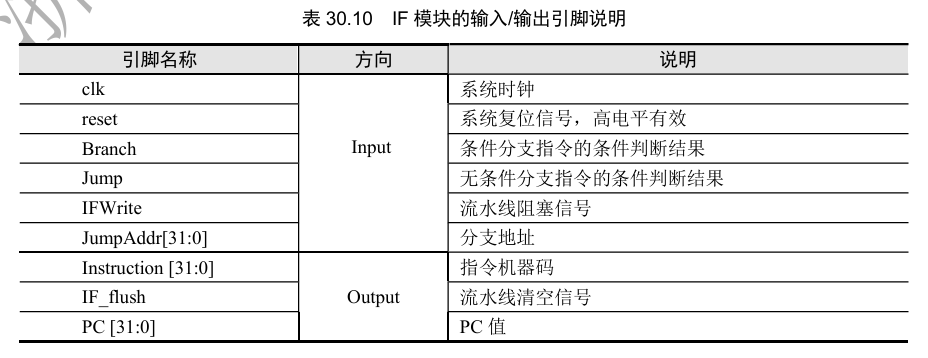
\includegraphics[width=0.9\textwidth]{e13.png}
    \caption{IF 模块的输入/输出引脚说明}
\end{figure}

由图 30.3 可看出，指令存储器为组合存储器，可用 Verilog HDL 设计一个查找表阵列 ROM。考虑到 FPGA 的资源，该 ROM 容量可设计为 $64\times32$bit。作者提供一个指令存储器模块 InstructionROM.v，ROM 内存放一段简单测试程序的机器码，对应的测试程序为：

\begin{lstlisting}[language=verilog]
lui  X30, 0x3000
jalr X31, later(X0)
earlier:sw  X28, 0x0C(X0)
lw  X29, 4(X6)
slliX5,  X29, 2              //数据冒险
lw  X28, 4(X6)
sltuX28,X6,X7
done:jal  X31, done
later: bneX0, X0, end         // 分支条件不成立
addi X5, X30, 0x42
add X6, X0, X31
sub X7,  X5, X6  //操作 A 二阶数据相关, 操作 B 一阶数据相关
or  X28, X7, X5   //操作 A 一阶数据相关, 操作 B 三阶数据相关
beq X0, X0, earlier  // 分支条件成立
end:  nop
\end{lstlisting}

\subsubsection{Verilog HDL代码与设计分析}

\textbf{(1) 模块接口定义}

IF 模块负责取指令操作，包含分支和跳转控制、流水线停顿控制以及流水线清空功能。

\begin{lstlisting}[language=verilog]
module IF1(clk, reset, Branch, Jump, IFWrite, JumpAddr, 
           Instruction_if, PC, IF_flush);
    input clk;
    input reset;
    input Branch;          // 分支指令的条件判断结果
    input Jump;            // 无条件分支指令的条件判断结果
    input IFWrite;         // 流水线阻塞暂停信号
    input [31:0] JumpAddr; // 分支地址
    output [31:0] Instruction_if;  // 指令机器码
    output [31:0] PC;               // PC 值
    output IF_flush;                // 流水线清空信号
\end{lstlisting}

\textbf{(2) 内部信号定义}

定义 PC 寄存器、PC+4 计算结果、下一条 PC 值选择信号等内部信号。

\begin{lstlisting}[language=verilog]
// Internal signals
reg [31:0] PC_reg;
wire [31:0] PC_plus_4;
wire co_unused;
wire PCSource;
wire [31:0] Next_PC;

assign PC = PC_reg;
\end{lstlisting}

\textbf{(3) PC+4 加法器}

使用 32 位加法器计算顺序执行时的下一条指令地址 PC+4。

\begin{lstlisting}[language=verilog]
// 32-bit adder: calculate PC + 4
adder_32bits u_adder_pc (
    .a(PC_reg),
    .b(32'd4),
    .ci(1'b0),
    .s(PC_plus_4),
    .co(co_unused)
);
\end{lstlisting}

\textbf{(4) PC 源选择逻辑}

根据 Branch 或 Jump 信号决定下一条 PC 是跳转地址还是 PC+4。当发生分支或跳转时，选择 JumpAddr；否则选择 PC+4 实现顺序执行。

\begin{lstlisting}[language=verilog]
// PCSource MUX: select next PC (Branch or Jump)
assign PCSource = Branch | Jump;
assign Next_PC = PCSource ? JumpAddr : PC_plus_4;
\end{lstlisting}

\textbf{(5) PC 寄存器与流水线停顿控制}

PC 寄存器在时钟上升沿更新。复位时 PC 清零，IFWrite 信号控制流水线停顿：当 IFWrite=0 时，PC 保持不变，实现流水线阻塞。

\begin{lstlisting}[language=verilog]
// PC register with enable (IFWrite) for pipeline stall
always @(posedge clk)
    if (reset)
        PC_reg <= 32'd0;
    else if (IFWrite)
        PC_reg <= Next_PC;
\end{lstlisting}

\textbf{(6) 指令存储器例化}

指令 ROM 容量为 64×32bit，使用 PC[7:2] 作为地址索引（因为指令按字对齐，低 2 位始终为 0）。

\begin{lstlisting}[language=verilog]
// Instruction ROM (64x32bit, address is PC[7:2])
InstructionROM u_InstructionROM (
    .addr(PC_reg[7:2]), 
    .dout(Instruction_if)
);
\end{lstlisting}

\textbf{(7) 流水线清空信号}

当发生分支或跳转时，IF\_flush 信号置 1，用于清空 IF/ID 流水线寄存器中的无效指令（分支延迟槽处理）。

\begin{lstlisting}[language=verilog]
// IF_flush signal to clear IF/ID register
assign IF_flush = PCSource;
\end{lstlisting}

\subsubsection{ModelSim仿真波形}
\begin{figure}[H]
    \centering
    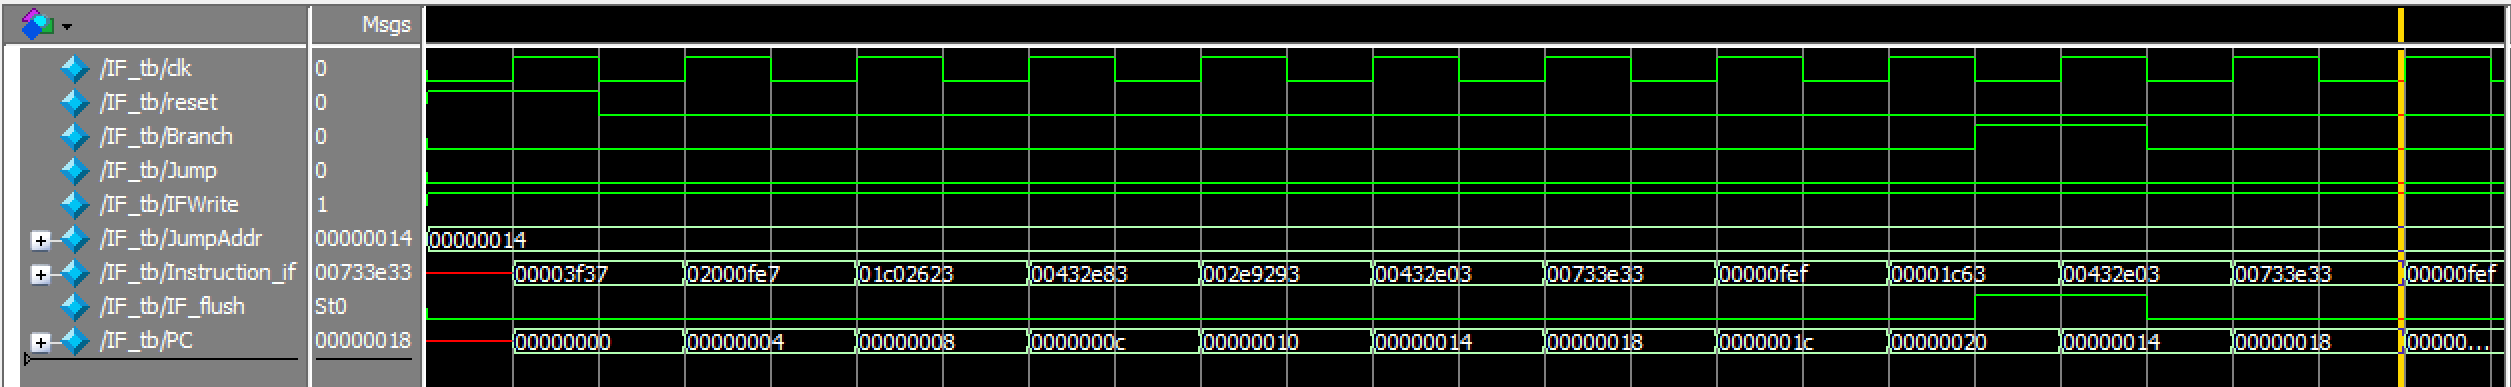
\includegraphics[width=1\textwidth]{IF1.png}
    \caption{IF模块仿真波形前半部分}
\end{figure}
\begin{figure}[H]
    \centering
    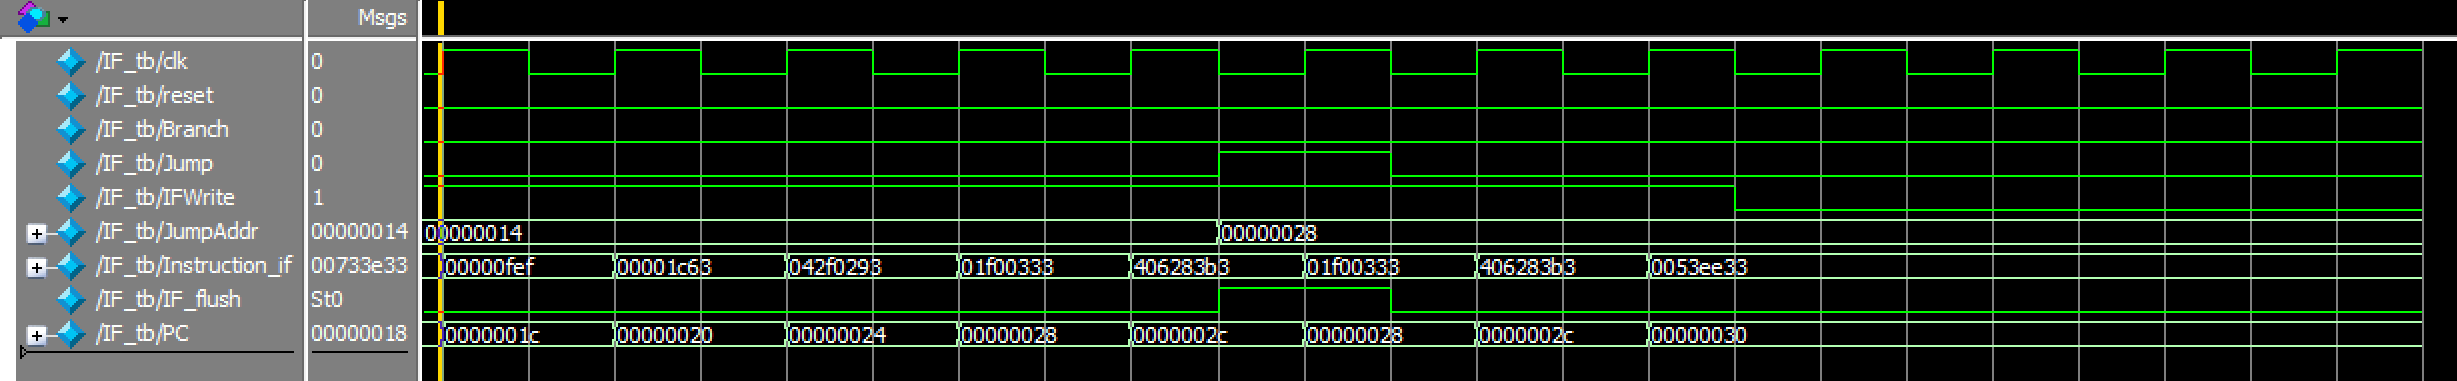
\includegraphics[width=1\textwidth]{IF2.png}
    \caption{IF模块仿真波形后半部分}
\end{figure}
\subsubsection{实验结果分析}

通过 ModelSim 对 IF 模块进行功能仿真，测试了正常取指、分支跳转、无条件跳转和流水线停顿等功能。测试用例及预期结果如下：

\textbf{Test 1: 复位与初始化}

\begin{table}[H]
\centering
\begin{tabular}{|c|c|c|c|c|}
\hline
时刻 & reset & Branch & Jump & PC（预期） \\ \hline
0-100ns & 1 & 0 & 0 & 32'd0 \\ \hline
\multicolumn{5}{|c|}{验证复位功能：PC 初始化为 0} \\ \hline
\end{tabular}
\caption{验证复位功能}
\end{table}

\textbf{Test 2: 顺序取指（PC+4）}

\begin{table}[H]
\centering
\begin{tabular}{|c|c|c|c|c|c|}
\hline
时刻 & IFWrite & Branch & Jump & PC（当前） & PC（下一周期预期） \\ \hline
100ns & 1 & 0 & 0 & 0 & 4 \\ \hline
150ns & 1 & 0 & 0 & 4 & 8 \\ \hline
200ns & 1 & 0 & 0 & 8 & 12 \\ \hline
250ns & 1 & 0 & 0 & 12 & 16 \\ \hline
\multicolumn{6}{|c|}{验证顺序执行：每个时钟周期 PC 递增 4} \\ \hline
\end{tabular}
\caption{验证顺序取指功能}
\end{table}

\textbf{Test 3: 分支跳转（Branch）}

\begin{table}[H]
\centering
\begin{tabular}{|c|c|c|c|c|c|}
\hline
时刻 & Branch & Jump & JumpAddr & PCSource（预期） & IF\_flush（预期） \\ \hline
800ns & 1 & 0 & 32'd20 & 1 & 1 \\ \hline
\multicolumn{6}{|c|}{下一时钟周期 PC（预期）：32'd20（跳转到分支目标地址）} \\ \hline
\end{tabular}
\caption{验证条件分支跳转}
\end{table}

\textbf{Test 4: 分支后恢复顺序执行}

\begin{table}[H]
\centering
\begin{tabular}{|c|c|c|c|c|}
\hline
时刻 & Branch & Jump & PC（当前） & PC（下一周期预期） \\ \hline
900ns & 0 & 0 & 20 & 24 \\ \hline
950ns & 0 & 0 & 24 & 28 \\ \hline
1000ns & 0 & 0 & 28 & 32 \\ \hline
\multicolumn{5}{|c|}{验证分支后恢复顺序执行：PC 继续递增} \\ \hline
\end{tabular}
\caption{验证分支后顺序执行}
\end{table}

\textbf{Test 5: 无条件跳转（Jump）}

\begin{table}[H]
\centering
\begin{tabular}{|c|c|c|c|c|c|}
\hline
时刻 & Branch & Jump & JumpAddr & PCSource（预期） & IF\_flush（预期） \\ \hline
1500ns & 0 & 1 & 32'd40 & 1 & 1 \\ \hline
\multicolumn{6}{|c|}{下一时钟周期 PC（预期）：32'd40（跳转到目标地址）} \\ \hline
\end{tabular}
\caption{验证无条件跳转（jal/jalr）}
\end{table}

\textbf{Test 6: 跳转后恢复顺序执行}

\begin{table}[H]
\centering
\begin{tabular}{|c|c|c|c|c|}
\hline
时刻 & Branch & Jump & PC（当前） & PC（下一周期预期） \\ \hline
1600ns & 0 & 0 & 40 & 44 \\ \hline
1650ns & 0 & 0 & 44 & 48 \\ \hline
\multicolumn{5}{|c|}{验证跳转后恢复顺序执行} \\ \hline
\end{tabular}
\caption{验证跳转后顺序执行}
\end{table}

\textbf{Test 7: 流水线停顿（IFWrite=0）}

\begin{table}[H]
\centering
\begin{tabular}{|c|c|c|c|c|}
\hline
时刻 & IFWrite & PC（当前） & PC（下一周期预期） & 说明 \\ \hline
1700ns & 0 & 48 & 48（保持） & 流水线停顿开始 \\ \hline
1750ns & 0 & 48 & 48（保持） & PC 保持不变 \\ \hline
1800ns & 0 & 48 & 48（保持） & PC 继续保持 \\ \hline
1850ns & 0 & 48 & 48（保持） & PC 继续保持 \\ \hline
\multicolumn{5}{|c|}{验证流水线停顿：IFWrite=0 时 PC 保持不变，实现阻塞} \\ \hline
\end{tabular}
\caption{验证流水线停顿功能}
\end{table}

\textbf{Test 8: 指令读取验证}

\begin{table}[H]
\centering
\begin{tabular}{|c|c|c|}
\hline
PC 值 & ROM 地址 & Instruction\_if（预期） \\ \hline
0 & PC[7:2]=0 & ROM[0] 的指令 \\ \hline
4 & PC[7:2]=1 & ROM[1] 的指令 \\ \hline
8 & PC[7:2]=2 & ROM[2] 的指令 \\ \hline
20 & PC[7:2]=5 & ROM[5] 的指令 \\ \hline
40 & PC[7:2]=10 & ROM[10] 的指令 \\ \hline
\multicolumn{3}{|c|}{验证指令存储器正确读取：地址使用 PC[7:2] 索引} \\ \hline
\end{tabular}
\caption{验证指令读取功能}
\end{table}

仿真结果验证了以下功能：
\begin{enumerate}
    \item \textbf{复位功能}：reset 信号有效时，PC 正确初始化为 0。
    \item \textbf{顺序取指}：正常情况下，PC 每个时钟周期递增 4，实现顺序执行。
    \item \textbf{分支跳转}：Branch 信号有效时，PC 跳转到 JumpAddr 指定的分支目标地址。
    \item \textbf{无条件跳转}：Jump 信号有效时，PC 跳转到 JumpAddr 指定的跳转目标地址。
    \item \textbf{流水线清空}：PCSource（Branch|Jump）信号生成 IF\_flush，用于清空 IF/ID 寄存器。
    \item \textbf{流水线停顿}：IFWrite=0 时，PC 保持不变，实现流水线阻塞功能（用于解决 load-use 冒险）。
    \item \textbf{指令存储器}：正确使用 PC[7:2] 作为 ROM 地址索引，读取对应的指令机器码。
    \item \textbf{PC 源选择}：PCSource 多路选择器正确选择 PC+4 或 JumpAddr 作为下一条 PC 值。
\end{enumerate}

综合测试表明，IF 模块成功实现了取指阶段的全部功能，包括顺序取指、分支跳转控制、流水线停顿和清空机制，为流水线 CPU 的正确运行奠定了基础。

\clearpage
\subsection{MEM模块设计}
\subsubsection{设计原理}

MEM 模块包括数据存储器子模块（Data RAM）和一些外围信号与选择电路。

{\heiti DataRAM IP 内核生成}

{\heiti IP 内核生成步骤：}

在图所示的 Vivado 工程界面中，在 Flow Navigator 窗口下，点击 PROJECT MANAGER $\Rightarrow$ IP Catalog 命令；
然后在 Text Editor 窗口的 IP Catalog 选项卡中，找到并依次展开 Memories \& Storage Elements、RAMs \& ROMs；双击 RAMs \& ROMs 下面的 Distributed Memory Generator 选项，将会弹出后续所示的存储器 IP 内核产生向导。

\begin{figure}[H]
    \centering
    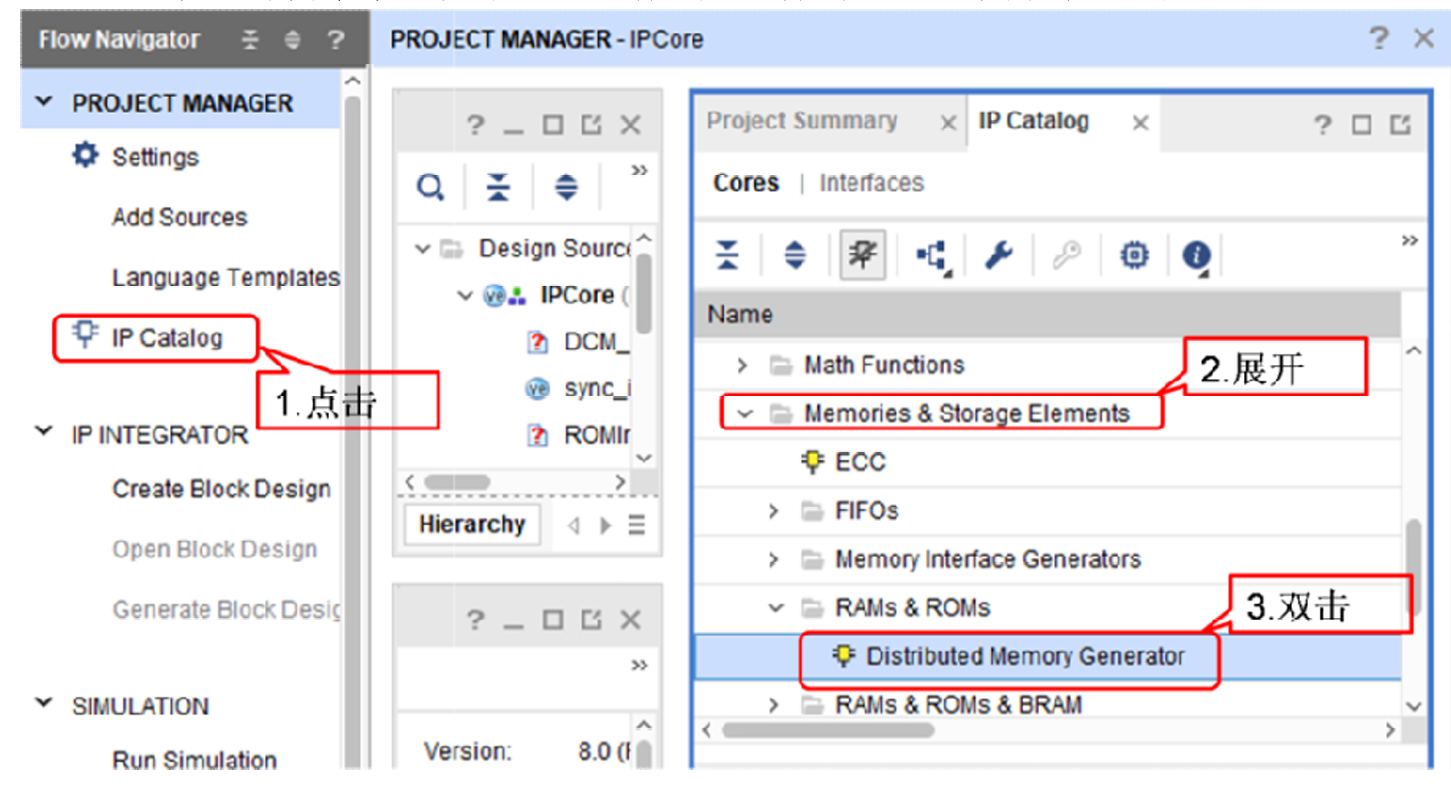
\includegraphics[width=0.95\textwidth]{e14.png}
    \caption{IP 选择对话框}
\end{figure}

{\heiti IP 内核配置：}

数据存储器可用 Xilinx 的 IP 内核实现。考虑到 FPGA 的资源，数据存储器可设计为容量为 $64\times32$ bit 的单端口 RAM，输出采用组合输出（Non Registered）。

如图，直接在 vivado 工程中，通过 IP Catalog，选择 RAM，并设置参数，生成 IP 内核。参数选择 32 位宽，64 个存储单元，single port RAM，non registered 输出。

之后，直接在 CPU 顶层模块中实例化数据存储器模块即可。

\begin{figure}[H]
    \centering
    \begin{minipage}[b]{0.45\linewidth}
        \centering
        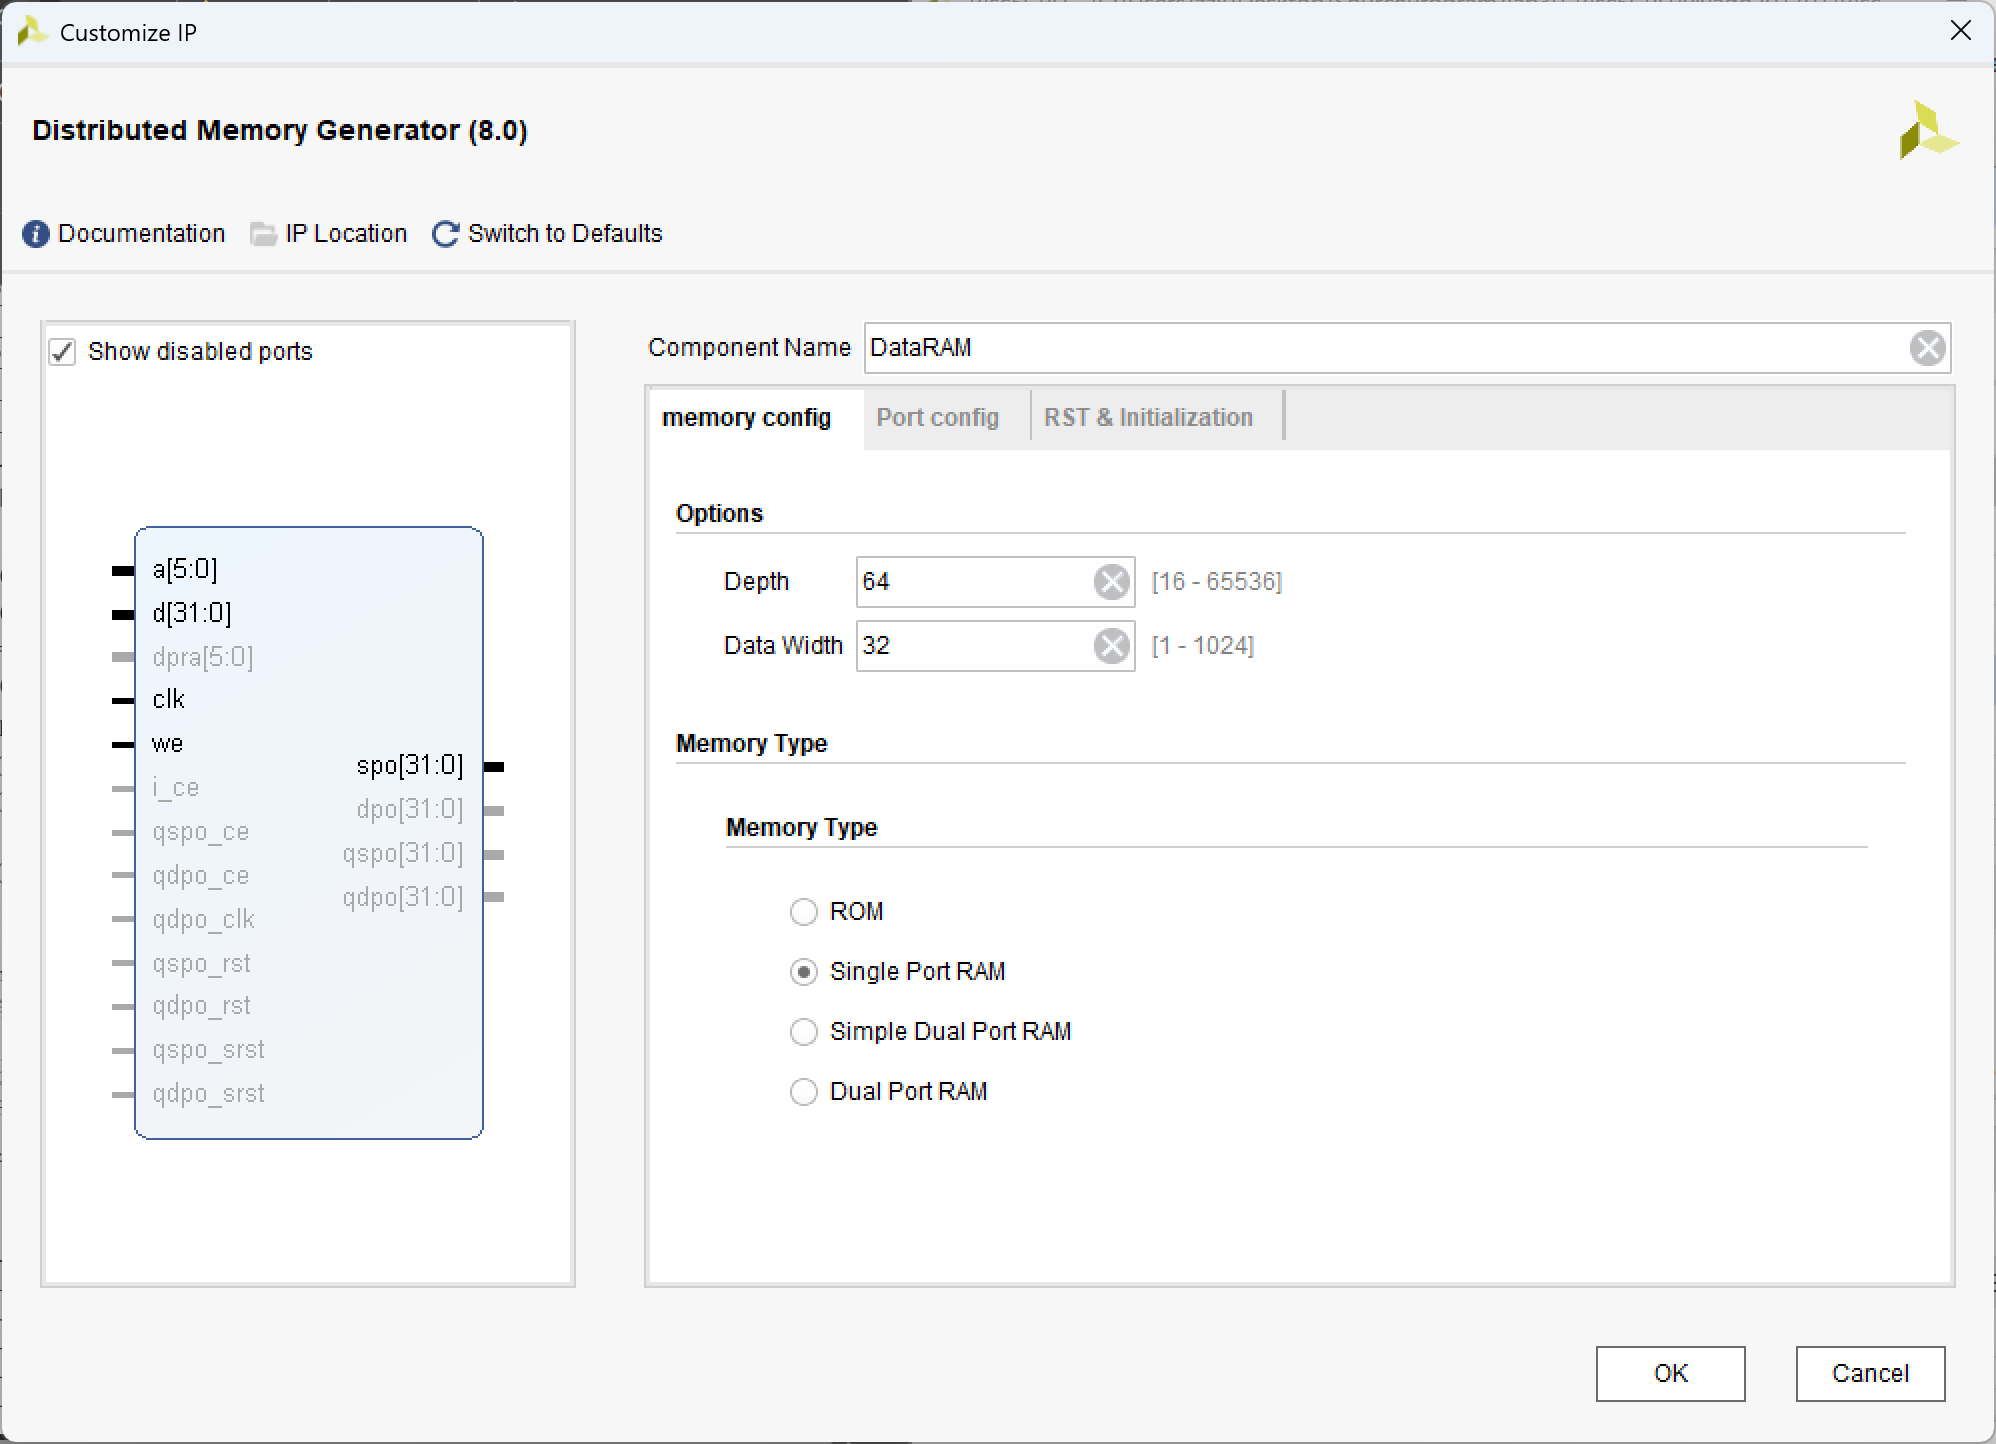
\includegraphics[width=0.9\textwidth]{p2.png}
        \caption{IP内核基本配置}
            
    \end{minipage}%
    \begin{minipage}[b]{0.45\linewidth}
        \centering
        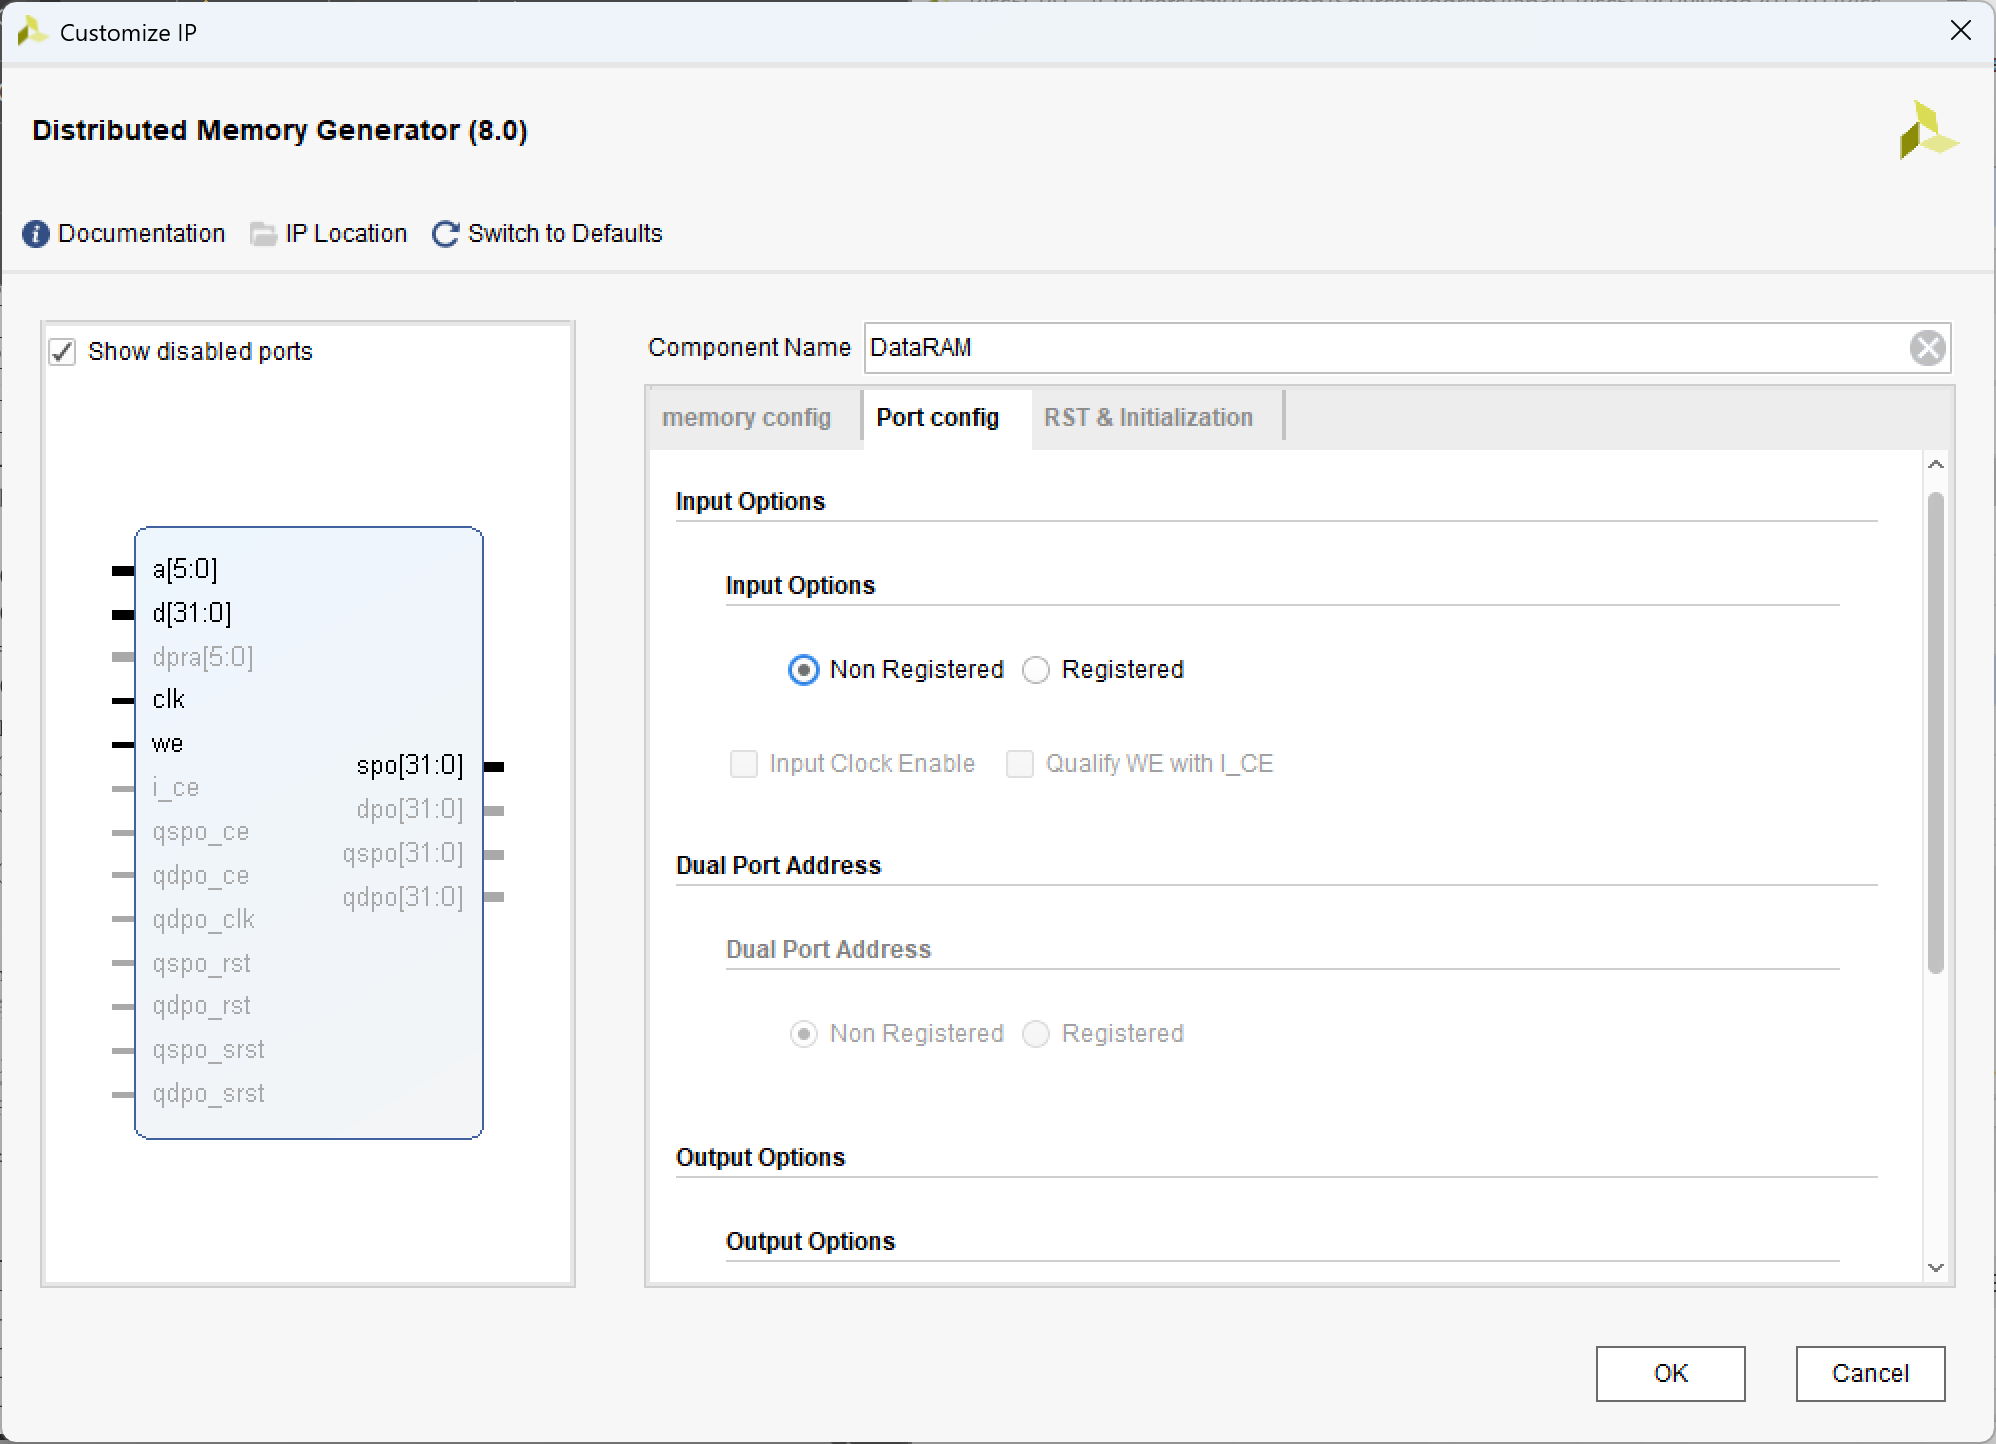
\includegraphics[width=0.9\textwidth]{p3.png}
        \caption{IP内核端口配置}
            
    \end{minipage}
\end{figure}

{\heiti MEM 模块设计}

MEM 模块较为简单，直接参考原理图，最后在 CPU 顶层模块中实现即可。

\clearpage
\subsection{CPU顶层设计}
\subsubsection{设计原理}

按照Figure 20所示的原理框图连接各模块即可。为了测试方便，可将关键变量输出，关键变量有：指令指针 PC、指令码 Instruction\_id、流水线插入气泡标志 Stall、分支标志 JumpFlag 即\{Jump, Branch\}、ALU 输入输出（ALU\_A、ALU\_B、ALUResult\_ex）和数据存储器的输出 MemDout\_mem。

\begin{figure}[H]
    \centering
    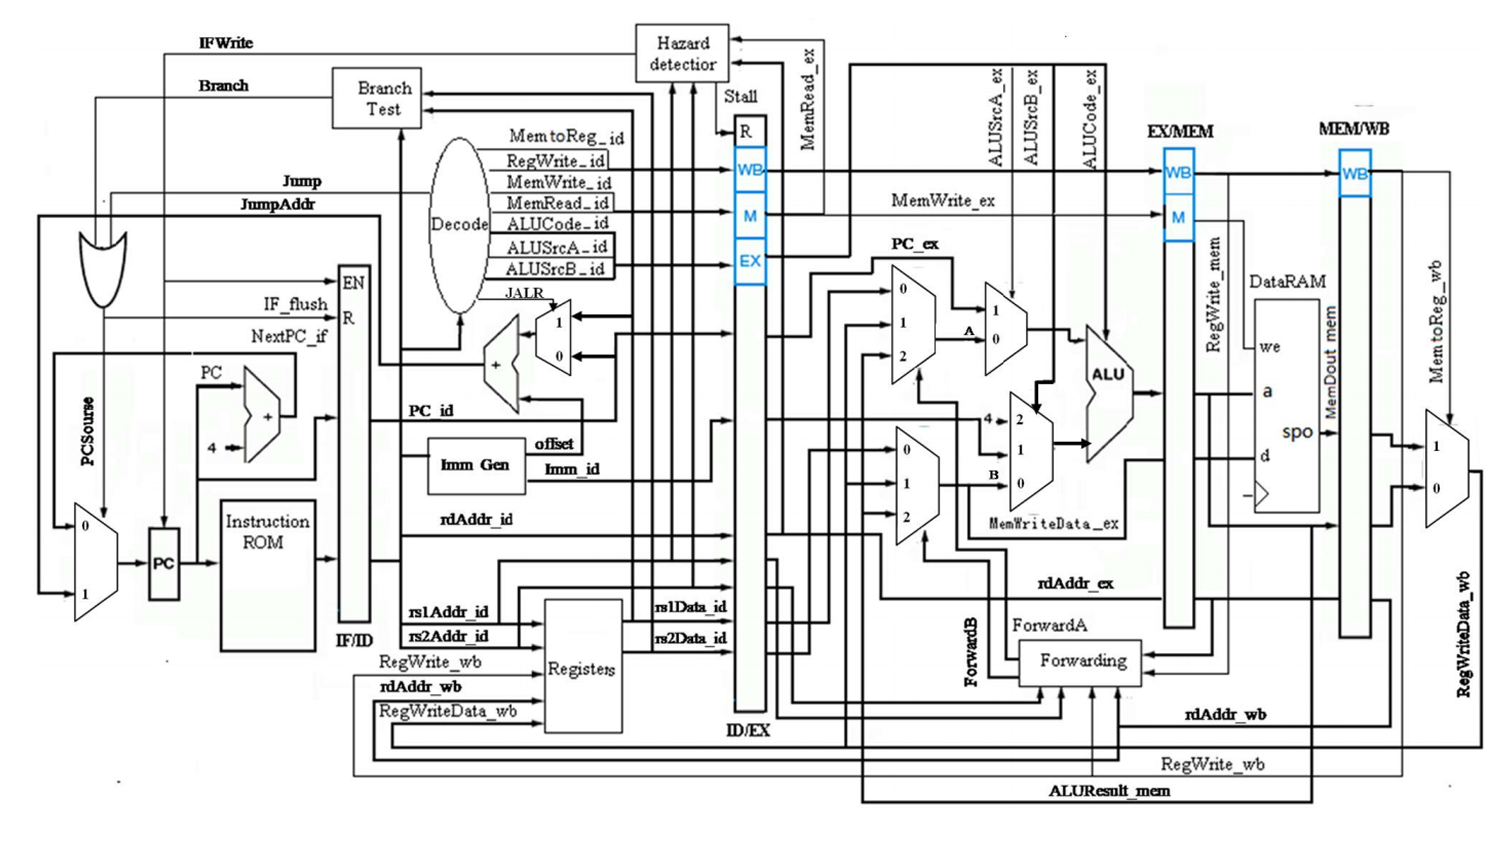
\includegraphics[width=0.9\textwidth]{e15.png}
    \caption{CPU 顶层模块的硬件连接图}
\end{figure}

\subsubsection{Verilog HDL代码与设计分析}

\textbf{(1) 流水线寄存器模块（DFF）}

为了规范流水线寄存器的设计，首先实现一个通用的 D 触发器模块，支持同步复位、清空和使能控制。

\begin{lstlisting}[language=verilog]
module DFF #(
    parameter WIDTH = 32
) (
    input clk,
    input reset,
    input clear,  // Sync clear (Stall/Flush)
    input en,     // Enable
    input [WIDTH-1:0] d,
    output reg [WIDTH-1:0] q
);
    always @(posedge clk)
        if (reset)
            q <= {WIDTH{1'b0}};
        else if (clear)
            q <= {WIDTH{1'b0}};
        else if (en)
            q <= d;
endmodule
\end{lstlisting}

该模块采用参数化设计，WIDTH 参数可配置寄存器位宽。优先级为：reset > clear > en，其中 clear 信号用于流水线清空（插入气泡），en 信号用于流水线停顿控制。

\textbf{(2) CPU 顶层模块接口}

CPU 顶层模块集成了五级流水线的所有阶段，并输出关键调试信号。

\begin{lstlisting}[language=verilog]
module Risc5CPU(
    input clk,
    input reset,
    output [1:0]  JumpFlag,        // {Jump, Branch}
    output [31:0] Instruction_id,  // 当前指令
    output [31:0] ALU_A,           // ALU 输入 A
    output [31:0] ALU_B,           // ALU 输入 B
    output [31:0] ALUResult_ex,    // ALU 结果
    output [31:0] PC,              // 程序计数器
    output [31:0] MemDout_mem,     // 存储器输出
    output        Stall            // 流水线停顿信号
);
\end{lstlisting}

\textbf{(3) 内部信号定义}

定义各流水线阶段之间的连接信号，包括控制信号和数据通路信号。

\begin{lstlisting}[language=verilog]
// IF Stage
wire [31:0] w_Instruction_if;
wire        w_IF_flush;

// ID Stage Control
wire        w_IFWrite;
wire [31:0] w_JumpAddr;
wire        w_Branch;
wire        w_Jump;

// ID Stage Outputs
wire        w_MemtoReg_id;
wire        w_RegWrite_id;
wire        w_MemWrite_id;
wire        w_MemRead_id;
wire [3:0]  w_ALUCode_id;
wire        w_ALUSrcA_id;
wire [1:0]  w_ALUSrcB_id;
wire [31:0] w_Imm_id;
wire [31:0] w_rs1Data_id;
wire [31:0] w_rs2Data_id;
wire [4:0]  w_rs1Addr_id;
wire [4:0]  w_rs2Addr_id;
wire [4:0]  w_rdAddr_id;

// EX Stage
wire [31:0] w_MemWriteData_ex;
wire [31:0] w_ALUResult_ex_internal;

// MEM Stage
wire [31:0] w_MemDout_mem_internal;

// WB Stage
wire [31:0] w_RegWriteData_wb;

// Pipeline Registers: IF/ID
// ... 省略
// Pipeline Registers: ID/EX
// ... 省略
// Pipeline Registers: EX/MEM
// ... 省略
// Pipeline Registers: MEM/WB 
// ... 省略
\end{lstlisting}

\textbf{(4) IF 阶段与 IF/ID 流水线寄存器}

IF 阶段负责取指令，IF/ID 寄存器存储 PC 和指令。

\begin{lstlisting}[language=verilog]
// Stage 1: IF (Instruction Fetch)
IF1 u_IF1 (
    ... // IF模块调用：PC输出
);

// Pipeline Register: IF/ID (64 bits: PC + Instruction)
DFF #(.WIDTH(64)) u_reg_IF_ID (
    .clk(clk),
    .reset(reset),
    .clear(w_IF_flush),      // 分支/跳转时清空
    .en(w_IFWrite),          // 停顿时禁止更新
    .d({PC, w_Instruction_if}),
    .q({r_PC_id, r_Instruction_id})
);
\end{lstlisting}

\textbf{(5) ID 阶段与 ID/EX 流水线寄存器}

ID 阶段进行指令译码、寄存器读取、冒险检测和分支判断。

\begin{lstlisting}[language=verilog]
// Stage 2: ID (Instruction Decode)
ID u_ID (
    ... // ID模块调用：指令译码、寄存器读取、冒险检测、分支判断等
);

// Pipeline Register: ID/EX (154 bits)
DFF #(.WIDTH(154)) u_reg_ID_EX (
    .clk(clk),
    .reset(reset),
    .clear(Stall),           // Stall 时插入气泡
    .en(1'b1),
    .d({w_MemtoReg_id, w_RegWrite_id, w_MemWrite_id, w_MemRead_id,
        w_ALUCode_id, w_ALUSrcA_id, w_ALUSrcB_id,
        w_Imm_id, w_rs1Data_id, w_rs2Data_id,
        w_rs1Addr_id, w_rs2Addr_id, w_rdAddr_id, r_PC_id}),
    .q({r_MemtoReg_ex, r_RegWrite_ex, r_MemWrite_ex, r_MemRead_ex,
        r_ALUCode_ex, r_ALUSrcA_ex, r_ALUSrcB_ex,
        r_Imm_ex, r_rs1Data_ex, r_rs2Data_ex,
        r_rs1Addr_ex, r_rs2Addr_ex, r_rdAddr_ex, r_PC_ex})
);
\end{lstlisting}

\textbf{(6) EX 阶段与 EX/MEM 流水线寄存器}

EX 阶段执行 ALU 运算和数据前推。

\begin{lstlisting}[language=verilog]
// Stage 3: EX (Execute)
EX u_EX (
    ... // EX模块调用：ALU运算、数据前推、操作数选择等
);

// Pipeline Register: EX/MEM (72 bits)
DFF #(.WIDTH(72)) u_reg_EX_MEM (
    .clk(clk),
    .reset(reset),
    .clear(1'b0),            // 正常流动，无需清空
    .en(1'b1),
    .d({w_ALUResult_ex_internal, w_MemWriteData_ex,
        r_MemWrite_ex, r_RegWrite_ex, r_MemtoReg_ex, r_rdAddr_ex}),
    .q({r_ALUResult_mem, r_MemWriteData_mem,
        r_MemWrite_mem, r_RegWrite_mem, r_MemtoReg_mem, r_rdAddr_mem})
);
\end{lstlisting}

\textbf{(7) MEM 阶段与 MEM/WB 流水线寄存器}

MEM 阶段访问数据存储器。

\begin{lstlisting}[language=verilog]
// Stage 4: MEM (Memory Access)
DataRAM u_DataRAM (
    ... // DataRAM模块调用：数据存储器读写操作
);

// Pipeline Register: MEM/WB (71 bits)
DFF #(.WIDTH(71)) u_reg_MEM_WB (
    .clk(clk),
    .reset(reset),
    .clear(1'b0),
    .en(1'b1),
    .d({w_MemDout_mem_internal, r_ALUResult_mem,
        r_RegWrite_mem, r_MemtoReg_mem, r_rdAddr_mem}),
    .q({r_MemDout_wb, r_ALUResult_wb,
        r_RegWrite_wb, r_MemtoReg_wb, r_rdAddr_wb})
);
\end{lstlisting}

\textbf{(8) WB 阶段与顶层输出}

WB 阶段选择写回寄存器堆的数据，并分配顶层输出信号。

\begin{lstlisting}[language=verilog]
// Stage 5: WB (Write Back)
assign w_RegWriteData_wb = r_MemtoReg_wb ? r_MemDout_wb : r_ALUResult_wb;

// Top-Level Output Assignments
assign JumpFlag       = {w_Jump, w_Branch};
assign Instruction_id = r_Instruction_id;
assign ALUResult_ex   = w_ALUResult_ex_internal;
assign MemDout_mem    = w_MemDout_mem_internal;
\end{lstlisting}

\textbf{设计要点分析：}

\begin{enumerate}
    \item \textbf{模块化流水线寄存器}：使用统一的 DFF 模块实现所有流水线寄存器，提高代码复用性和可维护性。
    \item \textbf{参数化设计}：DFF 模块的 WIDTH 参数根据各阶段数据位宽灵活配置（IF/ID: 64 位，ID/EX: 154 位，EX/MEM: 72 位，MEM/WB: 71 位）。
    \item \textbf{流水线控制}：IF/ID 寄存器受 IFWrite 和 IF\_flush 控制，ID/EX 寄存器受 Stall 控制，实现流水线停顿和清空。
    \item \textbf{调试信号输出}：顶层输出关键信号（PC、指令、ALU 输入输出、存储器输出、停顿标志）便于仿真调试。
    \item \textbf{层次化结构}：各流水线阶段独立封装为子模块（IF1、ID、EX），顶层仅负责模块例化和信号连接。
\end{enumerate}

\clearpage
\subsubsection{Vivado行为级仿真波形}
\begin{figure}[H]
    \centering
    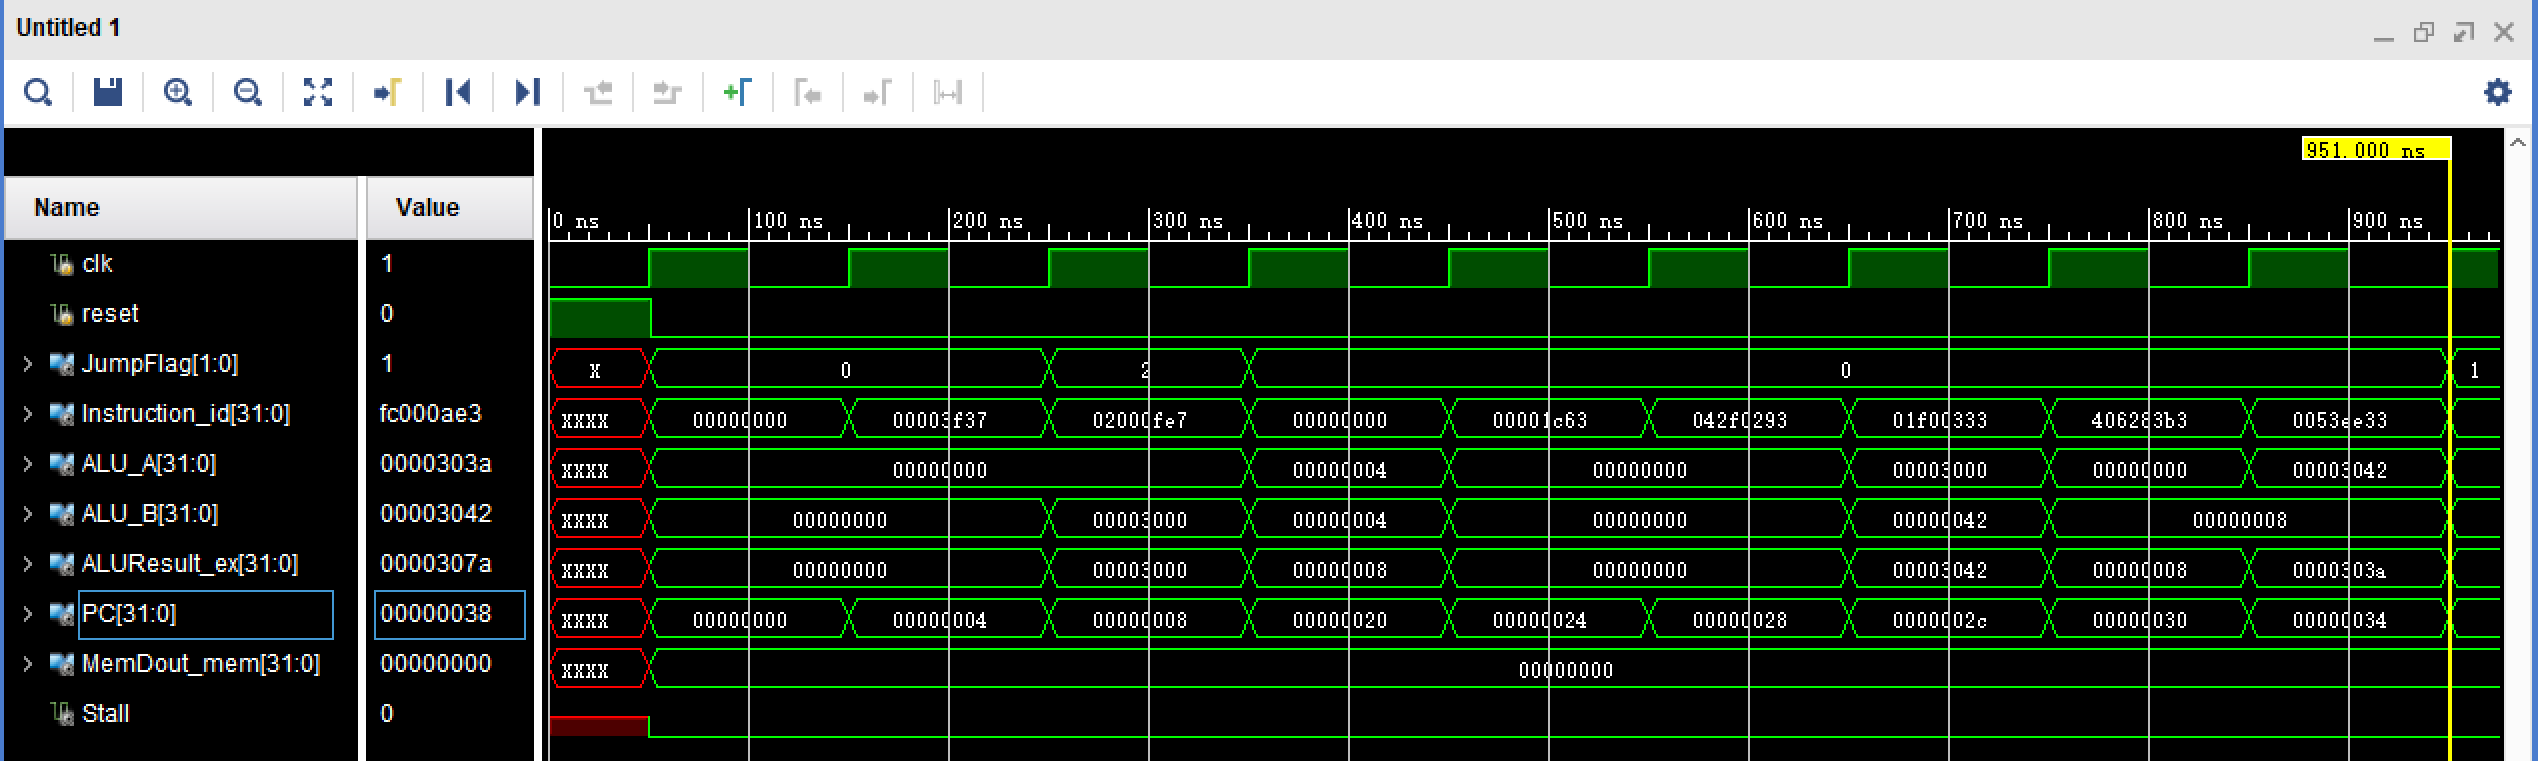
\includegraphics[width=1\textwidth]{CPU1.png}
    \caption{CPU总体仿真波形1}
\end{figure}
\begin{figure}[H]
    \centering
    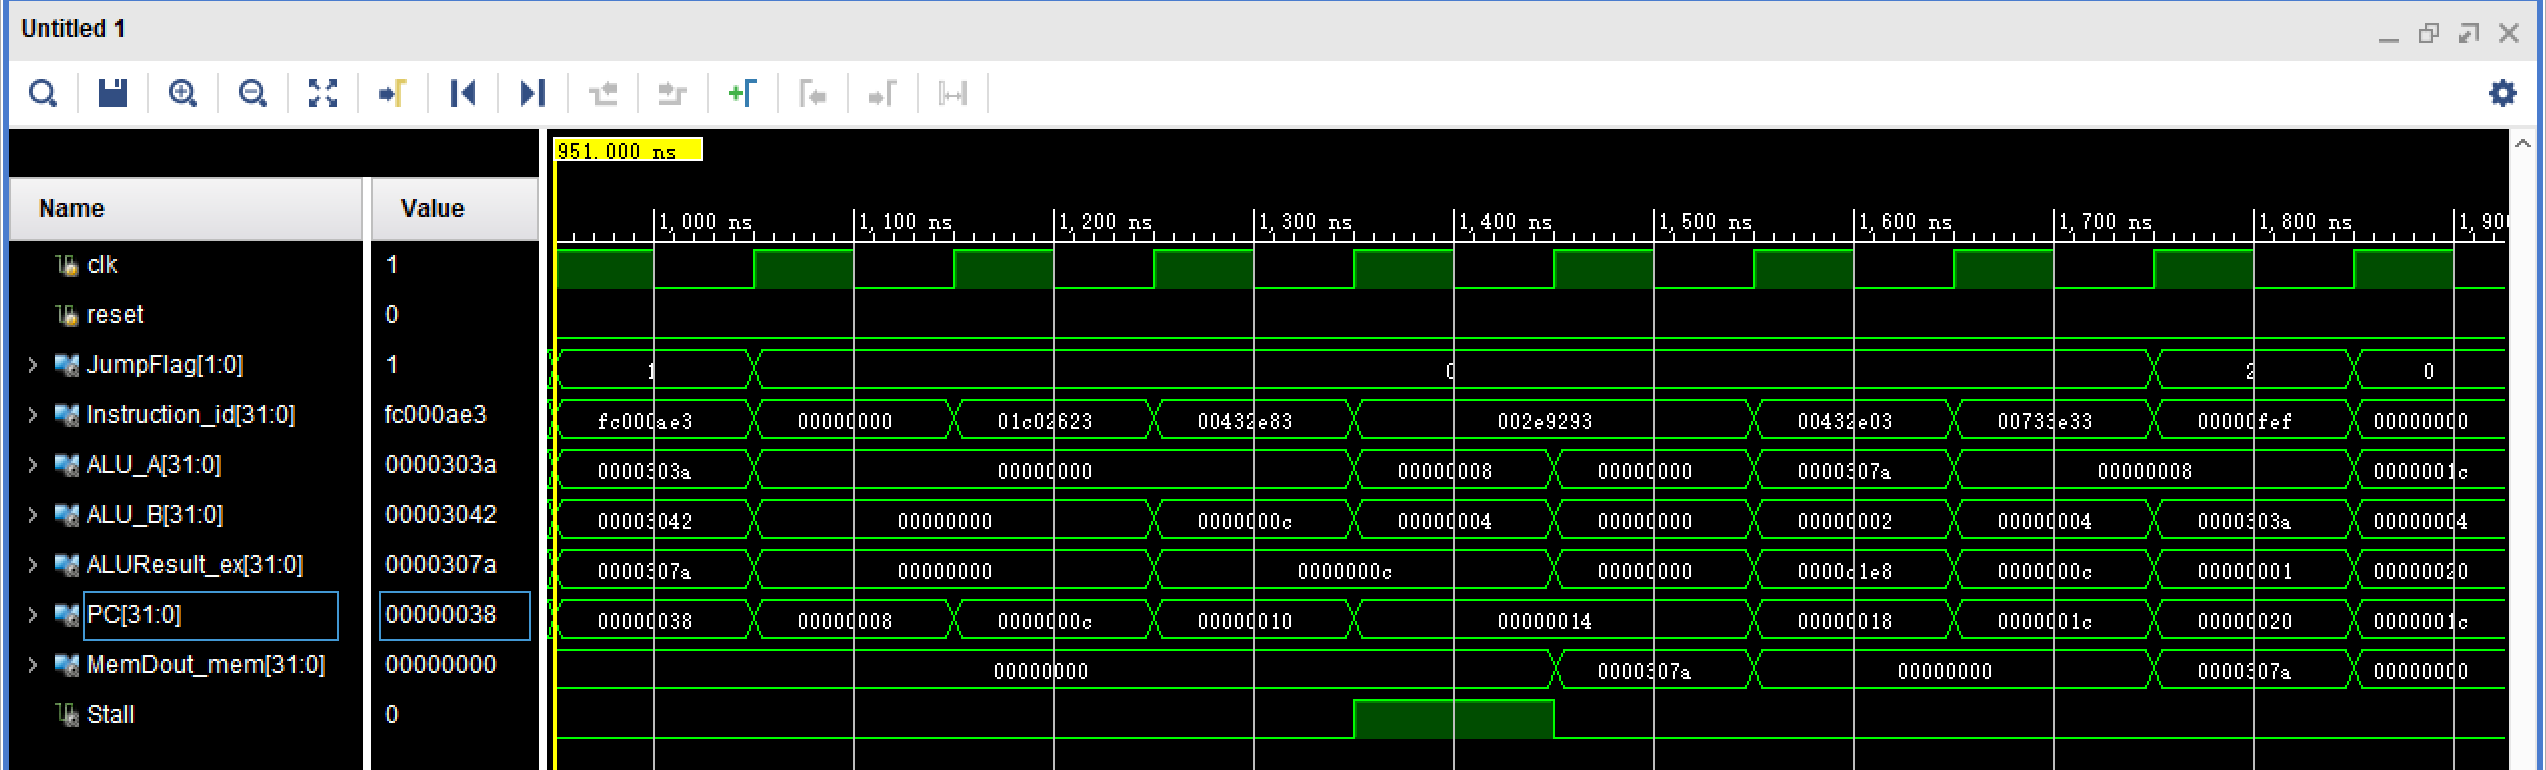
\includegraphics[width=1\textwidth]{CPU2.png}
    \caption{CPU总体仿真波形2}
\end{figure}\begin{figure}[H]
    \centering
    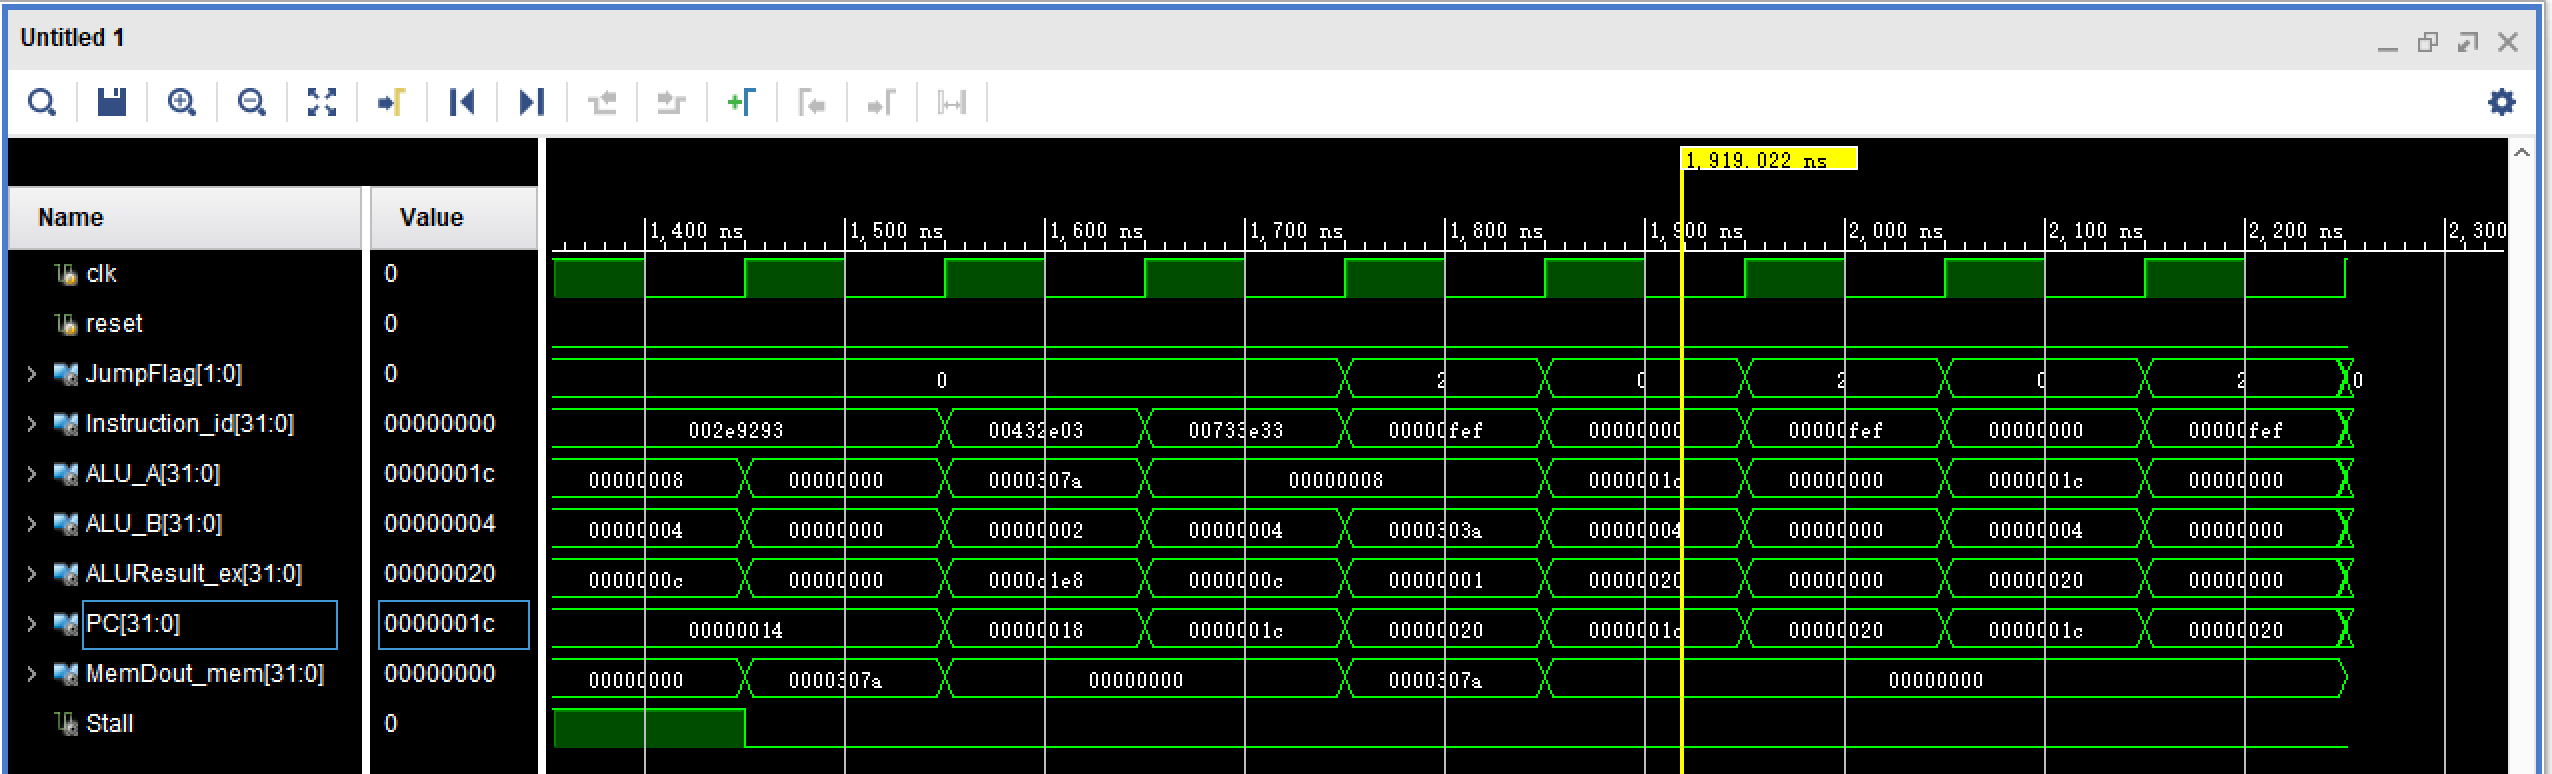
\includegraphics[width=1\textwidth]{CPU3.png}
    \caption{CPU总体仿真波形3}
\end{figure}
\subsubsection{实验结果分析}

与下图CPU总体仿真结果对照表对照，CPU顶层模块成功实现了五级流水线的各项功能。

\begin{figure}[H]
    \centering
    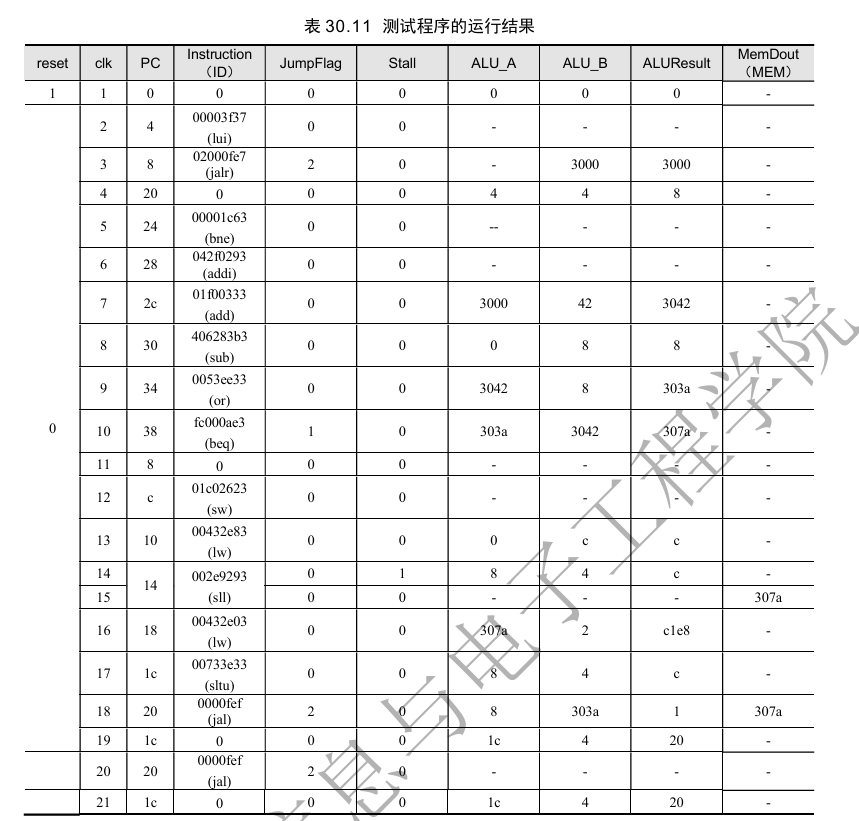
\includegraphics[width=1\textwidth]{e2.png}
    \caption{CPU总体仿真结果对照表}
\end{figure}

\clearpage
\section{实验结果}
再次打开Vivado 文件夹下的Risc5CPU.xpr 工程，添加流水线CPU设计的全部代
码，然后综合、实现和下载至NexysVideo 开发板。
连接带有HDMI接口的显示器，进行测试。首先将SW0置于低电平，使RISC-V
 CPU 工作在“单步”运行模式。复位后，每按一下上边按键，RISC-V CPU运行一步，
记录下显示器上的结果，对照CPU行为级仿真预期结果验证设计是否正确。下图截取了部分HDMI显示屏内容，经对照，结果均符合预期，设计正确。

注意：一般设计都采用同步复位，因此在"单步"运行模式时，如需要复位 CPU，应先按住"复位"按键（中间按键），再按上边按键才能复位。

\begin{figure}[H]
    \centering
    \subcaptionbox{HDMI显示屏显示内容1}[0.4\textwidth][c]{
        \centering
        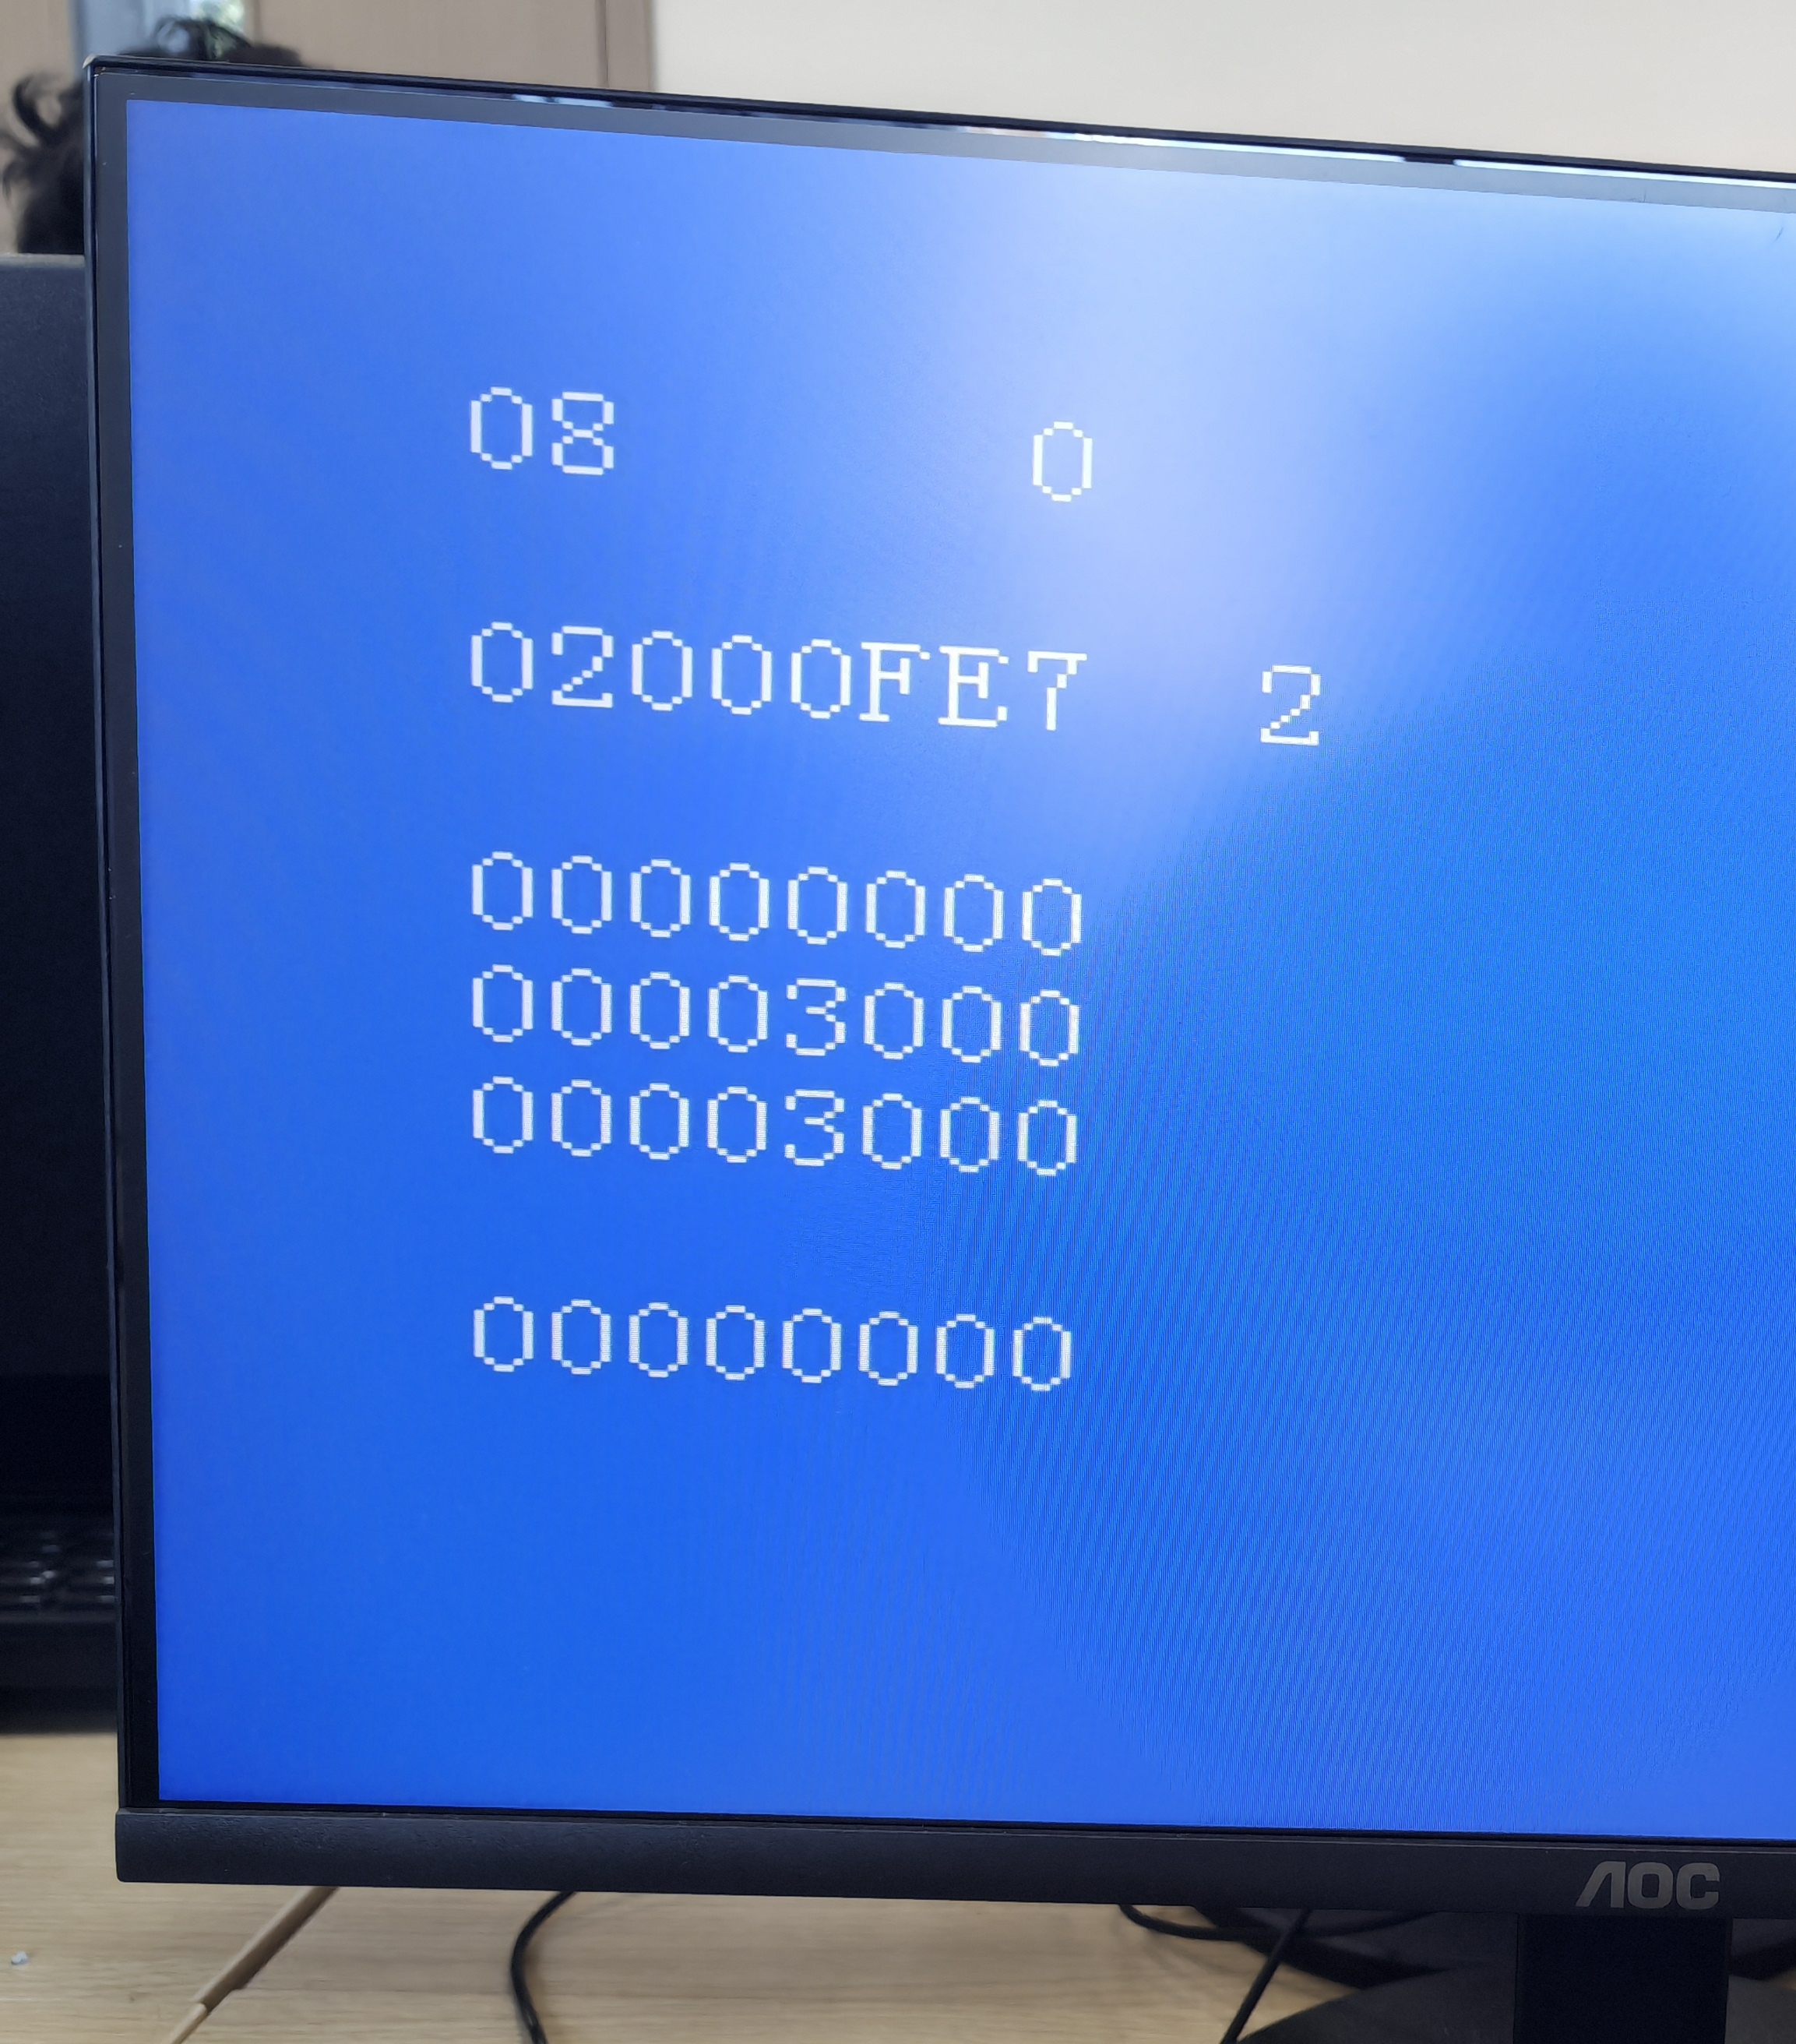
\includegraphics[width=0.4\textwidth]{r1.jpg}
    }%
    \hspace*{0.1cm}
    \subcaptionbox{HDMI显示屏显示内容2}[0.4\textwidth][c]{
        \centering
        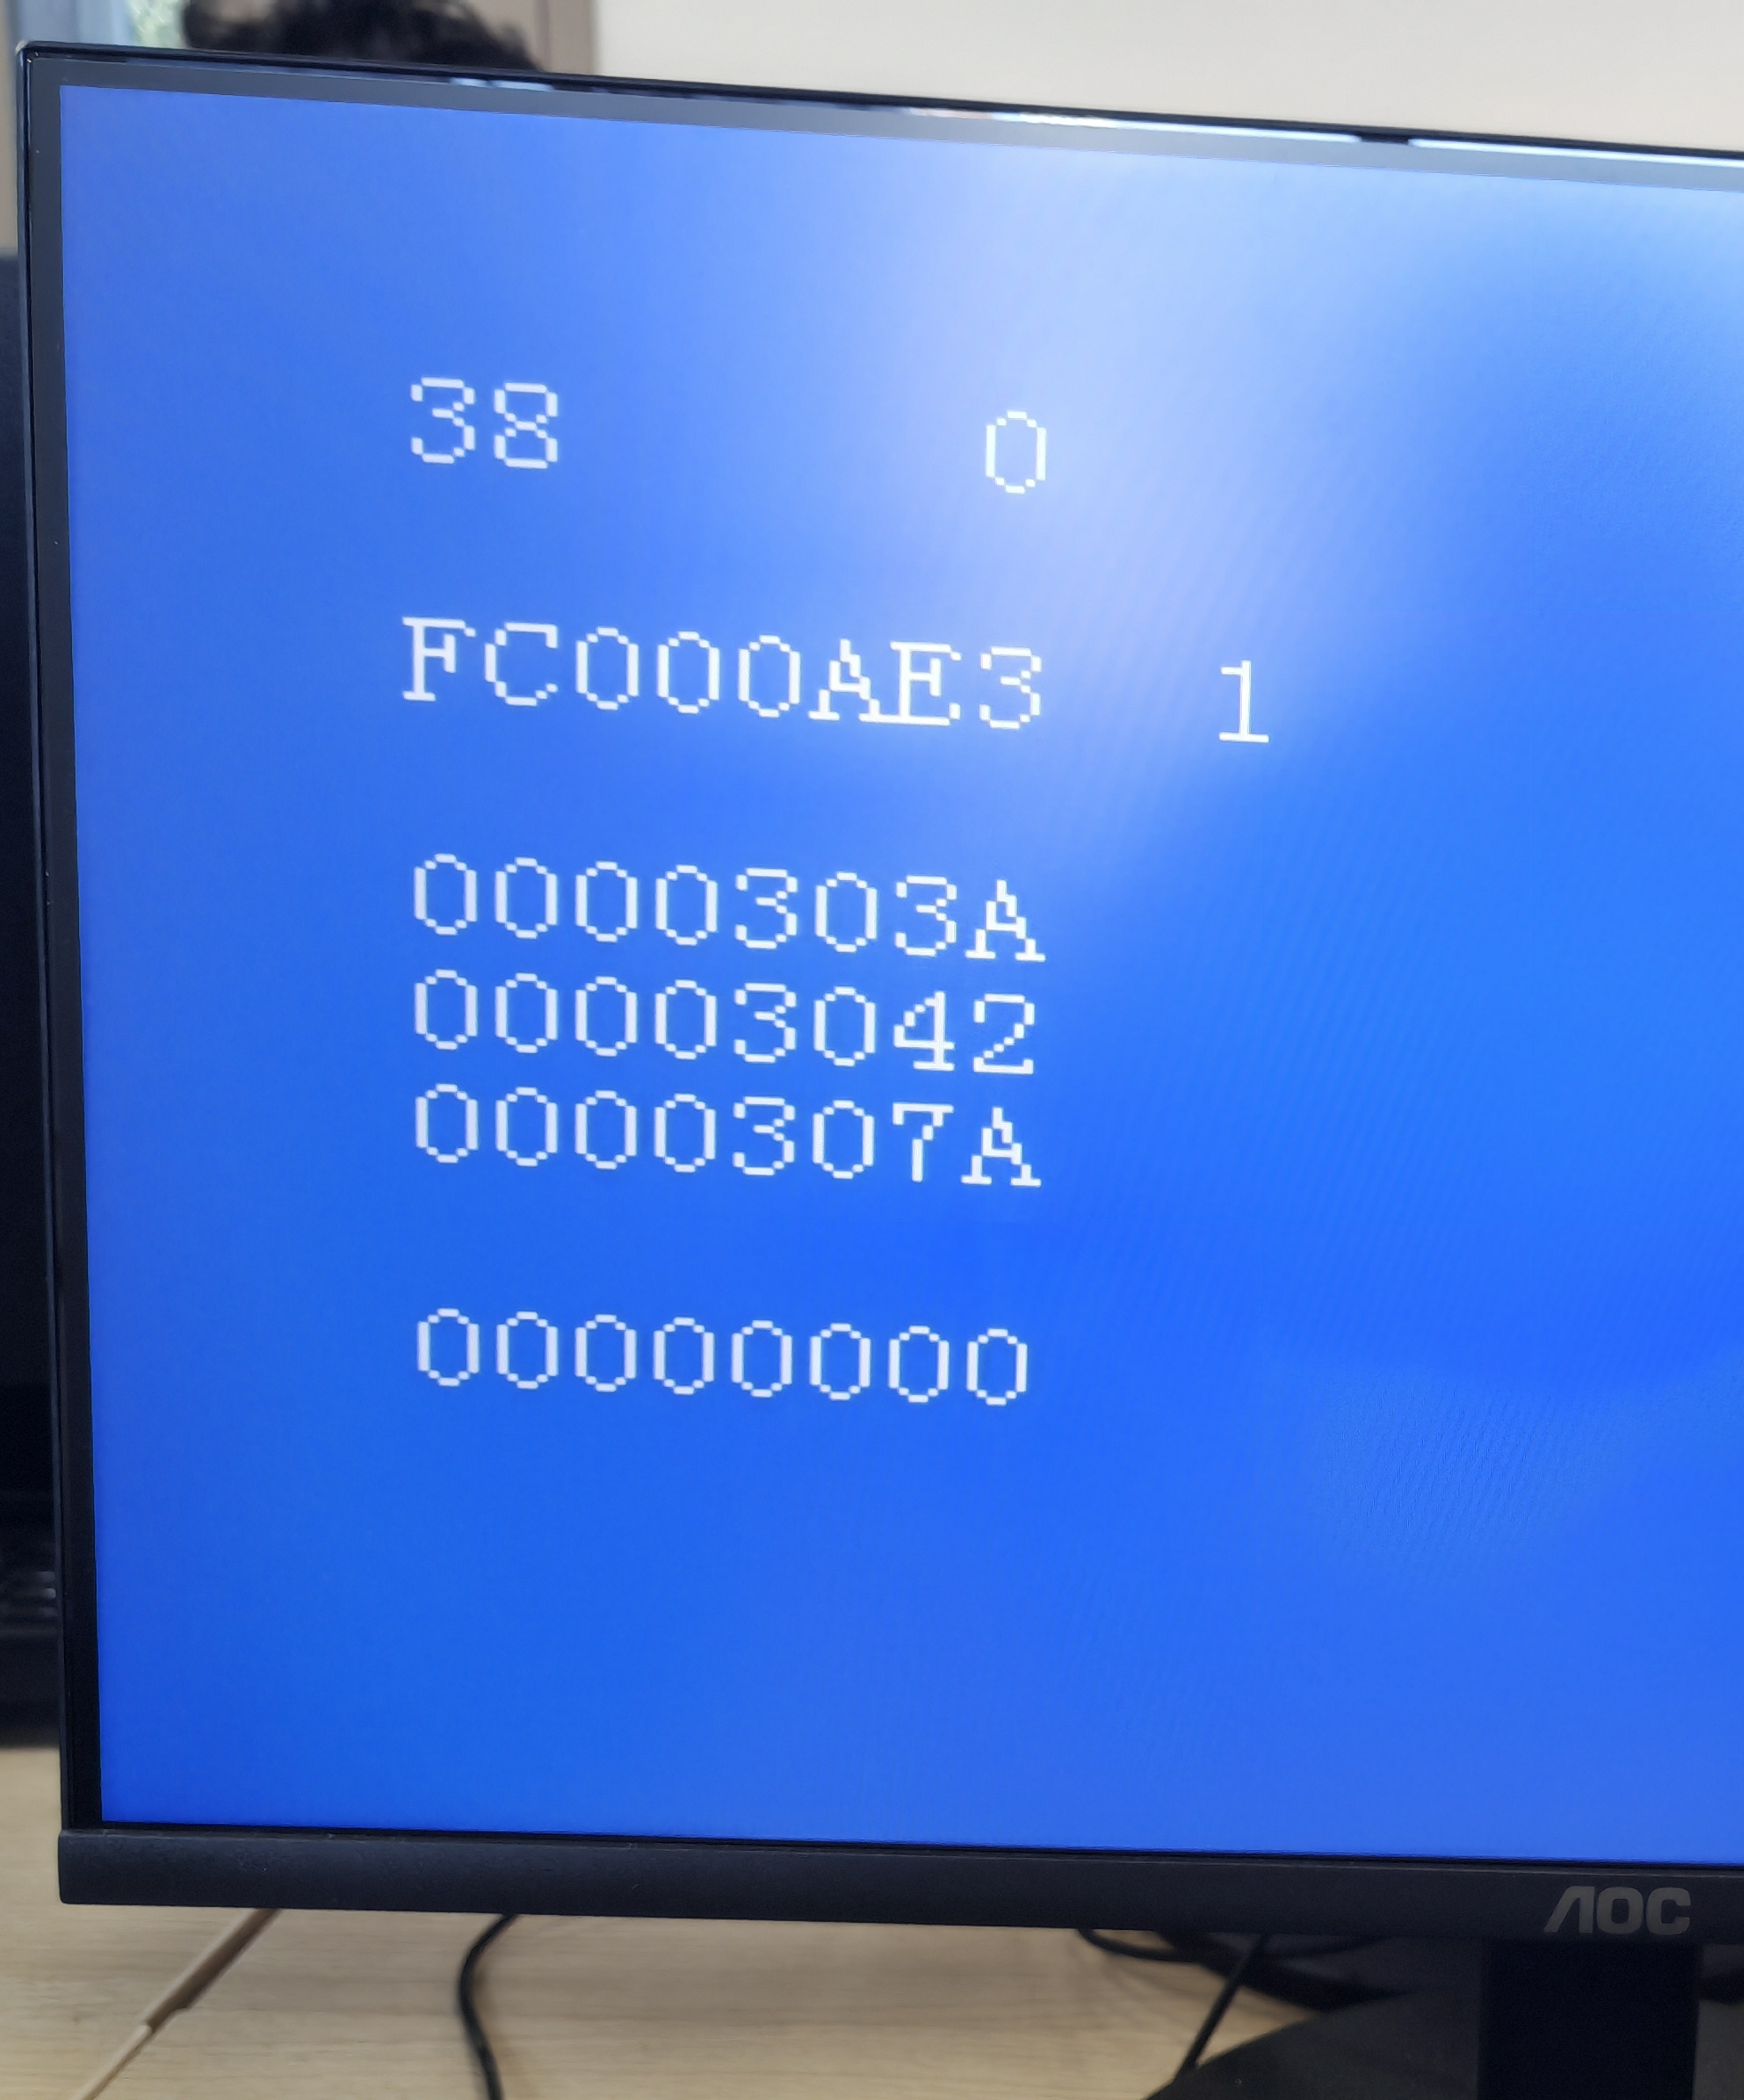
\includegraphics[width=0.4\textwidth]{r2.jpg}
    }
    \subcaptionbox{HDMI显示屏显示内容3}[0.4\textwidth][c]{
        \centering
        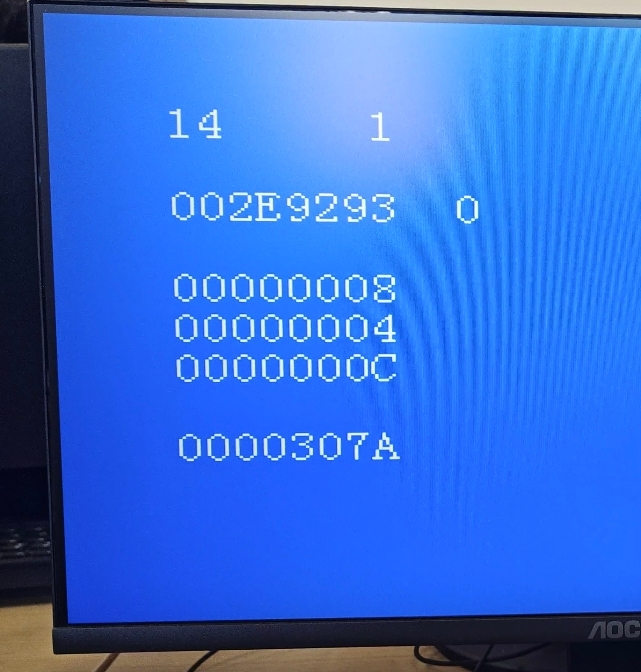
\includegraphics[width=0.4\textwidth]{r3.jpg}
    }%
    \hspace*{0.1cm}
    \subcaptionbox{HDMI显示屏显示内容4}[0.4\textwidth][c]{
        \centering
        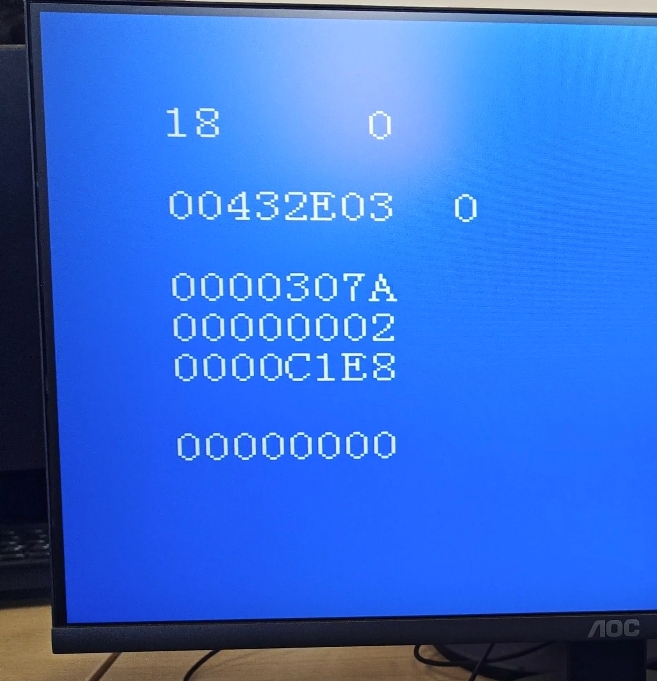
\includegraphics[width=0.4\textwidth]{r4.jpg}
    }%
    \caption{HDMI显示屏显示的部分运行结果}
\end{figure}

\clearpage

\section{拓展部分设计}

\subsection{扩展指令集支持}

要求设计的微处理器还能运行 lb、lh、ld、lbu、lhu、lwu、sb、sh 或 sd 等字节、半字和双字数据传送指令。本设计在 RV32I 架构基础上，增加了对字节（Byte）和半字（Half-word）指令的支持（lb, lh, lbu, lhu, sb, sh）。

\subsubsection{代码修改方案}

为了支持字节和半字操作，我们需要在流水线中传递指令的 \texttt{funct3} 字段，并在 MEM 阶段根据该字段进行数据的截取（Load）或写入位置的调整（Store）。

\begin{enumerate}
    \item \textbf{ID 模块修改 (ID.v)}：
    
    在 ID 模块中增加 \texttt{funct3\_id} 输出端口，直接从指令中提取 \texttt{funct3} 字段（\texttt{Instruction\_id[14:12]}），用于后续阶段判断数据宽度。

\begin{lstlisting}[language=verilog]
module ID(
    // ... (中间端口省略) ...
    output [2:0] funct3_id // 新增端口
);
    // ... (中间代码省略) ...
    
    assign funct3_id = Instruction_id[14:12];

endmodule
\end{lstlisting}

    \item \textbf{Risc5CPU 顶层模块修改 (Risc5CPU.v)}：
    
    \begin{itemize}
        \item \textbf{新增流水线信号}：定义 \texttt{w\_funct3\_id}, \texttt{r\_funct3\_ex}, \texttt{r\_funct3\_mem} 信号，用于在流水线各级间传递 \texttt{funct3}。
        \item \textbf{修改流水线寄存器}：增加 ID/EX 和 EX/MEM 流水线寄存器的位宽，将 \texttt{funct3} 信号传递到 MEM 阶段。
        \item \textbf{Store 逻辑 (MEM 阶段)}：在写入数据存储器前，根据 \texttt{funct3} 和地址低两位（\texttt{ALUResult[1:0]}）修改写入数据。对于 \texttt{sb} 和 \texttt{sh} 指令，采用 "Read-Modify-Write" 的思想（在硬件描述中通过组合逻辑实现），将寄存器中的字节或半字拼接到存储器原有数据的正确位置。
        \item \textbf{Load 逻辑 (MEM 阶段)}：在从数据存储器读出数据后，根据 \texttt{funct3} 和地址低两位进行位扩展。对于 \texttt{lb}/\texttt{lh} 进行符号扩展，对于 \texttt{lbu}/\texttt{lhu} 进行零扩展。
    \end{itemize}

\begin{lstlisting}[language=verilog]
    // Store Logic: Process sb/sh operations
    always @(*) begin
        // Default: sw (Store Word) - write full 32-bit data
        final_ram_write_data = r_MemWriteData_mem;
        
        // sb (Store Byte) - funct3 = 000
        if (r_MemWrite_mem && r_funct3_mem == 3'b000) begin
            case (r_ALUResult_mem[1:0])
                2'b00: final_ram_write_data = {w_MemDout_mem_internal[31:8],  r_MemWriteData_mem[7:0]};
                2'b01: final_ram_write_data = {w_MemDout_mem_internal[31:16], r_MemWriteData_mem[7:0], w_MemDout_mem_internal[7:0]};
                2'b10: final_ram_write_data = {w_MemDout_mem_internal[31:24], r_MemWriteData_mem[7:0], w_MemDout_mem_internal[15:0]};
                2'b11: final_ram_write_data = {r_MemWriteData_mem[7:0],       w_MemDout_mem_internal[23:0]};
            endcase
        end
        // sh (Store Half) - funct3 = 001
        else if (r_MemWrite_mem && r_funct3_mem == 3'b001) begin
            case (r_ALUResult_mem[1]) // Half-word aligned (check bit 1)
                1'b0: final_ram_write_data = {w_MemDout_mem_internal[31:16], r_MemWriteData_mem[15:0]};
                1'b1: final_ram_write_data = {r_MemWriteData_mem[15:0],       w_MemDout_mem_internal[15:0]};
            endcase
        end
    end

    // Load Logic: Process lb/lh/lbu/lhu operations
    always @(*) begin
        // Default: lw (Load Word) - output full RAM data
        final_mem_read_data = w_MemDout_mem_internal;
        
        case (r_funct3_mem)
            3'b000: // lb (Sign Extended Byte)
                case (r_ALUResult_mem[1:0])
                    2'b00: final_mem_read_data = {{24{w_MemDout_mem_internal[7]}},  w_MemDout_mem_internal[7:0]};
                    2'b01: final_mem_read_data = {{24{w_MemDout_mem_internal[15]}}, w_MemDout_mem_internal[15:8]};
                    2'b10: final_mem_read_data = {{24{w_MemDout_mem_internal[23]}}, w_MemDout_mem_internal[23:16]};
                    2'b11: final_mem_read_data = {{24{w_MemDout_mem_internal[31]}}, w_MemDout_mem_internal[31:24]};
                endcase
            3'b001: // lh (Sign Extended Half)
                case (r_ALUResult_mem[1])
                    1'b0: final_mem_read_data = {{16{w_MemDout_mem_internal[15]}}, w_MemDout_mem_internal[15:0]};
                    1'b1: final_mem_read_data = {{16{w_MemDout_mem_internal[31]}}, w_MemDout_mem_internal[31:16]};
                endcase
            3'b100: // lbu (Zero Extended Byte)
                case (r_ALUResult_mem[1:0])
                    2'b00: final_mem_read_data = {24'b0, w_MemDout_mem_internal[7:0]};
                    2'b01: final_mem_read_data = {24'b0, w_MemDout_mem_internal[15:8]};
                    2'b10: final_mem_read_data = {24'b0, w_MemDout_mem_internal[23:16]};
                    2'b11: final_mem_read_data = {24'b0, w_MemDout_mem_internal[31:24]};
                endcase
            3'b101: // lhu (Zero Extended Half)
                case (r_ALUResult_mem[1])
                    1'b0: final_mem_read_data = {16'b0, w_MemDout_mem_internal[15:0]};
                    1'b1: final_mem_read_data = {16'b0, w_MemDout_mem_internal[31:16]};
                endcase
        endcase
    end
\end{lstlisting}
\end{enumerate}

\subsubsection{测试程序设计}

为了验证扩展指令的正确性，设计了如下测试程序（InstructionROM.v）：

\begin{lstlisting}[language=verilog]
// Initialization
addi x1, x0, 0      // Base Addr = 0
addi x2, x0, 0x78   // x2 = 0x78
lui x3, 13          // x3 = 0xD000
addi x3, x3, 0xCDD  // x3 = 0xCCDD

// Store Tests
sb x2, 0(x1)        // Mem[0] = 0x78
sb x2, 1(x1)        // Mem[1] = 0x78
sh x3, 2(x1)        // Mem[2,3] = 0xCCDD
// 预期内存字 (Addr 0): 0xCCDD7878 (Little Endian)

// Load Tests
lb x4, 0(x1)        // x4 = 0x00000078
lb x5, 2(x1)        // x5 = 0xFFFFFFDD (Sign Ext)
lbu x6, 2(x1)       // x6 = 0x000000DD (Zero Ext)
lh x7, 2(x1)        // x7 = 0xFFFFCCDD (Sign Ext)
lhu x8, 2(x1)       // x8 = 0x0000CCDD (Zero Ext)
lw x9, 0(x1)        // x9 = 0xCCDD7878

// Halt
beq x0, x0, 0       // Infinite Loop
\end{lstlisting}

\subsubsection{测试程序运行结果}

下表展示了扩展指令集测试程序在仿真过程中的关键信号变化。需要注意的是，由于流水线的特性，表格中同一行的信号并非来自同一条指令：
\begin{itemize}
    \item \textbf{Instruction (ID)}：当前处于译码阶段的指令。
    \item \textbf{ALU 信号 (EX)}：当前处于执行阶段的指令（即上一条指令）的运算结果。
    \item \textbf{MemDout (MEM)}：当前处于访存阶段的指令（即上上条指令）的读取结果。
\end{itemize}

例如，在 Clk=6 时，ID 阶段为 \texttt{sb x2, 0(x1)} 指令，而 EX 阶段正在执行上一条 \texttt{addi x3, x3, 0xCDD} 指令，因此 ALU 输出为 \texttt{0xD000 + 0xFFFFFCDD = 0xCCDD}。

\begin{table}[H]
\centering
\caption{扩展指令集测试程序运行结果对照表}
\label{tab:ext_test_result}
\renewcommand{\arraystretch}{1.2} % 增加行高
\setlength{\tabcolsep}{4pt} % 调整列间距
\resizebox{\textwidth}{!}{%
\begin{tabular}{|c|c|c|c|c|c|c|c|c|c|}
\hline
\rowcolor{gray!20} \textbf{clk} & \textbf{PC} & \textbf{Instruction (ID)} & \textbf{JumpFlag} & \textbf{Stall} & \textbf{ALU\_A} & \textbf{ALU\_B} & \textbf{ALUResult} & \textbf{MemDout (MEM)} & \textbf{RegWriteData (WB)} \\ \hline
... & ... & ... & ... & ... & ... & ... & ... & ... & ... \\ \hline
6 & 14 & 00208023 (sb) & 0 & 0 & 0000d000 & fffffcdd & 0000ccdd & - & - \\ \hline
7 & 18 & 002080a3 (sb) & 0 & 0 & 00000000 & 00000000 & 00000000 & - & - \\ \hline
8 & 1c & 00309123 (sh) & 0 & 0 & 00000000 & 00000001 & 00000001 & - & - \\ \hline
9 & 20 & 00008203 (lb) & 0 & 0 & 00000000 & 00000002 & 00000002 & - & - \\ \hline
10 & 24 & 00208283 (lb) & 0 & 0 & 00000000 & 00000000 & 00000000 & - & - \\ \hline
11 & 28 & 0020c303 (lbu) & 0 & 0 & 00000000 & 00000002 & 00000002 & ccdd7878 & - \\ \hline
12 & 2c & 00209383 (lh) & 0 & 0 & 00000000 & 00000002 & 00000002 & ccdd7878 & 00000078 \\ \hline
13 & 30 & 0020d403 (lhu) & 0 & 0 & 00000000 & 00000002 & 00000002 & ccdd7878 & ffffffdd \\ \hline
14 & 34 & 0000a483 (lw) & 0 & 0 & 00000000 & 00000002 & 00000002 & ccdd7878 & 000000dd \\ \hline
15 & 38 & 00000063 (beq) & 1 & 0 & 00000000 & 00000000 & 00000000 & ccdd7878 & ffffccdd \\ \hline
16 & 38 & 00000063 (beq) & 0 & 0 & 00000000 & 00000000 & 00000000 & ccdd7878 & 0000ccdd \\ \hline
17 & 38 & 00000063 (beq) & 1 & 0 & 00000000 & 00000000 & 00000000 & ccdd7878 & ccdd7878 \\ \hline

\end{tabular}%
}
\end{table}

\subsubsection{仿真结果验证}

仿真波形如下图所示。

\begin{figure}[H]
    \centering
    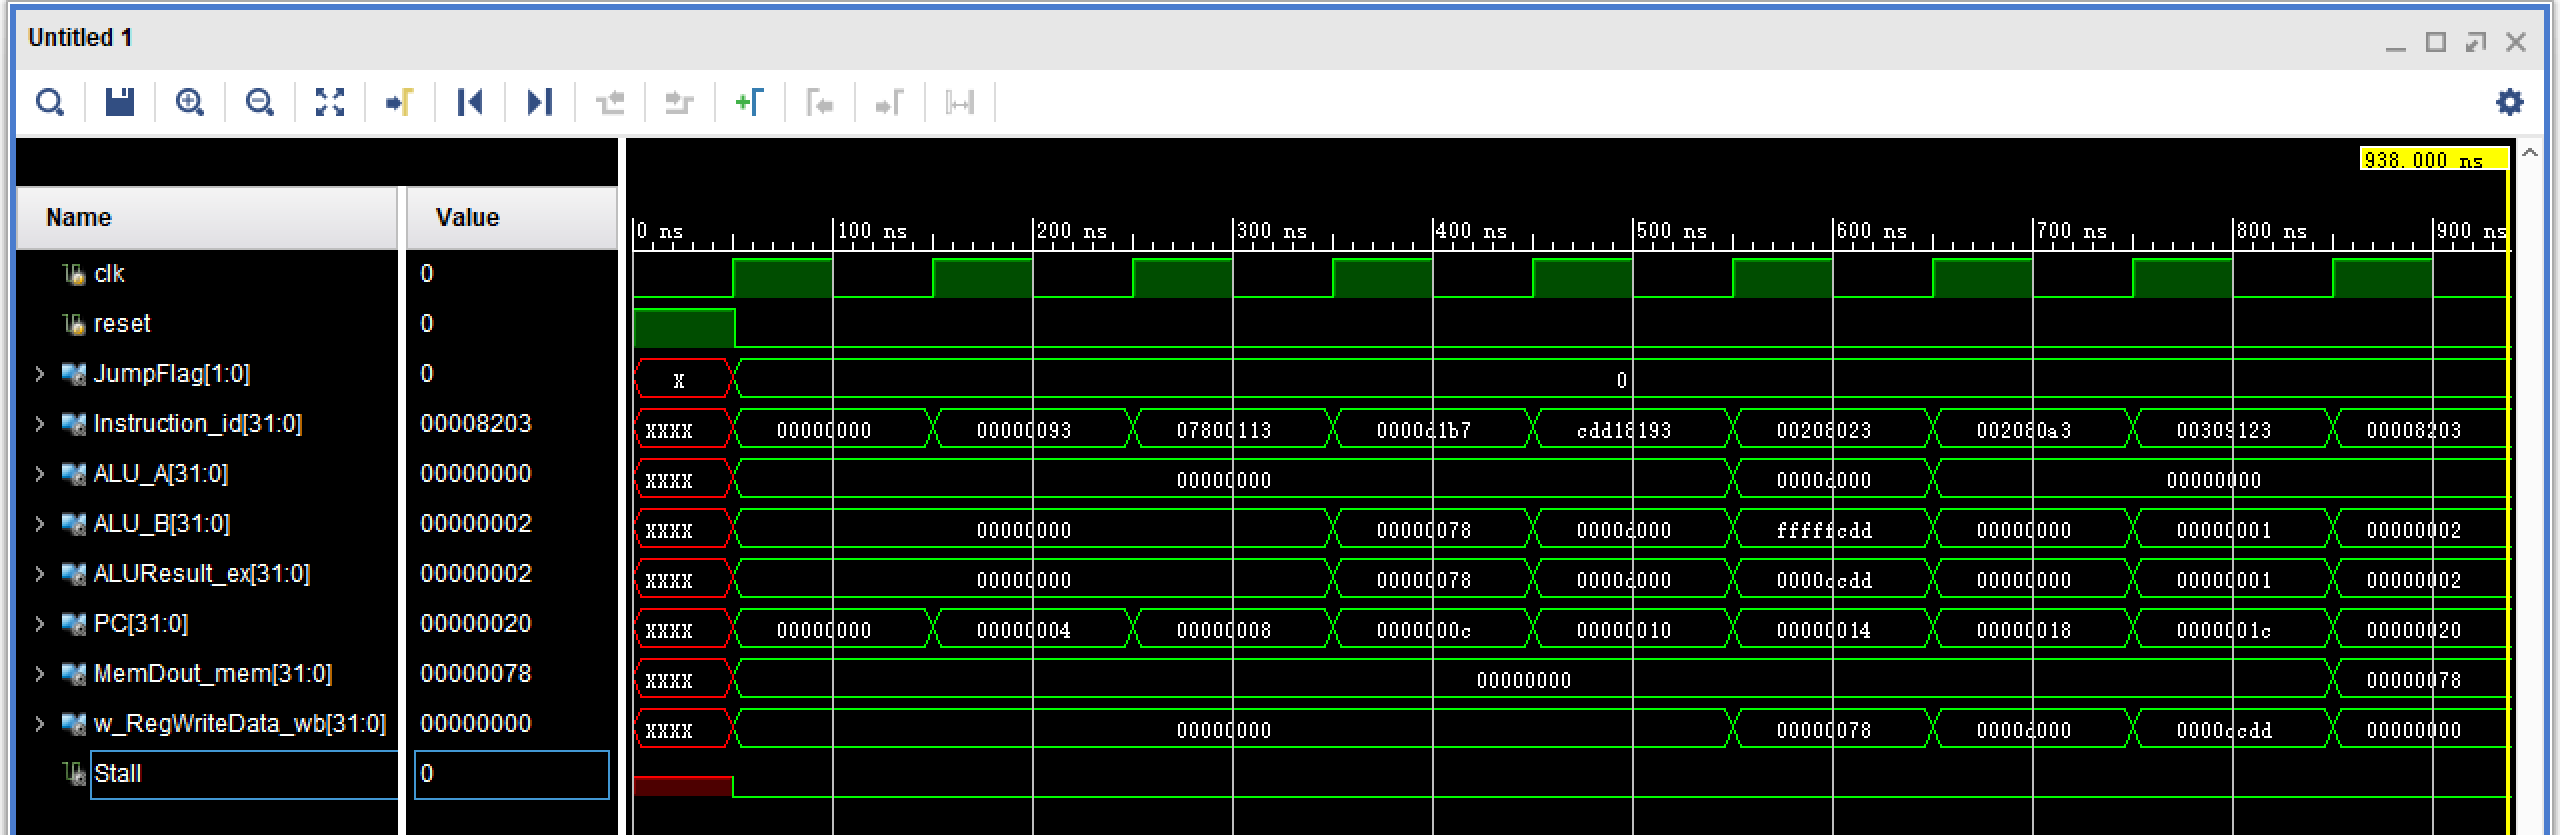
\includegraphics[width=1\textwidth]{p7.png}
    \caption{扩展指令集仿真波形1}
\end{figure}

\begin{figure}[H]
    \centering
    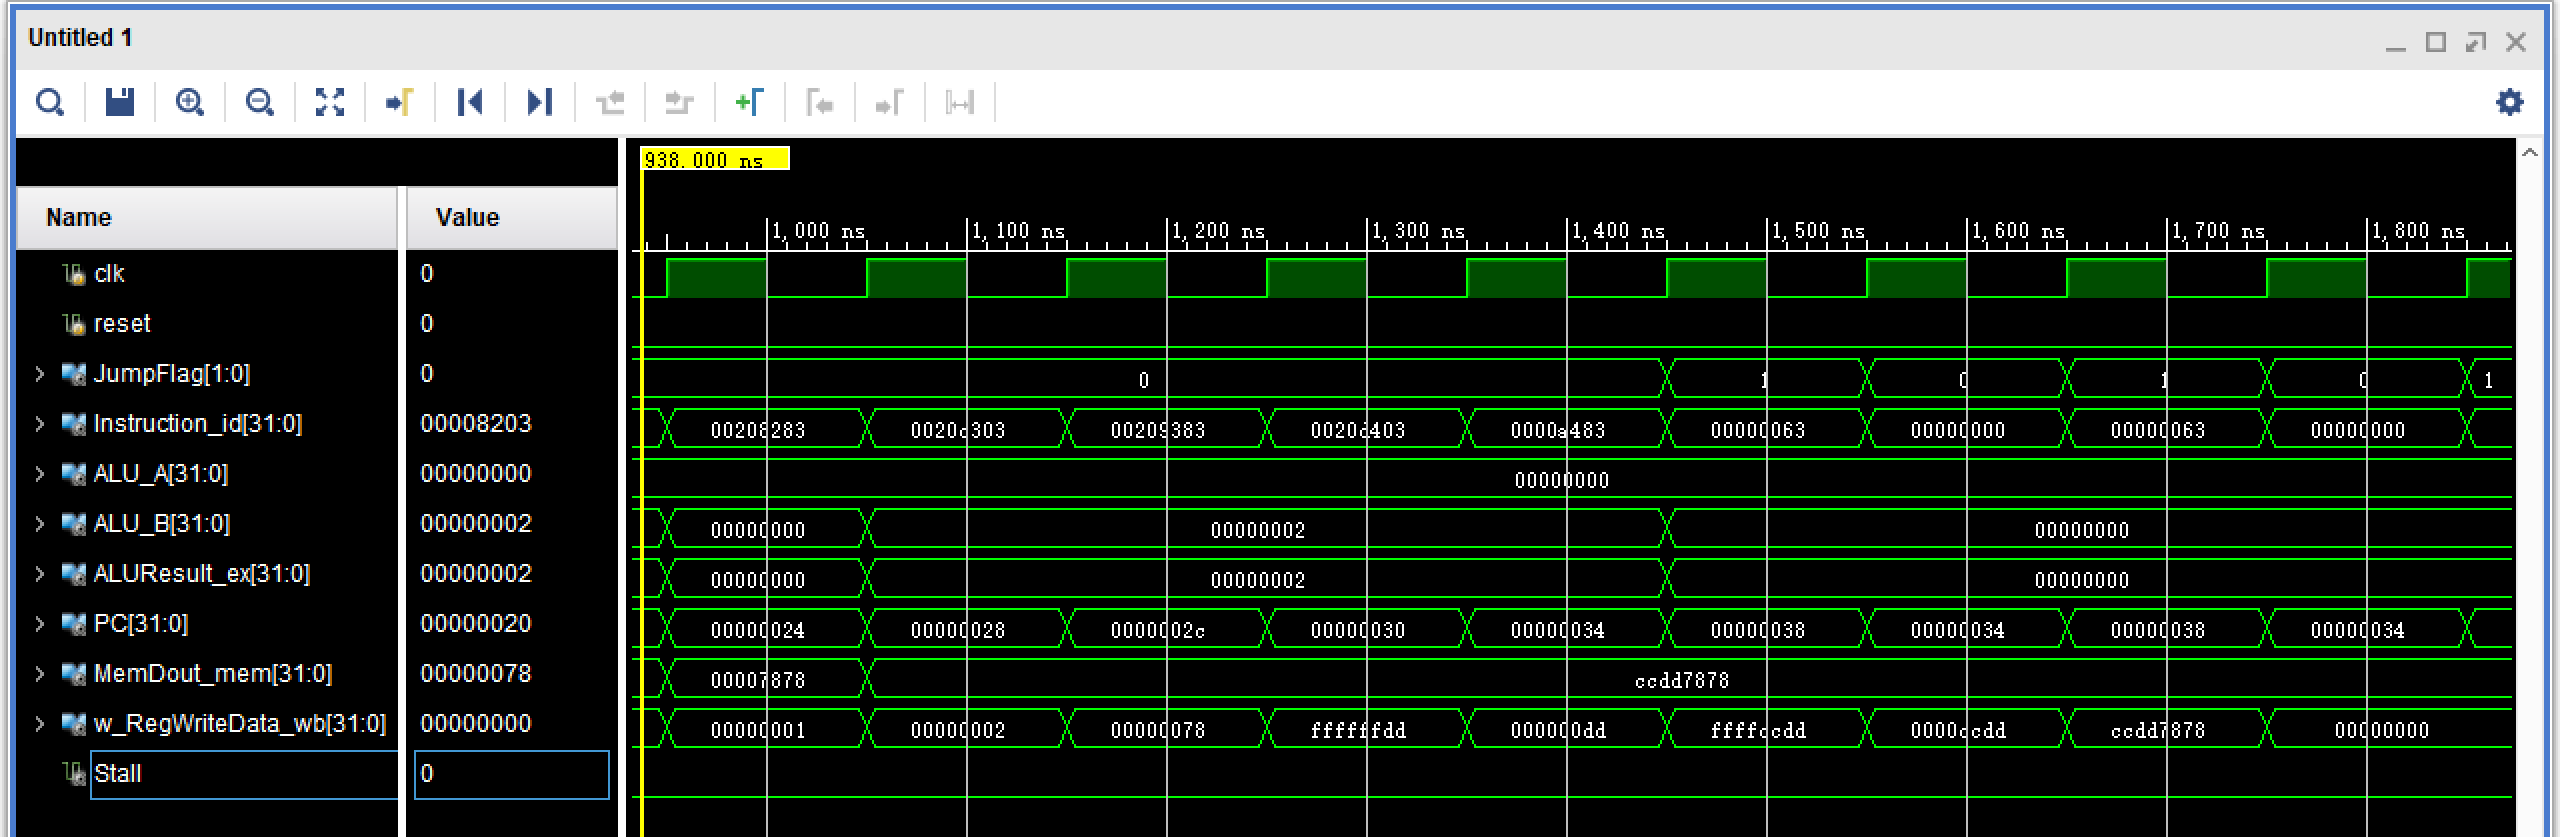
\includegraphics[width=1\textwidth]{p8.png}
    \caption{扩展指令集仿真波形2}
\end{figure}

\textbf{结果分析：}

从波形图中可以观察到：
\begin{enumerate}
    \item \textbf{Store 操作验证}：在执行完 \texttt{sb} 和 \texttt{sh} 指令后，当执行 \texttt{lw x9, 0(x1)} 时，\texttt{MemDout} 输出为 \texttt{0xccdd7878}。这表明内存地址 0 和 1 被正确写入了 \texttt{0x78}，地址 2 和 3 被正确写入了 \texttt{0xCCDD}。
    \item \textbf{Load 操作验证}：
    \begin{itemize}
        \item \texttt{lb x4, 0(x1)} 结果为 \texttt{0x00000078}，正确读取字节。
        \item \texttt{lb x5, 2(x1)} 结果为 \texttt{0xffffffdd}，正确读取字节并进行了符号扩展（\texttt{0xDD} 最高位为 1）。
        \item \texttt{lbu x6, 2(x1)} 结果为 \texttt{0x000000dd}，正确读取字节并进行了零扩展。
        \item \texttt{lh x7, 2(x1)} 结果为 \texttt{0xffffccdd}，正确读取半字并进行了符号扩展。
        \item \texttt{lhu x8, 2(x1)} 结果为 \texttt{0x0000ccdd}，正确读取半字并进行了零扩展。
        \item \texttt{lw x9, 0(x1)} 结果为 \texttt{0xccdd7878}，正确读取完整字（4字节），验证了之前 \texttt{sb} 和 \texttt{sh} 指令的写入结果。
    \end{itemize}
\end{enumerate}

仿真结果与预期完全一致，证明微处理器已正确支持字节和半字的数据传送指令。

\clearpage
\subsection{异常处理机制}

要求设计的 CPU 增加异常（exception）、自陷（trap）、中断（interrupt）等处理方案。

\subsubsection{代码修改方案}

\begin{enumerate}
    \item \textbf{CSR模块设计 (CSR.v)}：

    新增 CSR.v，支持 mtvec、mepc、mcause、mstatus 等寄存器的读写，处理异常入口和返回。CSR 读写接口如下：

\begin{lstlisting}[language=verilog]
module CSR(
    input clk, input reset,
    input [11:0] csr_addr,
    input [31:0] csr_wdata,
    input [1:0]  csr_op,      // 00: Read, 01: Write, 10: Set, 11: Clear
    output reg [31:0] csr_rdata,
    input trap_en, input mret_en,
    input [31:0] pc_in, input [31:0] cause_in,
    output [31:0] trap_pc_out, epc_out, mcause_out
);
// ... 省略 ...
endmodule
\end{lstlisting}

    \item \textbf{指令译码与异常检测 (Decode.v, ID.v)}：

    \begin{itemize}
        \item \textbf{Decode.v}：增加 SYSTEM 指令类型，解析 CSR 操作、ECALL、MRET、非法指令等信号。
        \item \textbf{ID.v}：实例化 CSR 模块，处理异常入口（Trap）、返回（MRET）和 CSR 读写，输出调试端口。
    \end{itemize}

\begin{lstlisting}[language=verilog]
// Decode.v 片段
parameter SYSTEM_op = 7'b1110011;
assign CSR_op = SYSTEM ? (
    (funct3 == 3'b001) ? 2'b01 : // CSRRW
    (funct3 == 3'b010) ? 2'b10 : // CSRRS
    (funct3 == 3'b011) ? 2'b11 : // CSRRC
    2'b00 ) : 2'b00;
assign ECALL = SYSTEM & (funct3 == 3'b000) & (Instruction[31:20] == 12'd0);
assign MRET  = SYSTEM & (funct3 == 3'b000) & (Instruction[31:20] == 12'h302);
assign Illegal = ~(R_type | I_type | ... | SYSTEM);
\end{lstlisting}

\begin{lstlisting}[language=verilog]
// ID.v 片段
CSR u_CSR (
    .clk(clk), .reset(reset),
    .csr_addr(Instruction_id[31:20]),
    .csr_wdata(rs1Data_id),
    .csr_op(CSR_op),
    .csr_rdata(csr_rdata),
    .trap_en(Trap), .mret_en(MRET),
    .pc_in(PC_id), .cause_in(Illegal ? 32'd2 : 32'd11),
    .trap_pc_out(trap_pc), .epc_out(epc), .mcause_out(Debug_mcause)
);
assign JumpAddr = Trap ? trap_pc : (MRET ? epc : JumpAddr_decode);
assign Jump = Jump_decode | Trap | MRET;
assign Imm_id = (CSR_op != 0) ? csr_rdata : Imm_decode;
\end{lstlisting}

    \item \textbf{顶层模块与流水线寄存器 (Risc5CPU.v)}：
   
    异常相关信号：顶层输出 Debug\_mepc、Debug\_mcause、Debug\_mtvec 便于仿真和调试。

\begin{lstlisting}[language=verilog]
module Risc5CPU(
    input clk,
    input reset,
    //... 原有信号省略
    output [31:0] Debug_mepc,
    output [31:0] Debug_mcause,
    output [31:0] Debug_mtvec
);
\end{lstlisting}

\clearpage
\subsubsection{测试程序设计}

 设计了包含非法指令、ECALL、异常返回等指令的测试程序，验证异常处理流程。为解决流水线数据冒险，合理插入 NOP。

\begin{lstlisting}[language=verilog]
// Setup Handler
6'd0:  dout=32'h04000093; // addi x1, x0, 0x40
6'd1:  dout=32'h00000013; // nop
6'd2:  dout=32'h00000013; // nop
6'd3:  dout=32'h30509073; // csrw mtvec, x1
// Test Illegal Instruction
6'd4:  dout=32'hFFFFFFFF; // Illegal Instruction
// Test ECALL
6'd6:  dout=32'h00000073; // ecall
// Exception Handler
6'd16: dout=32'h34202F73; // csrr x30, mcause
6'd17: dout=32'h34102FF3; // csrr x31, mepc
6'd18: dout=32'h00000013; // nop
6'd19: dout=32'h00000013; // nop
6'd20: dout=32'h004F8F93; // addi x31, x31, 4
6'd21: dout=32'h00000013; // nop
6'd22: dout=32'h00000013; // nop
6'd23: dout=32'h341F9073; // csrw mepc, x31
6'd24: dout=32'h30200073; // mret
\end{lstlisting}

\end{enumerate}

\subsubsection{仿真与验证}

基于 Vivado 仿真波形（如图 \ref{fig:trap_sim_1} 至图 \ref{fig:trap_sim_3} 所示），我们可以观察到处理器在遇到异常时的精确行为。以下针对仿真过程中的四个关键跳转与反跳转阶段进行详细分析：

\subsubsection{非法指令异常触发（PC $14 \to 40$）}
如图 \ref{fig:trap_sim_1} 所示，在仿真时间 700ns 附近：
\begin{itemize}
    \item \textbf{状态分析}：此时 ID 阶段正在译码地址为 \texttt{32'h10} 的指令 \texttt{0xFFFFFFFF}。由于这是一条未定义的非法指令，Decoder 模块输出 \texttt{Illegal} 信号，导致 \texttt{Trap} 信号有效。
    \item \textbf{PC行为}：由于流水线的预取机制，此时 IF 阶段的 PC 寄存器值已经更新为下一条指令的地址 \texttt{32'h14}。
    \item \textbf{CSR更新}：\texttt{Trap} 信号触发 CSR 模块更新：
    \begin{itemize}
        \item \texttt{Debug\_mcause} 更新为 \texttt{32'h2}，对应 RISC-V 标准中的 "Illegal instruction"。
        \item \texttt{Debug\_mepc} 锁存当前导致异常的指令地址，即 \texttt{32'h10}。
    \end{itemize}
    \item \textbf{跳转结果}：下一时钟周期，PC 并没有继续执行 \texttt{0x14}，而是被强制跳转到 \texttt{Debug\_mtvec} 指定的异常入口地址 \texttt{32'h40}。这验证了异常入口逻辑的正确性。
\end{itemize}

\begin{figure}[H]
    \centering
    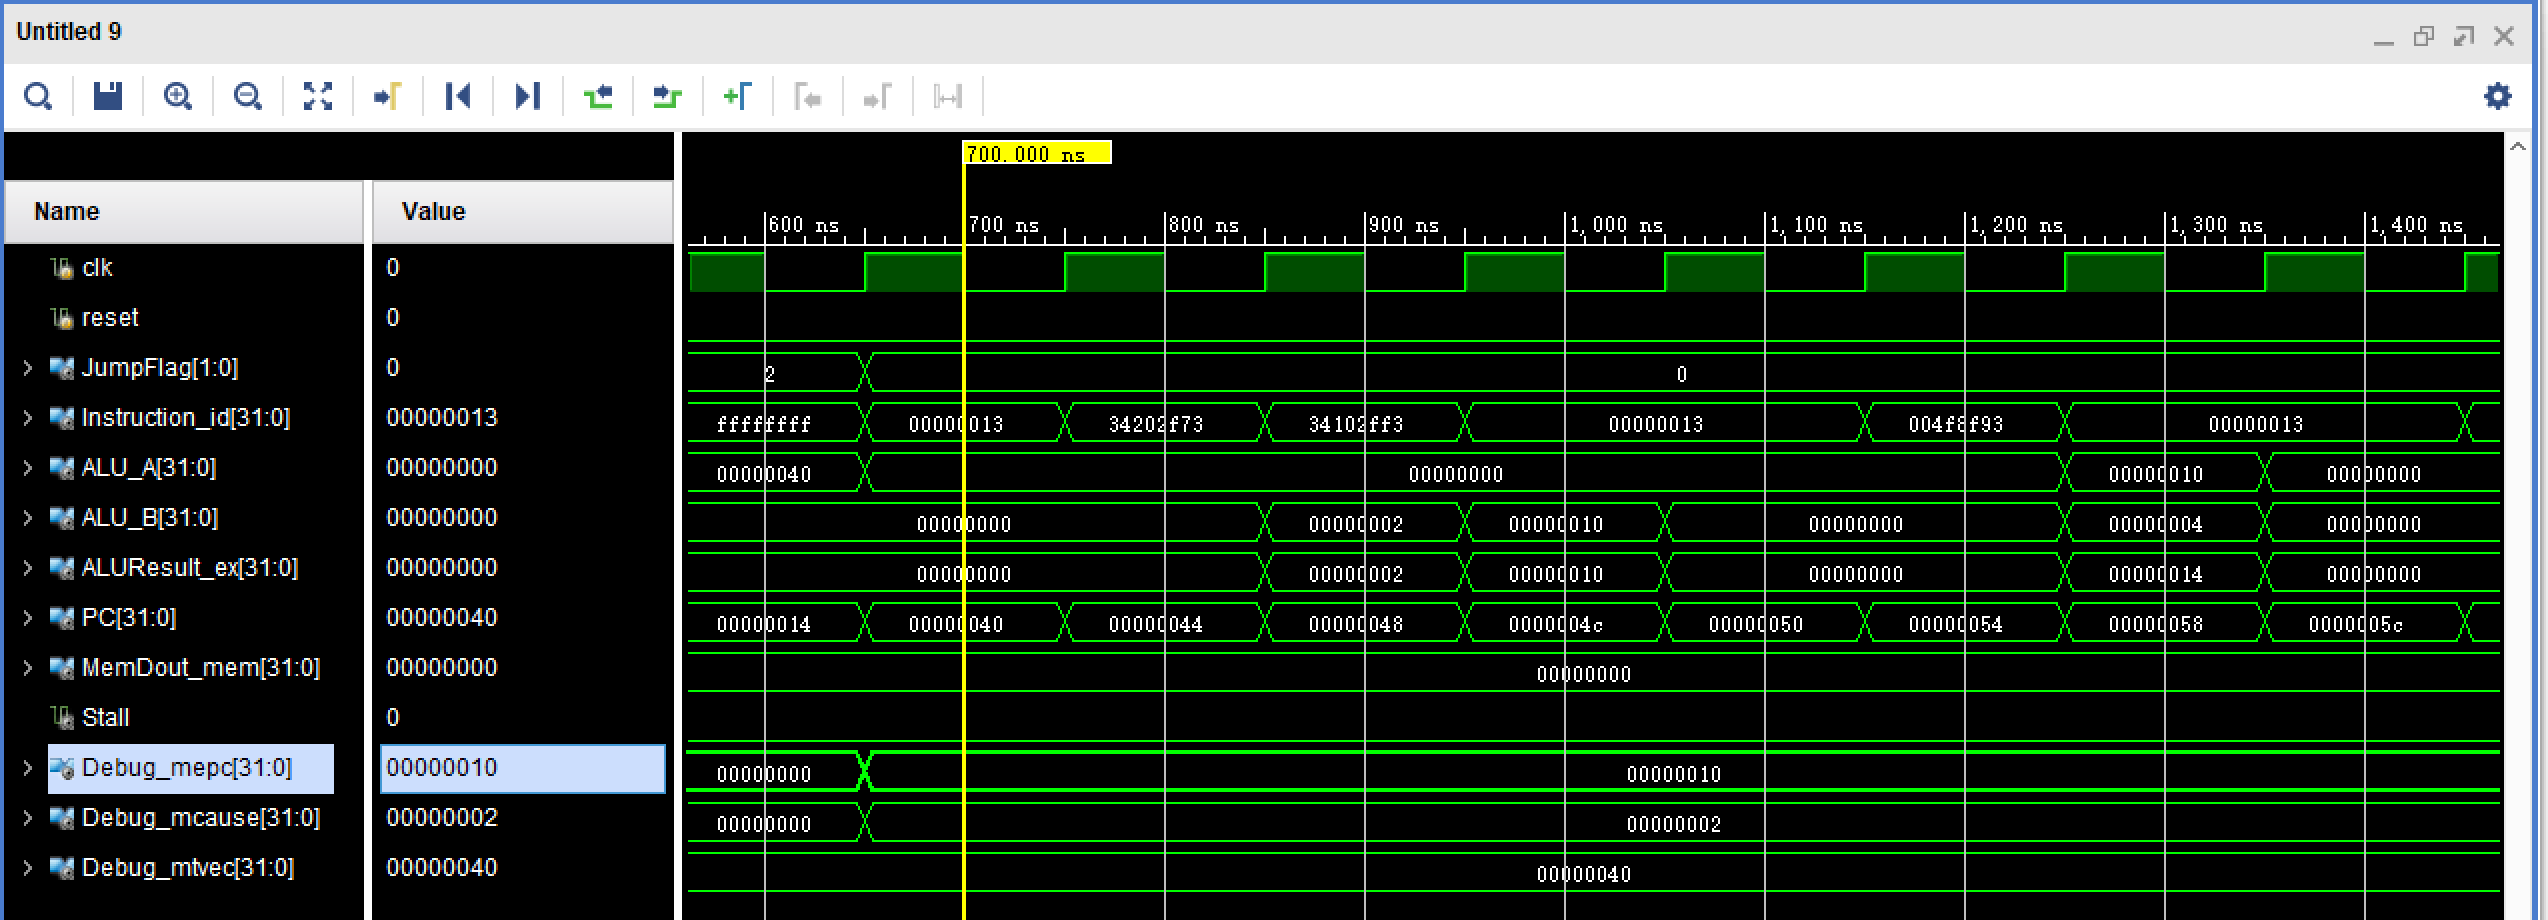
\includegraphics[width=1\textwidth]{p10.png}
    \caption{非法指令异常触发仿真波形}
    \label{fig:trap_sim_1}
\end{figure}

\subsubsection{非法指令异常返回（PC $64 \to 14$）}
如图 \ref{fig:trap_sim_2} 左侧所示，在仿真时间 1700ns 附近：
\begin{itemize}
    \item \textbf{状态分析}：异常处理程序（位于地址 \texttt{0x40} - \texttt{0x60}）执行完毕。处理程序通过指令计算将 \texttt{mepc} 的值加 4（即 $10 + 4 = 14$），以跳过错误的指令，并将结果 \texttt{32'h14} 写回 \texttt{Debug\_mepc}。
    \item \textbf{MRET指令}：处理器执行位于 \texttt{0x60} 的 \texttt{mret} 指令。此时由于流水线预取，PC 显示为 \texttt{32'h64}。
    \item \textbf{CSR读取}：\texttt{mret} 指令使能 \texttt{MRET} 信号，处理器从 \texttt{CSR} 模块读取 \texttt{epc\_out}。
    \item \textbf{跳转结果}：PC 从 \texttt{32'h64} 跳转回 \texttt{Debug\_mepc} 的当前值 \texttt{32'h14}。这意味着 CPU 成功从异常处理程序返回，并准确跳过了之前的非法指令，开始执行地址 \texttt{0x14} 处的代码。
\end{itemize}

\begin{figure}[H]
    \centering
    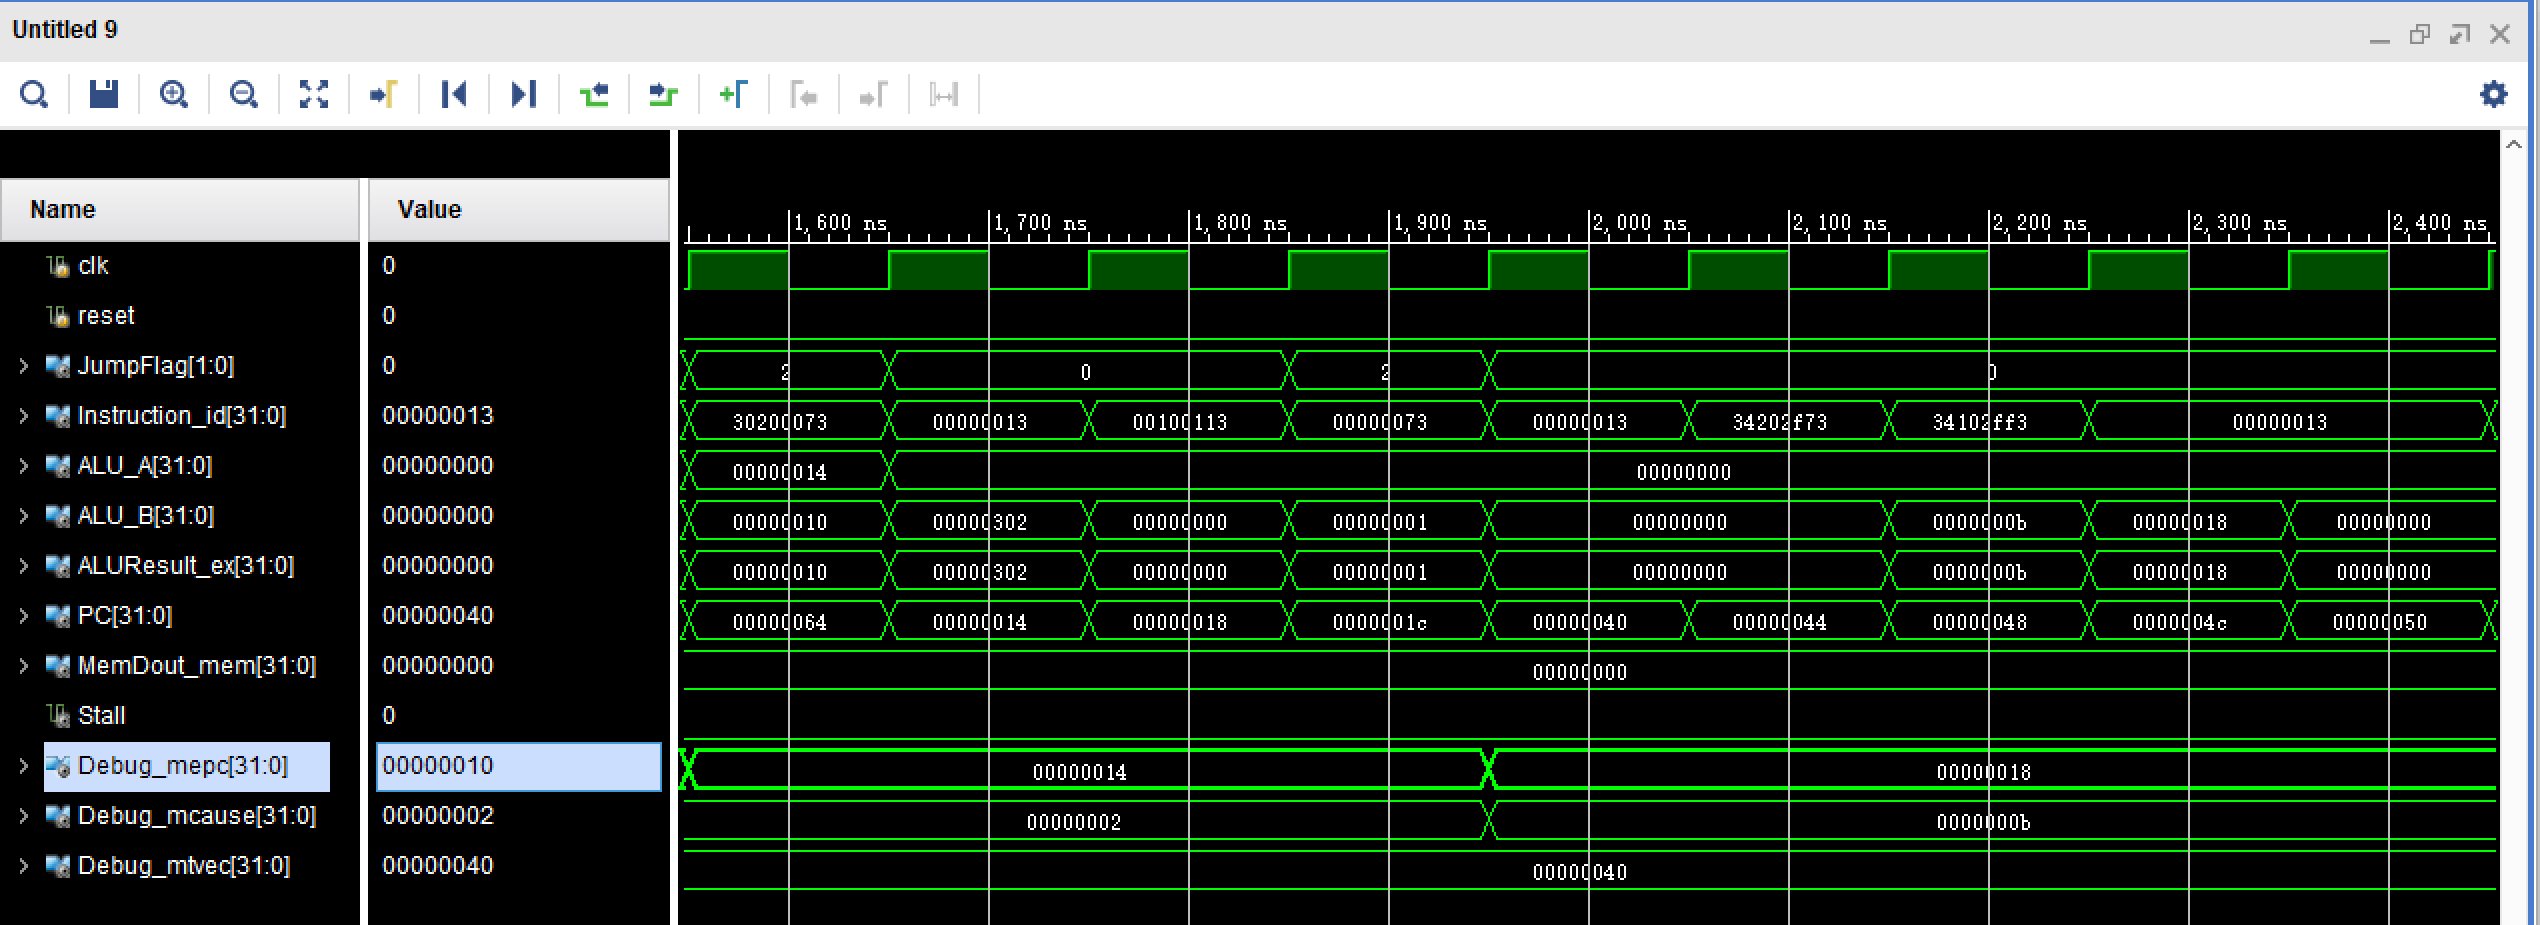
\includegraphics[width=1\textwidth]{p11.png}
    \caption{异常返回与ECALL触发仿真波形}
    \label{fig:trap_sim_2}
\end{figure}

\subsubsection{ECALL异常触发（PC $1C \to 40$）}
如图 \ref{fig:trap_sim_2} 中部所示，在仿真时间 1900ns 附近：
\begin{itemize}
    \item \textbf{状态分析}：程序顺序执行到地址 \texttt{32'h18}，此处为 \texttt{ecall} 指令（机器码 \texttt{00000073}）。ID 模块译码检测到系统调用。
    \item \textbf{PC行为}：此时 IF 阶段的 PC 已经预取了下一条地址 \texttt{32'h1C}。
    \item \textbf{CSR更新}：\texttt{Trap} 再次触发：
    \begin{itemize}
        \item \texttt{Debug\_mcause} 更新为 \texttt{32'hB}（即十进制 11），对应 "Environment call from M-mode"。
        \item \texttt{Debug\_mepc} 锁存当前 \texttt{ecall} 指令的地址 \texttt{32'h18}。
    \end{itemize}
    \item \textbf{跳转结果}：PC 从 \texttt{32'h1C} 再次强制跳转到异常入口 \texttt{32'h40}，进入处理程序。
\end{itemize}

\subsubsection{ECALL异常返回（PC $64 \to 1C$）}
如图 \ref{fig:trap_sim_3} 所示，在仿真时间 3200ns 附近：
\begin{itemize}
    \item \textbf{状态分析}：异常处理程序再次运行。它读取 \texttt{mepc}（此时为 \texttt{0x18}），将其加 4 得到 \texttt{0x1C}，并写回 \texttt{mepc}。这确保返回后执行 \texttt{ecall} 之后的下一条指令。
    \item \textbf{跳转结果}：执行 \texttt{mret} 指令时，PC 当前值为 \texttt{32'h64}（预取值）。处理器读取更新后的 \texttt{Debug\_mepc} 值 \texttt{32'h1C}，并完成跳转。
    \item \textbf{验证结论}：波形显示 PC 成功跳转至 \texttt{32'h1C}，\texttt{Debug\_mcause} 保持为 \texttt{0xB}（直到下一次异常改变它），\texttt{Debug\_mepc} 稳定在 \texttt{0x1C}。这证明了 CPU 正确处理了自陷指令并成功返回到了预期的程序断点。
\end{itemize}

\begin{figure}[H]
    \centering
    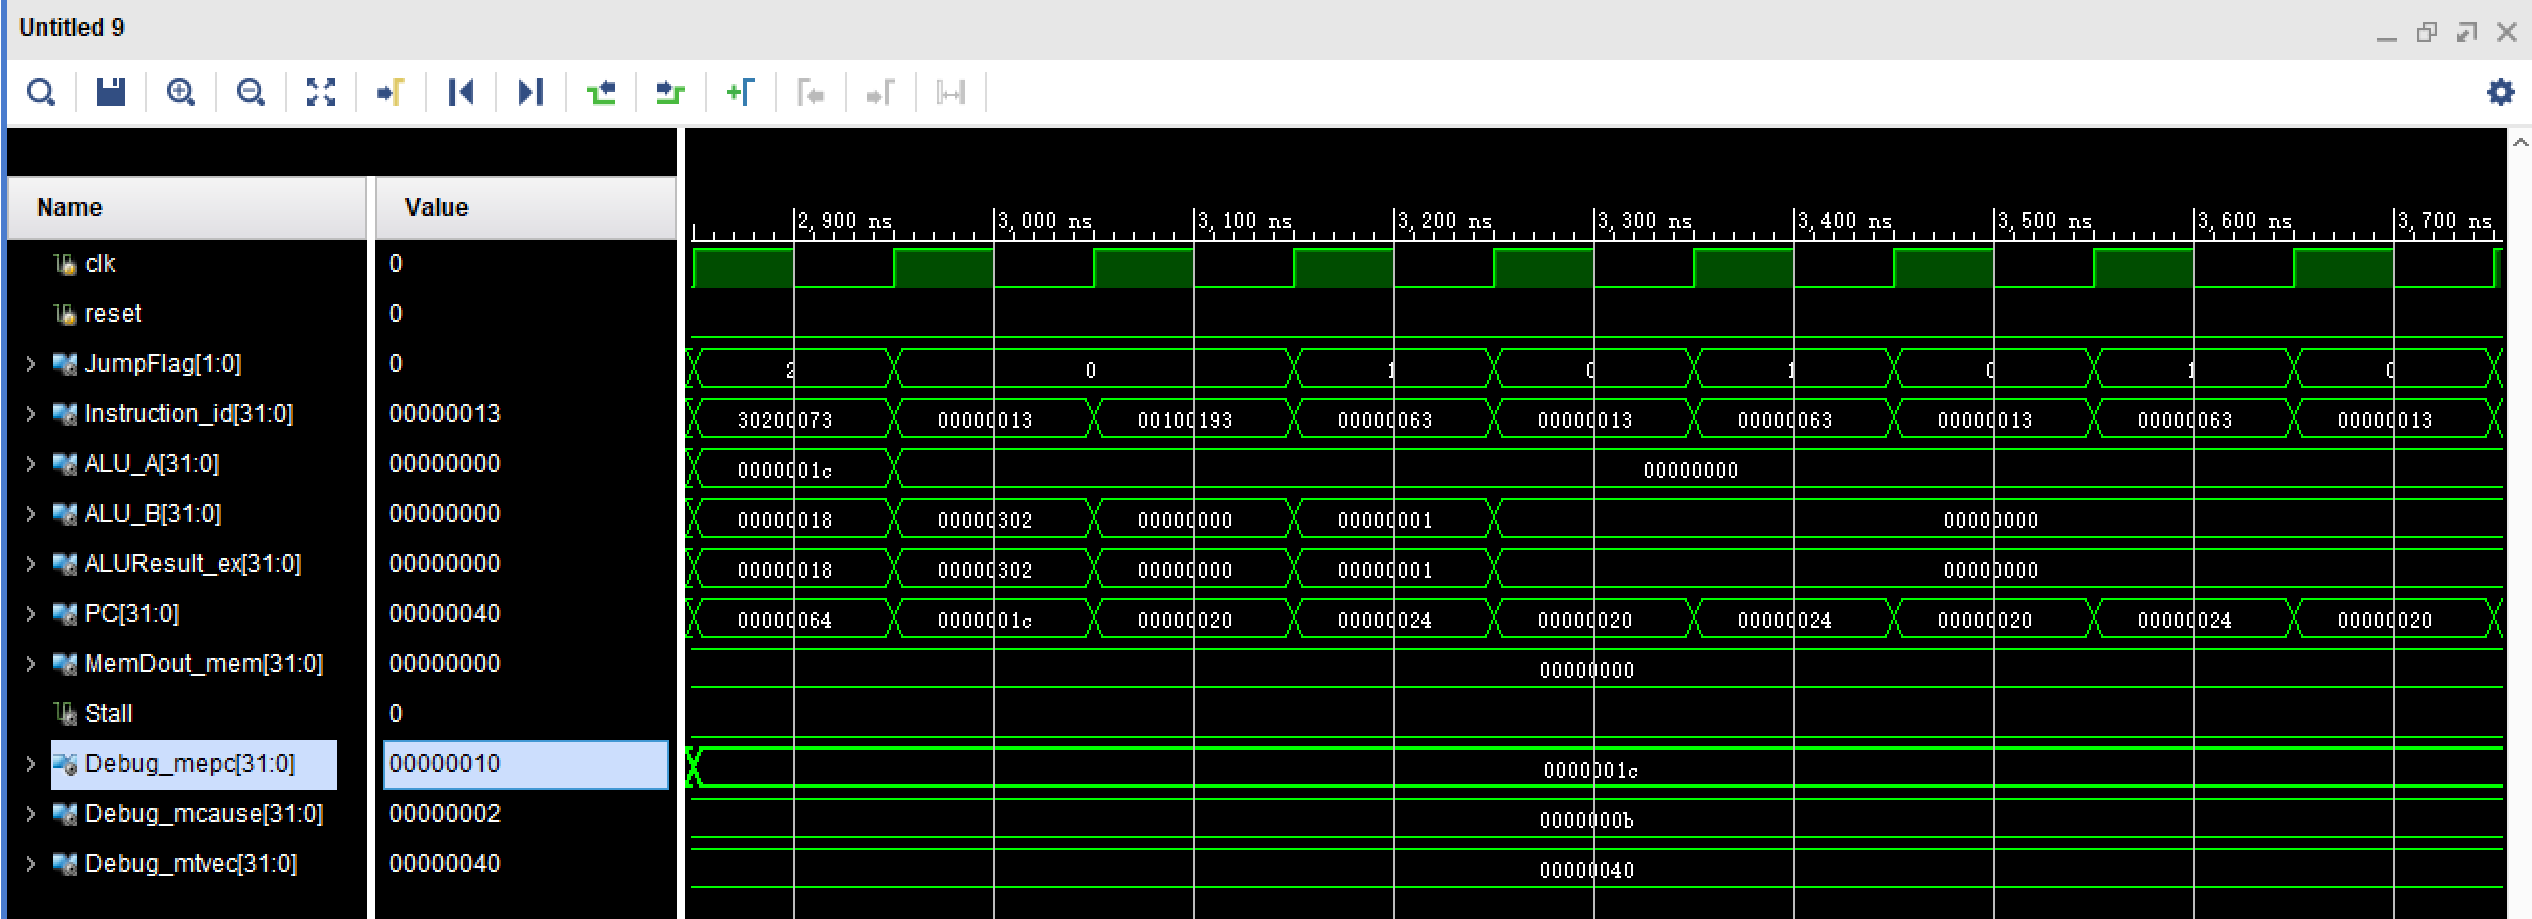
\includegraphics[width=1\textwidth]{p12.png}
    \caption{ECALL异常返回仿真波形}
    \label{fig:trap_sim_3}
\end{figure}

\subsubsection{结论}

在标准 RV32I 流水线架构的基础上，成功集成了 CSR 控制状态寄存器堆与异常处理逻辑。通过对非法指令（Illegal Instruction）和系统调用（ECALL）的仿真验证，得出以下结论：

\begin{enumerate}
    \item \textbf{异常响应机制正确}：CPU 能够准确识别译码阶段的异常源，并立即触发生流水线冲刷（Flush），将下一条指令地址强制指向 \texttt{mtvec} 设定的异常入口地址（0x40），实现了硬件级的控制流切换。
    \item \textbf{上下文保存准确}：在异常触发周期，CSR 模块能够正确且自动地将异常原因写入 \texttt{mcause}（非法指令为 2，ECALL 为 11），并将受害指令地址锁存至 \texttt{mepc}，为异常处理程序提供了准确的现场信息。
    \item \textbf{返回机制有效}：\texttt{mret} 指令能够正确读取 \texttt{mepc} 寄存器的值并装载至 PC，且仿真表明异常处理程序对 \texttt{mepc} 的软件修改（+4操作）能够正确生效，确保了 CPU 在异常返回后能够执行正确的下一条指令，避免了死循环。
    \item \textbf{CSR读写功能正常}：除了硬件自动更新外，指令集对 CSR 寄存器的读写指令（csrr/csrw）功能正常，满足了软硬件协同处理异常的需求。
\end{enumerate}

综上所述，本设计成功扩展了 RISC-V 处理器的特权级架构，具备了精确异常处理（Precise Exception Handling）能力，完全达到了实验扩展要求中关于异常与自陷处理的设计指标。
\clearpage
\section{遇到问题与解决}

\subsection{Vivado 2017.3 Implementation 阶段卡死问题}

在使用 Vivado 2017.3 打开文件夹下的vivado201701进行 FPGA 综合和实现时，出现了 Synthesis 阶段成功完成，但在 Implementation 阶段卡死在 "Initializing Design" 步骤的情况。具体表现为：

\begin{itemize}
    \item Synthesis 综合过程正常完成，无错误或警告
    \item 点击 Run Implementation 后，进度条停留在 "Initializing Design" 阶段
    \item 查看 Log 文件发现没有任何新的输出信息
    \item 进程长时间无响应，CPU 和内存占用也无明显变化
\end{itemize}

\textbf{问题分析：}

经过多次尝试和观察，初步判断这是 Vivado 2017.3 版本的稳定性问题。该版本在处理某些设计时可能会出现内部状态异常，导致 Implementation 工具链无法正常启动或卡死。

\textbf{解决方法：}

更换版本为Vivado 2017.4，问题解决

\clearpage
\section{思考题}

如下面两条指令，条件分支指令试图读取上一条指令的目标寄存器，插入气泡或数据转发都无法解决流水线冲突问题。为什么在大多 CPU 架构中，都不去解决这一问题？这一问题应在什么层面中解决？

\begin{lstlisting}[language={[x86masm]Assembler}]
lw   X28, 04(X6)
beq  X28, X29, Loop
\end{lstlisting}

\subsection{问题分析：}

这是一个load-use 数据冒险与分支指令结合的问题。lw 指令在 MEM 阶段才能获得数据，而 beq 指令需要在 ID 阶段就进行分支判断和比较，此时 lw 指令还未完成数据加载。

\textbf{为什么大多 CPU 架构不在硬件层面解决：}

\begin{enumerate}
    \item \textbf{硬件复杂度过高}：若要在硬件层面完全解决，有两种可能的方案：
    
    \textbf{方案一：}将分支判断延迟到 EX 或 MEM 阶段，这会导致：
    \begin{itemize}
        \item 分支预测失败的代价增加（更多指令需要被冲刷）
        \item 控制逻辑和数据通路变得更加复杂
        \item 关键路径延长，降低时钟频率
    \end{itemize}
    
    \textbf{方案二：}添加专门的硬件单元来提前加载数据，这也会显著增加硬件资源消耗和设计复杂度。
    
    \item \textbf{发生频率较低}：这种特定的冒险场景（load 后紧跟依赖该数据的分支）在实际程序中出现频率相对较低，不值得为此大幅增加硬件复杂度。
\end{enumerate}

\subsection{解决方案}

这一问题应在编译器层面解决：
    \begin{itemize}
        \item \textbf{指令调度}：编译器在生成代码时，识别这种冒险，在 lw 和 beq 之间插入一条无关指令（如其他运算），利用指令级并行性。
        \item \textbf{延迟槽}：某些架构（如 MIPS）显式定义延迟槽，要求编译器填充有用的指令或 nop。
        \item \textbf{代码重排}：将分支判断所需的 load 指令提前，与分支指令保持足够距离。
    \end{itemize}

\subsection{硬件设计尝试}
\subsubsection{实现思路}
修改 Hazard\_Detector 模块，使其能够识别“Load 指令在 MEM 阶段 且 当前是 Branch 指令”的情况，并强制再阻塞一个周期。这需要引入 MemRead\_mem 和 rdAddr\_mem 信号回传到 ID 阶段。

这种策略能综合考虑了硬件资源与性能开销，仅增加了一个周期的延迟，同时避免了复杂的硬件设计。
\subsubsection{代码修改方案}

为了在硬件层面解决 Load 指令后紧跟分支指令（Load-Branch Hazard）产生的冲突，我们需要强制流水线在现有的 Load-Use 阻塞基础上再阻塞一个周期。这涉及到三个模块的修改：\texttt{Hazard\_Detector}、\texttt{ID} 和顶层 \texttt{Risc5CPU}。

\textbf{1. 冒险检测模块修改 (Hazard\_Detector.v)}

修改核心逻辑，增加对 MEM 阶段 Load 指令的检测。如果 MEM 阶段是 Load 指令，且其目标寄存器与当前 ID 阶段分支指令的源寄存器冲突，则产生阻塞。

\begin{lstlisting}[language=verilog]
module Hazard_Detector(
    // ... 输入输出端口定义 ...
    input MemRead_mem,      // 新增：MEM阶段的读使能
    input [4:0] rdAddr_mem, // 新增：MEM阶段的目标寄存器
    input [31:0] Instruction_id // 新增：用于判断是否为分支指令
);

    // 1. 判断当前 ID 阶段是否为分支指令
    wire IsBranch = (Instruction_id[6:0] == 7'b1100011);

    // 2. 原有的检测：Load 在 EX 阶段 (需要第 1 个 Stall)
    wire Hazard_EX = MemRead_ex && ((rdAddr_ex == rs1Addr_id) || 
                     (rdAddr_ex == rs2Addr_id)) && (rdAddr_ex != 0);

    // 3. 新增检测：Load 在 MEM 阶段 (需要第 2 个 Stall)
    // 仅当当前指令是 Branch 时才需要，因为 Branch 在 ID 阶段就需要数据
    wire Hazard_MEM = MemRead_mem && ((rdAddr_mem == rs1Addr_id) || 
                      (rdAddr_mem == rs2Addr_id)) && (rdAddr_mem != 0) && IsBranch;

    // 4. 只要满足任一条件，就阻塞
    assign Stall = Hazard_EX | Hazard_MEM;
    assign IFWrite = ~Stall;

endmodule
\end{lstlisting}

\textbf{2. ID 模块修改 (ID.v)}

在 ID 模块增加接收 MEM 阶段信号的端口，并将其传递给实例化的冒险检测模块。

\begin{lstlisting}[language=verilog]
module ID(
    // ... 原有端口 ...
    input MemRead_mem,      // 新增输入
    input [4:0] rdAddr_mem  // 新增输入
);
    // ... 中间代码 ...

    // 实例化 Hazard_Detector 时连接新信号
    Hazard_Detector u_Hazard_Detector (
        .MemRead_ex(MemRead_ex),
        .rdAddr_ex(rdAddr_ex),
        .MemRead_mem(MemRead_mem), // 连接新增信号
        .rdAddr_mem(rdAddr_mem),   // 连接新增信号
        .Instruction_id(Instruction_id),
        // ... 其他连接 ...
    );
endmodule
\end{lstlisting}

\textbf{3. 顶层模块修改 (Risc5CPU.v)}

这是最关键的一步，需要定义 MEM 阶段的控制信号，并确保 \texttt{MemRead} 信号通过流水线寄存器正确传递到 MEM 阶段，最后连接回 ID 模块。

\begin{lstlisting}[language=verilog]
// 1. 定义信号
wire r_MemRead_mem; // 定义 MEM 阶段的读信号

// 2. 修改 EX/MEM 流水线寄存器，增加位宽并传输 MemRead 信号
DFF #(.WIDTH(76)) u_reg_EX_MEM ( // 位宽从 75 增加到 76
    .clk(clk),
    .reset(reset),
    .clear(1'b0),
    .en(1'b1),
    // 输入端增加 r_MemRead_ex
    .d({w_ALUResult_ex_internal, w_MemWriteData_ex,
        r_MemWrite_ex, r_RegWrite_ex, r_MemtoReg_ex, r_MemRead_ex, ...}), 
    // 输出端增加 r_MemRead_mem
    .q({r_ALUResult_mem, r_MemWriteData_mem,
        r_MemWrite_mem, r_RegWrite_mem, r_MemtoReg_mem, r_MemRead_mem, ...})
);

// 3. 修改 ID 模块实例化，连接反馈信号
ID u_ID (
    // ... 原有连接 ...
    .MemRead_mem(r_MemRead_mem), // 将 MEM 阶段信号回传给 ID
    .rdAddr_mem(r_rdAddr_mem),
    // ...
);
\end{lstlisting}

\subsubsection{仿真与验证}

为了验证上述硬件修改的有效性，我们编写了专门的测试程序如下，并在 Vivado 中进行了仿真。核心测试逻辑为：先将寄存器 \texttt{x5} 置为错误值（99），然后执行 \texttt{lw x5, 4(x1)} 加载正确值（5），紧接着执行 \texttt{beq x5, x2, PASS}。如果冒险解决，分支应跳转；否则分支失败。

\begin{lstlisting}[language=verilog]
module InstructionROM(addr, dout);
    input [5 : 0] addr;
    output [31 : 0] dout;
    reg [31 : 0] dout;

    always @(*)
        case (addr)
            6'd0:  dout = 32'h00000093; // addi x1, x0, 0      (基址 = 0)
            6'd1:  dout = 32'h00500113; // addi x2, x0, 5      (预期值 = 5)
            6'd2:  dout = 32'h06300293; // addi x5, x0, 99     (x5置脏 = 99)
            6'd3:  dout = 32'h0020a223; // sw x2, 4(x1)        (Mem[4] = 5)
            
            // --- 冒险测试区 ---
            6'd4:  dout = 32'h0040a283; // lw x5, 4(x1)        (加载 Mem[4] 到 x5)
            6'd5:  dout = 32'h00228663; // beq x5, x2, PASS    (若 x5==5 跳转至 addr 8)
            
            // --- 失败分支 ---
            6'd6:  dout = 32'hbad00513; // addi x10, x0, 0xBAD
            6'd7:  dout = 32'h00000463; // beq x0, x0, DONE    (跳转至结束)

            // --- 成功分支 ---
            6'd8:  dout = 32'h00100513; // addi x10, x0, 1

            // --- 结束停机 ---
            6'd9:  dout = 32'h00000063; // beq x0, x0, 0       (死循环)

            default: dout = 32'h00000013; // nop
        endcase
endmodule
\end{lstlisting}

\begin{figure}[H]
    \centering
    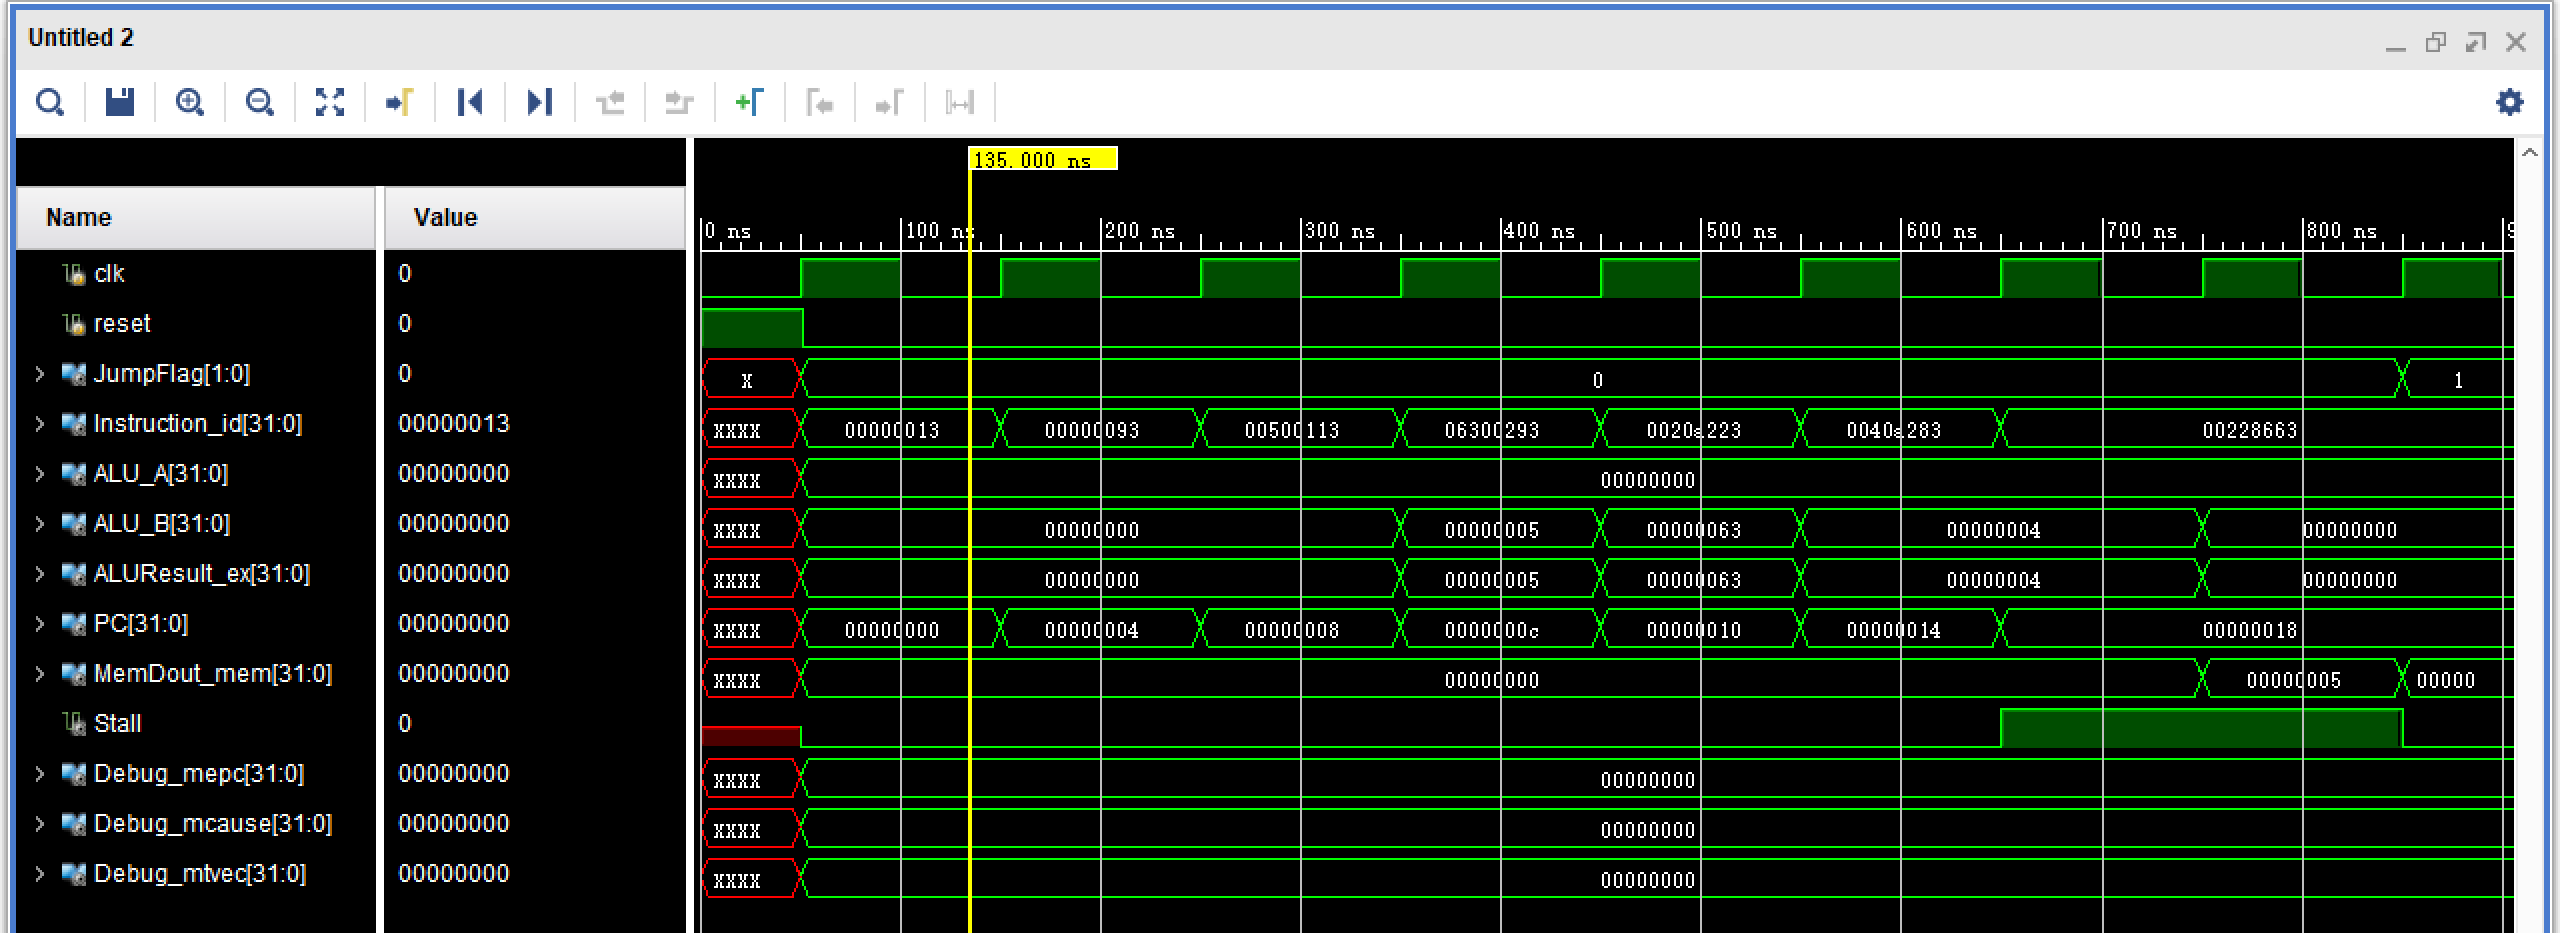
\includegraphics[width=1\textwidth]{p13.png}
    \caption{Load-Branch 冒险测试整体仿真波形}
    \label{fig:hazard_sim_full}
\end{figure}

\begin{figure}[H]
    \centering
    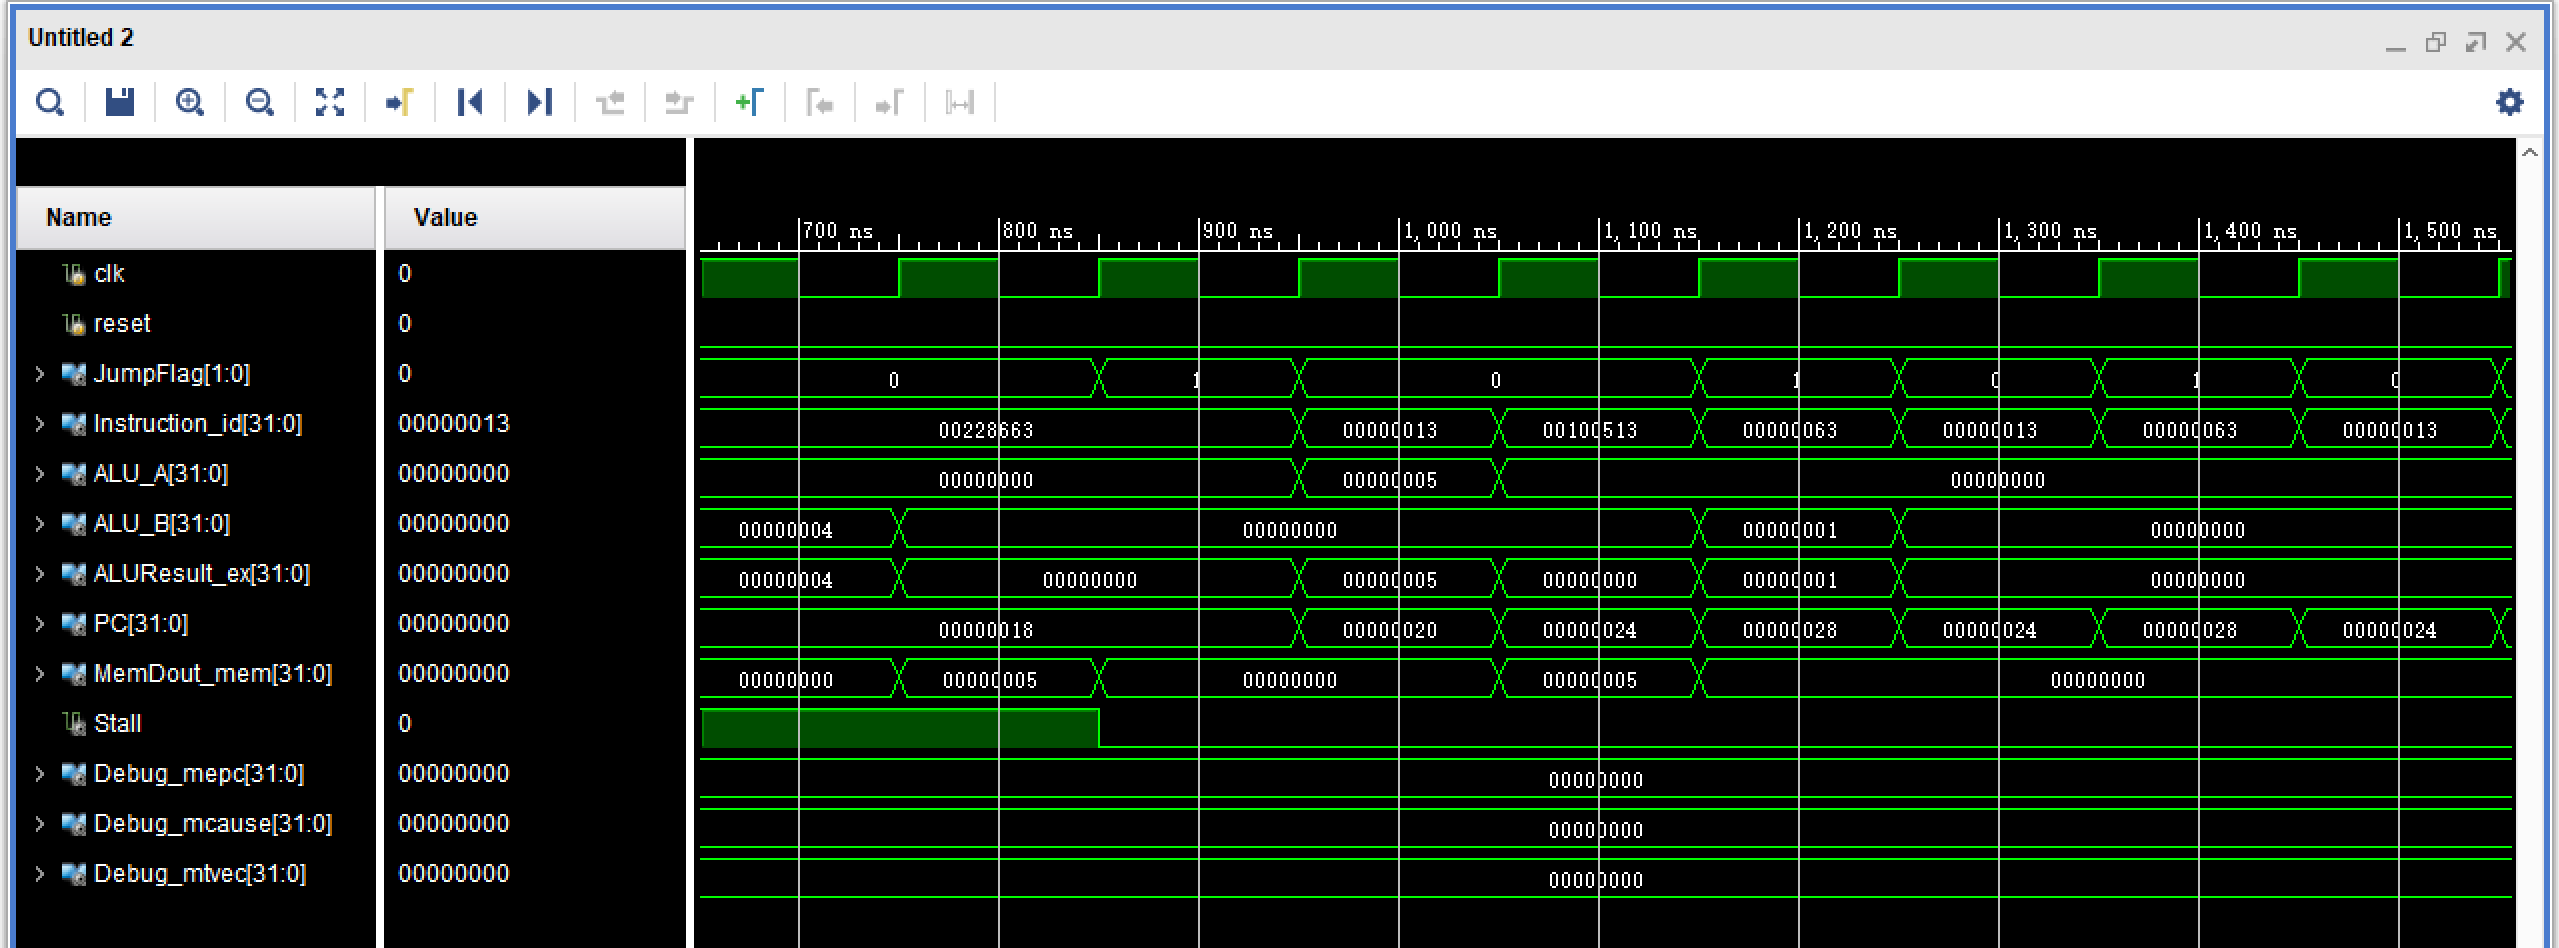
\includegraphics[width=1\textwidth]{p14.png}
    \caption{Stall 信号细节与分支跳转验证}
    \label{fig:hazard_sim_detail}
\end{figure}

如图 \ref{fig:hazard_sim_detail} 所示，我们可以清晰地观察到硬件解决冒险的过程：

\begin{enumerate}
    \item \textbf{双周期阻塞（Stall）}：图中绿色高亮的 \texttt{Stall} 信号在仿真时间 750ns 至 950ns 期间保持高电平，持续了整整两个时钟周期。
    \begin{itemize}
        \item 第一个周期：\texttt{lw} 在 EX 阶段，触发 \texttt{Hazard\_EX} 条件。
        \item 第二个周期：\texttt{lw} 进入 MEM 阶段，触发我们新增的 \texttt{Hazard\_MEM} 条件。
    \end{itemize}
    这是一次成功的硬件互锁，Stall 信号稳定为 1，给了数据存储器足够的时间读取数据。
    
    \item \textbf{分支跳转成功}：在阻塞结束后，PC 的值直接从 \texttt{0x18} 跳变到了 \texttt{0x20}（即测试代码中的 PASS 标签地址）。这表明 \texttt{beq} 指令在 ID 阶段读取到的 \texttt{x5} 的值是正确的加载值 5，而不是脏数据 99。
    
\end{enumerate}

\subsubsection{结论}
通过引入 \texttt{MemRead\_mem} 回馈信号并修改冒险检测逻辑，我们在硬件层面成功解决了 Load-Use 冒险与控制冒险叠加的复杂场景，确保了未经优化的指令序列也能在 CPU 上正确运行。

然而，强制插入气泡，直接导致了流水线停顿，增加了 CPI（每指令周期数），降低了处理器的执行效率。
相比之下，现代编译器可以通过\textbf{指令调度}（Instruction Scheduling）技术，智能地将与 Load 结果无关的指令填充到 Load 指令后的延迟槽中。这种静态优化方式可以在不引入流水线停顿的情况下消除数据冒险，从而保持流水线的满负荷运行。
故依赖编译器进行代码重排和优化，仍然是比单纯依靠硬件阻塞更为高效和理想的解决方案。

\clearpage
\section{实验总结与实验心得}

\subsection{实验总结}

本次实验设计并实现了一个基于 RISC-V 架构的五级流水线微处理器，涵盖了从指令集分析、模块设计、顶层集成到 FPGA 验证的全过程。主要工作成果总结如下：

\begin{enumerate}
    \item \textbf{核心流水线设计}：成功实现了 IF、ID、EX、MEM、WB 五级流水线结构，支持 RV32I 基础指令集（包括算术、逻辑、移位、分支跳转、访存等指令）。
    \item \textbf{冒险处理机制}：
    \begin{itemize}
        \item \textbf{数据冒险}：实现了基于 forwarding（前推）单元的硬件旁路机制，解决了大部分 RAW 冒险，减少了流水线停顿。
        \item \textbf{控制冒险}：实现了 Load-Use 冒险检测与流水线阻塞（Stall）机制，以及分支预测失败后的流水线冲刷（Flush）机制。
    \end{itemize}
    \item \textbf{功能扩展}：
    \begin{itemize}
        \item 扩展支持了字节（Byte）和半字（Half-word）的加载与存储指令（lb, lh, sb, sh 等），增强了处理器的通用性。
        \item 实现了异常与中断处理机制，集成了 CSR 寄存器（mtvec, mepc, mcause），能够精确处理非法指令和 ECALL 系统调用。
    \end{itemize}
    \item \textbf{深度问题探究}：针对 Load 指令后紧跟分支指令的特殊冒险场景，进行了深入分析，并在硬件层面通过扩展冒险检测逻辑成功解决了该问题，验证了硬件互锁的可行性。
    \item \textbf{验证与实现}：通过 ModelSim 进行了详尽的功能仿真，并最终在 Nexys Video FPGA 开发板上完成了综合与上板测试，通过 HDMI 显示屏直观验证了 CPU 的运行状态。
\end{enumerate}

\subsection{实验心得}

通过本次 RISC-V 流水线处理器的设计实验，我不仅深刻理解了计算机体系结构中“流水线”这一核心概念，更在实践中体会到了硬件设计的严谨与精妙。

这次实验不仅提升了我的 Verilog 编码能力和 FPGA 调试技巧，更培养了我从系统层面分析和解决问题的架构思维，为今后的集成电路设计学习打下了坚实基础。

\end{document}